\chapter{Exclusion limits and next targets}\label{chap:21}
A silicon detector that runs for a kilogram-year and records no event above its threshold has measured one number, zero. By \cref{eq:1.5-N90} the zero excludes, at 90 percent confidence, every model that predicts more than 2.3 events, and the preceding chapters have been about how many events a model predicts. The predicted number of events, however, rests on choices that do not enter the measured count. The velocity distribution of the halo is known only from models and stellar kinematics, and near the threshold mass only the fastest few percent of the halo contribute (\cref{sec:1.3-edge}). The response of the crystal is known only at some level of approximation: screening changes the silicon electron-recoil rate at \SI{5}{eV} by a factor of two (\cref{fig:10-screening}), and the phonon-assisted rate below the zero-phonon edge is known only to a factor of ten (\cref{sec:13.9}). The measured signal is a number of pairs or a phonon energy read through the collection efficiencies of \cref{chap:20}, not a deposited energy. A limit that others can trust states each of these choices, and a limit that others can reuse publishes the responses it was computed from.

At \SI{3}{MeV} the same zero in silicon excludes cross-sections 1.35 times smaller if local fields are left out of the response than if they are kept. A halo-independent limit is two to four times weaker than the standard-halo limit in the bulk of the halo and orders of magnitude weaker near its largest speed. A published limit can be combined with the exposure of a second experiment, or updated by a later calculation of the response, only if the choices behind the limit are recorded. And the choice of the next target needs the rates of the preceding chapters compared across crystals, together with the demonstrations each crystal still lacks. \Cref{fig:21-map} shows the steps that turn a zero into a limit that can be trusted and reused, and the limits into a choice of target; \cref{chap:22} indexes the open problems.

\begin{figure}[tbp]
  \centering
  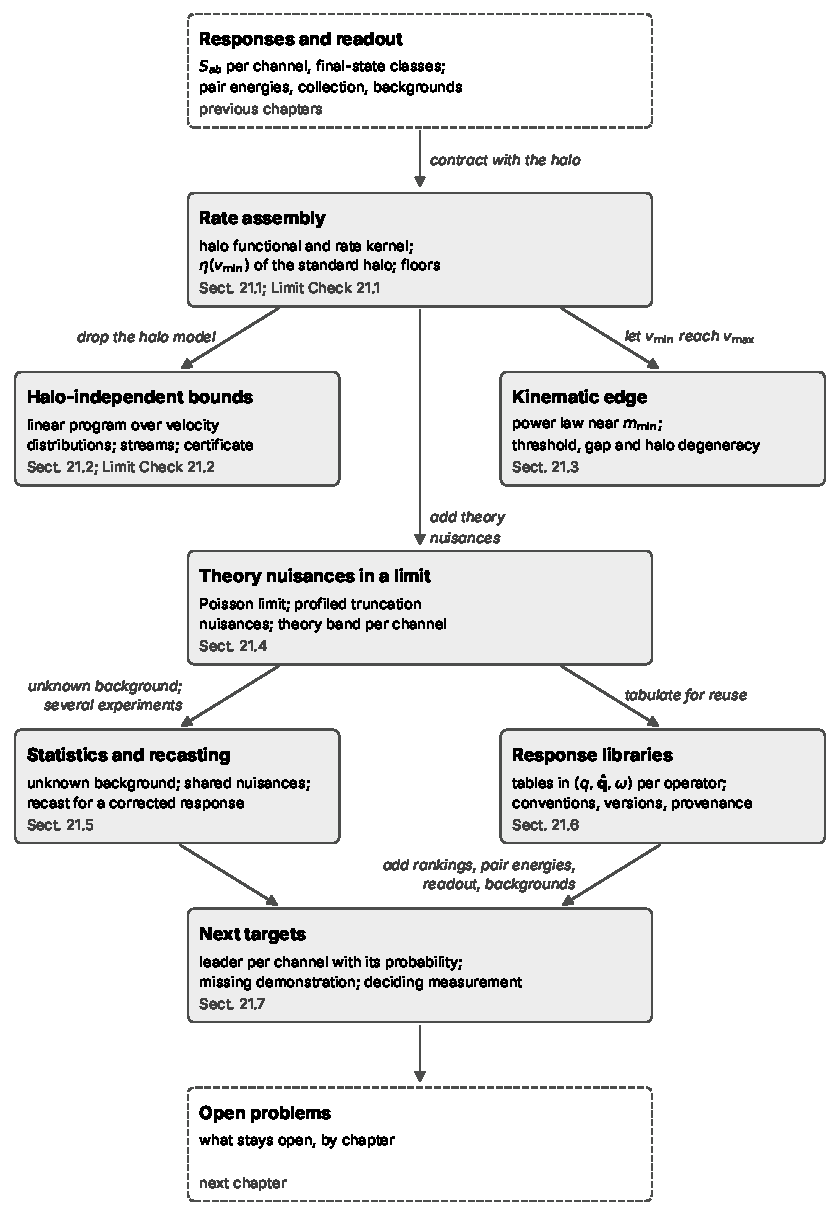
\includegraphics[width=0.78\linewidth]{figures/ch21/map21.pdf}
  \caption{From rates to limits and to the guide to next targets. The channel responses and the measured signal of the previous chapters are contracted with the halo into a rate per channel (\cref{sec:21.1}; \cref{lim:21.1a}). Three questions branch from it: what holds for every velocity distribution (\cref{sec:21.2}; \cref{lim:21.2a}), how the limit behaves where the minimum velocity reaches the largest speed in the halo (\cref{sec:21.3}), and how the theory uncertainties of each channel become a band on the limit (\cref{sec:21.4}). The band carries over to unknown backgrounds, combinations and recasts (\cref{sec:21.5}). The guide to next targets adds the rankings of the response, the pair energies, the readout and the backgrounds (\cref{sec:21.7}). The last box is the index of open problems of \cref{chap:22}.}
  \label{fig:21-map}
\end{figure}

\section{Rates as halo functionals}\label{sec:21.1}

The silicon rate of \cref{sec:10.2-corrections}, \num{5.9e4} events per kilogram and year at \SI{10}{MeV} for $\sigmae = \SI{e-37}{cm^2}$ with the random-phase loss function with local fields, rests on one velocity distribution, the standard halo of \cref{sec:1.2}. Simulated galaxies hold dark matter that this distribution does not describe. In the Via Lactea~II simulation, for instance, 22 percent of the dark matter near the Sun's radius is debris stripped from satellites that still survive, and it moves at a galactic speed near \SI{340}{km.s^{-1}}~\cite{kuhlen2012direct}. A limit compared with such a halo has to be recomputed, and the recomputation is cheap because every rate in this book is linear in $f_\chi$. We will write the rate of any channel as one integral of $f_\chi$ against a kernel that holds everything else: the coupling, the response, the kinematics and the readout.

\subsection{The halo functional of a channel}\label{sec:21.1-functional}

A detector counts events in bins of some observable, the number of pairs $N_{\mathrm{eh}}$ for a charge readout. The rate in one bin is \cref{eq:8.7-handoff}. In it the velocity integral is the outermost one, and everything inside it depends on $\vect{v}$ but not on the halo. We collect it into one function:
\begin{keyresult}[Halo functional of a channel]
\begin{equation}
  \mathcal{R}_{N_{\mathrm{eh}}}[f_\chi] = \frac{\rho_\chi}{\mchi\,\rho_T}\int\dd^3v\,f_\chi(\vect{v})\,\varGamma_{N_{\mathrm{eh}}}(\vect{v}) ,
  \label{eq:21.1-functional}
\end{equation}
with the \emph{rate kernel}, the inner integrals of \cref{eq:8.7-handoff} at fixed $\vect{v}$,
\begin{equation}
  \varGamma_{N_{\mathrm{eh}}}(\vect{v}) = \int\frac{\dd^3q}{(2\pi)^3}\sum_\Lambda\sum_{a,b}\mathfrak{D}_{ab}(\vect{q},\vect{v})\,S_{ab}(\vect{q},\omega_{\vect{q}};\Lambda)\,P_{\mathrm{casc}}(N_{\mathrm{eh}}|\Lambda) ,
  \label{eq:21.1-kernel}
\end{equation}
the rate at which one dark-matter particle of velocity $\vect{v}$ makes events with $N_{\mathrm{eh}}$ pairs.
\end{keyresult}
\noindent Summed over $N_{\mathrm{eh}}$, the kernel is the per-particle rate $\varGamma(\vect{v})$ of \cref{eq:8.2-rate}. For any other observable, a phonon energy or a bin of total deposited energy, $P_{\mathrm{casc}}$ is replaced by the probability that the event lands in that bin. The halo enters only through $f_\chi$ and $\rho_\chi$, the channel only through its kernel, and the rate is a linear functional of $f_\chi$: a halo made of two components gives the sum of their rates, weighted by their shares of the density.

The kernel is never negative, since $\mathfrak{D}$ and $S$ are positive semidefinite matrices (\cref{sec:8.2}) and $P_{\mathrm{casc}}$ is a probability. Adding dark matter at any velocity therefore never lowers a rate, which is the property on which the halo-independent bounds of \cref{sec:21.2} rest. The kernel vanishes at small speeds. A particle of speed $v$ reaches only the pairs $(q,\omega)$ with $\vmin(q,\omega) \le v$ (\cref{sec:1.3}), so $\varGamma(\vect{v}) = 0$ for $v$ below the onset speed $v_{\mathrm{on}}(\mchi)$, the smallest $\vmin$ over the support of the response. And for a crystal the kernel depends on the direction of $\vect{v}$ in crystal axes. The laboratory distribution is $f_{\mathrm{gal}}(\vect{v} + \vect{v}_{\mathrm{E}}(t))$ (\cref{eq:1.2-flab}), and the crystal turns with the Earth (\cref{eq:1.2-rotation}). Averaged over an exposure, \cref{eq:21.1-functional} becomes
\begin{equation}
  \bar{\mathcal{R}}_{N_{\mathrm{eh}}} = \frac{\rho_\chi}{\mchi\,\rho_T}\int\dd^3v_{\mathrm{gal}}\,f_{\mathrm{gal}}(\vect{v}_{\mathrm{gal}})\,\bigl\langle\varGamma_{N_{\mathrm{eh}}}\bigl(\vect{v}_{\mathrm{gal}} - \vect{v}_{\mathrm{E}}(t)\bigr)\bigr\rangle_t ,
  \label{eq:21.1-exposure}
\end{equation}
where $\langle\cdot\rangle_t$ averages over the live time, with the argument of $\varGamma$ rotated into crystal axes at each $t$. All time dependence is now in the kernel, and the exposure-averaged kernel at $\vect{v}_{\mathrm{gal}}$ is the rate that a single stream of dark matter at that velocity would produce.

Absorption fits the same form. The kernel is then $\varGamma_{\mathrm{abs}}$ of \cref{eq:8.2-abs}, which depends on $\vect{v}$ only through the momentum $\vect{p}_\phi = m_\phi\vect{v}$ and the energy $\omega_\phi \simeq m_\phi(1 + v^2/2)$. Where the response is smooth on the scale $m_\phi v \approx 10^{-3}m_\phi$, the kernel is constant across the halo and the rate depends on the halo through $\rho_\chi$ alone.

\subsection{The mean inverse speed}\label{sec:21.1-eta}

For a response averaged over the directions of $\vect{q}$, as in the crystal form factor of \cref{sec:10.1}, the kernel depends only on the speed. The angular average of the energy delta function is $\Theta(v - \vmin)/(2qv)$ (\cref{sec:1.3}), and for a coupling that does not depend on the dark-matter velocity
\begin{equation}
  \varGamma(v) = \frac{1}{v}\int_0^\infty\dd\omega\int\frac{q\,\dd q}{4\pi^2}\sum_{a,b}\mathfrak{D}_{ab}(q)\,\bar S_{ab}(q,\omega)\,\Theta\bigl(v - \vmin(q,\omega)\bigr) .
  \label{eq:21.1-gammav}
\end{equation}
With $F_\chi(v)$ the speed distribution of \cref{eq:1.2-Fspeed}, the rate is a one-dimensional integral, $\mathcal{R} = (\rho_\chi/\mchi\rho_T)\int_0^\infty\dd v\,F_\chi(v)\,\varGamma(v)$. The product $v\varGamma(v)$ is the response integrated over the part of the $(q,\omega)$ plane that a particle of speed $v$ can reach. It is zero below $v_{\mathrm{on}}$ and grows with $v$, because a faster particle reaches every pair that a slower one reaches and more.

The mean inverse speed appears when the order of the integrals is reversed. Since $\eta(u) = \int_u^\infty\dd v\,F_\chi(v)/v$ by \cref{eq:1.3-eta}, the speed distribution is $F_\chi(v) = -v\,\dd\eta/\dd v$. Integrating by parts,
\begin{equation}
  \mathcal{R} = \frac{\rho_\chi}{\mchi\,\rho_T}\int_0^\infty\dd u\;\eta(u)\,\frac{\dd}{\dd u}\bigl[u\varGamma(u)\bigr] ,
  \label{eq:21.1-etaform}
\end{equation}
with no boundary terms, because $u\varGamma(u)$ vanishes below $v_{\mathrm{on}}$ and $\eta$ vanishes above $v_{\mathrm{max}}$. The derivative of \cref{eq:21.1-gammav} replaces $\Theta(u - \vmin)$ by $\delta(u - \vmin)$: $\dd[u\varGamma]/\dd u$ is the response of the pairs whose minimum velocity is $u$, and it is never negative. Inserting it in \cref{eq:21.1-etaform} and doing the $u$ integral sets $u = \vmin(q,\omega)$ in $\eta$, which is the isotropic rate \cref{eq:A.8-rateiso} integrated over $\omega$.

A coupling that depends on the dark-matter velocity needs no halo function beyond $\eta$. The operators of \cref{tab:8-operators} depend on the velocity through $\vect{v}^\perp$, linearly except for $\mathcal{O}_2$, which is quadratic. So $\mathfrak{D}_{ab}$ is a polynomial in the transverse velocity $\vect{v}_{\mathrm{T}}$, the part of $\vect{v}$ perpendicular to $\vect{q}$; at zero mass splitting, $\Delta_\chi = 0$, the longitudinal part is fixed at $\vmin$ by the delta function, and $v_{\mathrm{T}}^2 = v^2 - \vmin^2$ (\cref{sec:8.1}). For an orientation-averaged response no direction is left in the plane perpendicular to $\vect{q}$. Odd powers of $\vect{v}_{\mathrm{T}}$ then average to zero, and even powers enter through $v_{\mathrm{T}}^2$ alone. The quadratic term has a second speed moment as its halo average:
\begin{equation}
  \int\dd^3v\,f_\chi(\vect{v})\,\frac{v^2 - u^2}{v}\,\Theta(v - u) = 2\int_u^\infty\dd u'\,u'\eta(u') = \eta_2(u) .
  \label{eq:21.1-eta2}
\end{equation}
To see this, differentiate the left side with respect to $u$. The boundary term at $v = u$ vanishes, because the integrand is zero there, and what is left is $-2u\,\eta(u)$; both sides vanish for $u \ge v_{\mathrm{max}}$. The same step applied to $(v^2 - u^2)^n$ gives $-2nu$ times the moment with $n - 1$, so the quartic term of $\mathcal{O}_2$ is fixed by $\eta_2$ and hence by $\eta$. The function $\eta_2$ of \cref{app:A.8} is therefore not an independent input. In the kernel form $\varGamma(v)$ contains the extra terms, and \cref{eq:21.1-functional} holds as written.

Now take the density row, $\mathfrak{D}_{ee} = \pi\sigmae\FDM^2/\mu_{\chi e}^2$ (\cref{eq:1.4-Vsq}), and the independent-particle structure factor $\bar S^0$ of \cref{sec:10.1}. \Cref{eq:21.1-etaform} is then \cref{eq:10.1-rateiso}, and written with the crystal form factor it is the rate with the crystal form factor \cref{eq:10.1-fcrys}, divided by the target mass~\cite[Eqs.~(3.13), (3.17)]{essig2016direct}. In the standard halo $\eta$ is the closed form of \cref{app:D.1}~\cite[App.~B]{essig2016direct}. With $S = (2q^2/e^2)L$ (\cref{eq:4.4-SL}) in place of $\bar S^0$, \cref{eq:21.1-etaform} is the loss-function rate \cref{eq:10.2-rate}, which the silicon kernels of this chapter use. One step separates that form from what \cref{app:A.8} prescribes for a rate averaged over an exposure. The closed form holds at one Earth speed, while over a year $|\vect{v}_{\mathrm{E}}(t)|$ runs from 237.4 to \SI{266.4}{km.s^{-1}} (\cref{sec:1.2}). The exposure average of $\eta$ is the average of the closed form over those speeds, and the question is when the closed form at $v_{\mathrm{E}}^{\mathrm{ref}} = \SI{250.5}{km.s^{-1}}$, the convention of \cref{app:A.8} and not the yearly mean of \SI{252.1}{km.s^{-1}}, can stand in for it. Write $|\vect{v}_{\mathrm{E}}(t)| = v_{\mathrm{E}}^{\mathrm{ref}} + \delta v_{\mathrm{E}}(t)$. Over a full year the term of \cref{eq:1.2-annual} that is linear in the orbital velocity averages to zero, and what is left is $\langle\delta v_{\mathrm{E}}\rangle = \SI{1.61}{km.s^{-1}}$, almost all of it from the second-order term, and $\langle\delta v_{\mathrm{E}}^2\rangle = \SI{108.3}{km^2.s^{-2}}$, an rms of \SI{10.4}{km.s^{-1}}. To second order,
\begin{equation}
  \langle\eta(u)\rangle_t - \eta(u)\big|_{v_{\mathrm{E}}^{\mathrm{ref}}} \simeq \frac{\partial\eta}{\partial v_{\mathrm{E}}}\,\langle\delta v_{\mathrm{E}}\rangle + \frac12\,\frac{\partial^2\eta}{\partial v_{\mathrm{E}}^2}\,\langle\delta v_{\mathrm{E}}^2\rangle .
  \label{eq:21.1-annualcorr}
\end{equation}
In the bulk of the halo both derivatives are small and the correction is a percent. Near the end point $\eta \propto \delta^2$ with $\delta = v_{\mathrm{esc}} + v_{\mathrm{E}} - u$ (\cref{eq:1.3-edge}), a convex function of $v_{\mathrm{E}}$, and the June excess outweighs the December deficit: the yearly average lies above the value at the mean speed.
\begin{limitbox}[Mean inverse speed of the standard halo][lim:21.1a]
For the truncated Maxwellian of \cref{eq:1.2-fgal} seen at Earth speed $v_{\mathrm{E}}$, and $\vmin < v_{\mathrm{esc}} - v_{\mathrm{E}}$,
\begin{equation*}
  \eta(\vmin) = \frac{\pi v_0^2}{v_{\mathrm{E}}N_{\mathrm{esc}}}\left\{\frac{\sqrt{\pi}\,v_0}{2}\left[\operatorname{erf}\frac{\vmin + v_{\mathrm{E}}}{v_0} - \operatorname{erf}\frac{\vmin - v_{\mathrm{E}}}{v_0}\right] - 2v_{\mathrm{E}}\,\ee^{-v_{\mathrm{esc}}^2/v_0^2}\right\} ,
\end{equation*}
with the second branch \cref{eq:D.1-eta2} up to $v_{\mathrm{esc}} + v_{\mathrm{E}}$~\cite[Eqs.~(B.4) and (B.5)]{essig2016direct}.
\par\smallskip
{\centering
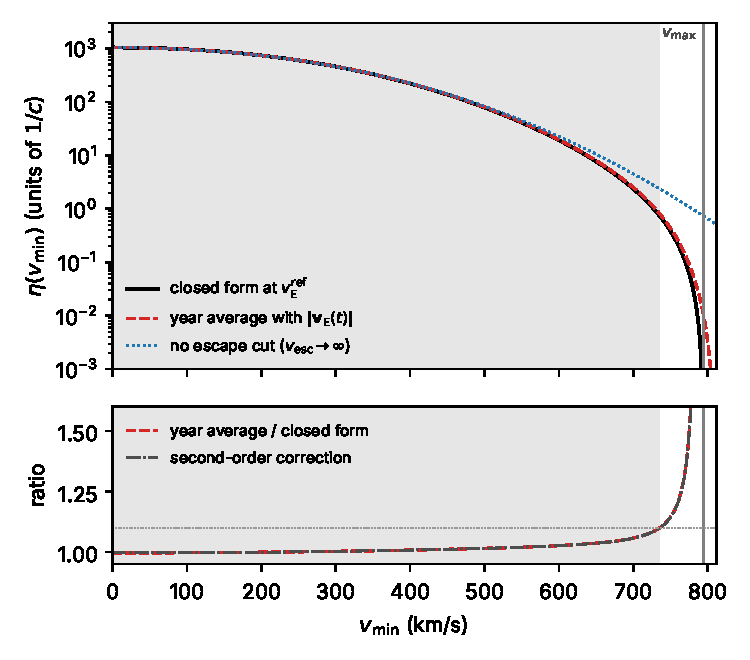
\includegraphics[width=\linewidth]{figures/ch21/limit21_1a.pdf}
\captionof{figure}{Mean inverse speed of the standard halo ($v_0 = \SI{238}{km.s^{-1}}$, $v_{\mathrm{esc}} = \SI{544}{km.s^{-1}}$) against $\vmin$. Top, in units of $1/c$: the closed form at the reference Earth speed $v_{\mathrm{E}}^{\mathrm{ref}} = \SI{250.5}{km.s^{-1}}$ (solid). Dashed: the fuller result, the same closed form averaged over a year with the exact Earth speed of \cref{eq:1.2-vE,eq:1.2-vorb} on 7305 equally spaced days. Dotted: the Maxwellian without the escape cut at $v_{\mathrm{E}}^{\mathrm{ref}}$. Bottom: the yearly average over the closed form (dashed) and the second-order correction \cref{eq:21.1-annualcorr} (dash-dotted). Gray: $\vmin \le \SI{735.6}{km.s^{-1}}$, where the yearly average exceeds the closed form at $v_{\mathrm{E}}^{\mathrm{ref}}$ by less than 10 percent (1 percent up to \SI{430.3}{km.s^{-1}}). The second-order correction stays within 1 percent of the yearly average up to \SI{786.3}{km.s^{-1}}. Vertical line: $v_{\mathrm{max}} = \SI{794.5}{km.s^{-1}}$.}\label{fig:21-limit-eta}
\par}
\smallskip
Within \SI{59}{km.s^{-1}} of $v_{\mathrm{max}}$ the yearly average exceeds the fixed-speed form by more than 10 percent, and above $v_{\mathrm{max}}$ it vanishes while the average stays positive up to \SI{810.4}{km.s^{-1}}.
\end{limitbox}
\noindent At $\vmin = 0$ the yearly average is 0.9965 of the closed form: the mean inverse speed itself barely moves. The ratio grows to 1.015 at \SI{500}{km.s^{-1}}, 1.026 at 600 and 1.057 at \SI{700}{km.s^{-1}}, then turns up steeply, to 1.20 at 760 and 1.78 at \SI{780}{km.s^{-1}}. The second-order term follows it within a few parts in a thousand to \SI{780}{km.s^{-1}}. The escape cut matters over a much wider range than the annual average does: without it, $\eta$ would be 1.18 times larger at \SI{600}{km.s^{-1}}, 1.90 times at 700 and 6.8 times at \SI{760}{km.s^{-1}}. Averaging $\eta$ over the year raises this silicon rate by 0.9 percent at \SI{10}{MeV} and by 5.6 percent at \SI{1}{MeV}, where the kernel opens near \SI{460}{km.s^{-1}}. Closer to the threshold mass the correction grows without bound, and \cref{sec:21.3} treats that regime.

\Cref{fig:21-kernel} shows the kernel of the silicon electron-recoil channel for a heavy mediator, built from the random-phase loss function with local fields of the tables of \cref{sec:10.2}, counted from their gap of \SI{1.17}{eV}. At \SI{10}{MeV} it opens at $v_{\mathrm{on}} = \SI{145}{km.s^{-1}}$, which is $(2\omega/\mchi)^{1/2}$ at the gap; the kernel, scaled to a rate per target mass as in \cref{fig:21-kernel}, is $\num{1.77e4}$ per kilogram and year at \SI{300}{km.s^{-1}}, $\num{1.28e5}$ at \SI{500}{km.s^{-1}} and $\num{3.11e5}$ at $v_{\mathrm{max}}$, for $\sigmae = \SI{e-37}{cm^2}$. Integrated against $F_\chi$ at $v_{\mathrm{E}}^{\mathrm{ref}}$, it returns \SI{5.897e4}{kg^{-1}.yr^{-1}}, the rate of \cref{sec:10.2-corrections}, and the form \cref{eq:21.1-etaform} returns the same number to five digits. At \SI{1}{MeV} the kernel opens only near \SI{460}{km.s^{-1}} and the rate, \SI{16.5}{kg^{-1}.yr^{-1}}, comes entirely from the fastest fifth of the halo. At \SI{100}{MeV} it opens at \SI{46}{km.s^{-1}} and changes by a factor of 4.0 between 300 and \SI{700}{km.s^{-1}}, against 14 at \SI{10}{MeV}. The heavier the particle, the flatter the kernel over the bulk of the halo, and the less the rate depends on the shape of $F_\chi$.
\begin{figure}[tbp]
  \centering
  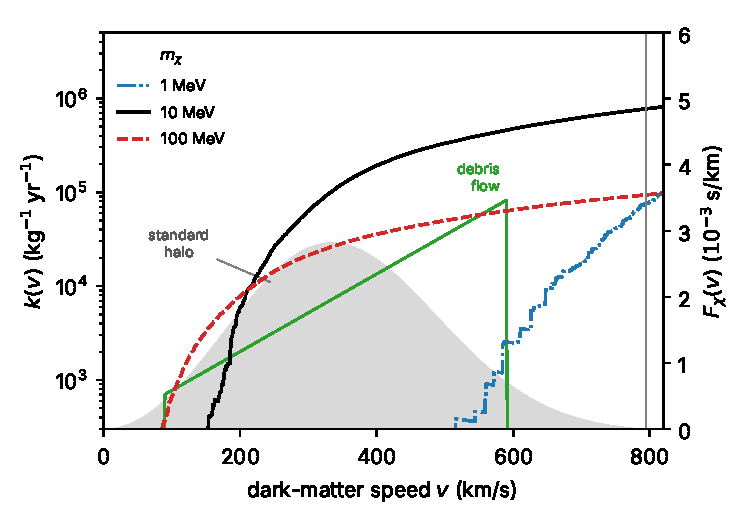
\includegraphics[width=0.8\linewidth]{figures/ch21/fig21_1.pdf}
  \caption{Rate kernel of the silicon electron-recoil channel, $\rho_\chi\varGamma(v)/\mchi\rho_T$ of \cref{eq:21.1-gammav}, the rate per unit target mass if all dark matter moved at speed $v$, for a heavy mediator, $\sigmae = \SI{e-37}{cm^2}$ and $\rho_\chi = \SI{0.3}{GeV.cm^{-3}}$, at $\mchi = 1$, 10 and \SI{100}{MeV} (left axis). The response is the direction-averaged random-phase loss function with local fields of Knapen, Kozaczuk and Lin~\cite{knapen2021dark} (\cref{sec:10.2}), from their gap of \SI{1.17}{eV}. Right axis: laboratory speed distributions at $v_{\mathrm{E}}^{\mathrm{ref}} = \SI{250.5}{km.s^{-1}}$ of the standard halo (gray, \cref{eq:1.2-Fspeed}) and of a debris flow of galactic speed \SI{340}{km.s^{-1}} (green, \cref{eq:21.1-fflow}). Vertical line: $v_{\mathrm{max}} = \SI{794.5}{km.s^{-1}}$.}
  \label{fig:21-kernel}
\end{figure}

\subsection{Threshold masses as floors}\label{sec:21.1-floor}

Where the kernel vanishes, so does the rate. By \cref{eq:21.1-functional}, a mass gives a nonzero rate only if the halo holds particles faster than $v_{\mathrm{on}}(\mchi)$. For a response whose onset $E_{\mathrm{th}}$ does not depend on $q$, the smallest $\vmin$ is $(2E_{\mathrm{th}}/\mchi)^{1/2}$ (\cref{sec:1.3}), and the condition $v_{\mathrm{on}} < v_{\mathrm{max}}$ is $\mchi > 2E_{\mathrm{th}}/v_{\mathrm{max}}^2$, the threshold mass of \cref{eq:1.3-mmin}. Quoted with $v_{\mathrm{max}} = v_{\mathrm{esc}} + v_{\mathrm{E}}^{\mathrm{ref}}$, that value is a floor, never the edge of a limit.

The onset of a real response depends on $q$. Then $v_{\mathrm{on}} = \min_q[E_{\mathrm{th}}(q)/q + q/2\mchi]$ lies above $(2E_{\mathrm{th}}/\mchi)^{1/2}$ with $E_{\mathrm{th}}$ the global minimum, and the edge lies above the floor. In silicon the floor at the gap, \SI{1.170}{eV}, is \SI{0.3332}{MeV}, and at the lowest excitation, the $1s$ exciton at \SI{1.1553}{eV}, it is \SI{0.3290}{MeV}; the edges of the pair channels lie above it (\cref{tab:9-edges}).

Near $v_{\mathrm{max}}$ the mean inverse speed $\eta$ vanishes quadratically (\cref{eq:1.3-edge}), and the reachable part of the response shrinks with it. A finite exposure therefore excludes only masses some distance above the floor, and how far above depends on the exposure, on the onset exponent of the response and on the tail of the halo. \Cref{sec:21.3} derives that distance.

The floor depends on the halo and on the Earth speed it is computed with. The reference speed fixes $v_{\mathrm{max}} = \SI{794.5}{km.s^{-1}}$ by convention (\cref{app:A.8}). In June the fastest particles move at $v_{\mathrm{esc}} + |\vect{v}_{\mathrm{E}}| = \SI{810.4}{km.s^{-1}}$, and an exposure that includes June has a nonzero rate down to a floor 3.9 percent lower, \SI{0.3202}{MeV} for the silicon gap; \cref{lim:21.1a} shows its origin in $\eta$. The annual motion is known kinematics, not an uncertainty: a limit uses the rate averaged over its exposure, June included (\cref{sec:21.3-degeneracy}), and the floor at the reference speed is the convention for comparing targets. Conversely, a halo component lowers the floor only if it carries particles faster than $v_{\mathrm{max}}$. A debris flow at \SI{340}{km.s^{-1}} reaches at most \SI{590.5}{km.s^{-1}} in the laboratory, and on its own it would give no silicon electron recoil below \SI{0.6031}{MeV}.

\subsection{A halo with a debris flow}\label{sec:21.1-debris}

Kuhlen, Lisanti and Spergel model the debris flow as an isotropic shell in velocity space: every particle has the same galactic speed $v_{\mathrm{flow}}$, in a random direction~\cite{kuhlen2012direct}. In the laboratory a particle of direction $\hat{\vect{v}}_{\mathrm{gal}}$ has speed $v$ with $v^2 = v_{\mathrm{flow}}^2 + v_{\mathrm{E}}^2 - 2v_{\mathrm{flow}}v_{\mathrm{E}}\cos\theta_{\mathrm{flow}}$, where $\theta_{\mathrm{flow}}$ is the angle between $\vect{v}_{\mathrm{gal}}$ and $\vect{v}_{\mathrm{E}}$. Since $\cos\theta_{\mathrm{flow}}$ is uniform on $[-1,1]$ and $v\,\dd v = -v_{\mathrm{flow}}v_{\mathrm{E}}\,\dd\cos\theta_{\mathrm{flow}}$, the laboratory speed distribution is~\cite[Eq.~(7)]{kuhlen2012direct}
\begin{equation}
  F_{\mathrm{flow}}(v) = \frac{v}{2v_{\mathrm{flow}}v_{\mathrm{E}}}\quad\text{for } |v - v_{\mathrm{flow}}| < v_{\mathrm{E}} ,
  \label{eq:21.1-fflow}
\end{equation}
and zero outside, for $v_{\mathrm{flow}} > v_{\mathrm{E}}$. Its mean inverse speed is $\eta_{\mathrm{flow}}(u) = 1/v_{\mathrm{flow}}$ for $u < v_{\mathrm{flow}} - v_{\mathrm{E}}$, falls linearly as $(v_{\mathrm{flow}} + v_{\mathrm{E}} - u)/(2v_{\mathrm{flow}}v_{\mathrm{E}})$ across the window, and vanishes above $v_{\mathrm{flow}} + v_{\mathrm{E}}$~\cite[Eq.~(8)]{kuhlen2012direct}. The halo is $f_\chi = (1 - p_{\mathrm{flow}})f_{\mathrm{SHM}} + p_{\mathrm{flow}}f_{\mathrm{flow}}$ at fixed total density, and in Via Lactea~II $p_{\mathrm{flow}} = 0.22$ and $v_{\mathrm{flow}} = \SI{340}{km.s^{-1}}$~\cite[Eq.~(10) and Fig.~6]{kuhlen2012direct}. Compared to the standard halo at the reference Earth speed, the flow has fewer slow particles, $\langle1/v\rangle = 1/v_{\mathrm{flow}}$, or 882 in natural units against 1041, and more fast ones: 55 percent of its particles move faster than \SI{400}{km.s^{-1}}, against 36 percent. It has none above \SI{590.5}{km.s^{-1}}.

\begin{workedexample}{The silicon rate in a halo with a debris flow}\label{we:21-debris}
Take silicon, $\mchi = \SI{10}{MeV}$, a heavy mediator and $\sigmae = \SI{e-37}{cm^2}$, with the kernel of \cref{fig:21-kernel} and $v_{\mathrm{E}} = v_{\mathrm{E}}^{\mathrm{ref}}$ for both components. The flow occupies $89.5 < v < \SI{590.5}{km.s^{-1}}$. Inserting \cref{eq:21.1-fflow} in \cref{eq:21.1-functional}, the factor $v$ of $F_{\mathrm{flow}}$ meets the factor $1/v$ of the kernel:
\begin{equation*}
  \mathcal{R}_{\mathrm{flow}} = \frac{1}{2v_{\mathrm{flow}}v_{\mathrm{E}}}\int_{v_{\mathrm{flow}} - v_{\mathrm{E}}}^{v_{\mathrm{flow}} + v_{\mathrm{E}}}\dd v\;v\,\frac{\rho_\chi\varGamma(v)}{\mchi\rho_T}
  = \frac{1}{v_{\mathrm{flow}}}\Bigl\langle v\,\frac{\rho_\chi\varGamma(v)}{\mchi\rho_T}\Bigr\rangle_{\mathrm{window}} .
\end{equation*}
Across the window the kernel rises from zero below \SI{145}{km.s^{-1}} through \SI{1.77e4}{kg^{-1}.yr^{-1}} at \SI{300}{km.s^{-1}}, \num{6.97e4} at 400 and \num{1.28e5} at \SI{500}{km.s^{-1}}, to \SI{1.82e5}{kg^{-1}.yr^{-1}} at \SI{590}{km.s^{-1}}. The mean of $v$ times the kernel over the window is \SI{2.769e7}{km.s^{-1}.kg^{-1}.yr^{-1}}, and
\begin{equation*}
  \mathcal{R}_{\mathrm{flow}} = \frac{\SI{2.769e7}{km.s^{-1}.kg^{-1}.yr^{-1}}}{\SI{340}{km.s^{-1}}} = \SI{8.145e4}{kg^{-1}.yr^{-1}} ,
\end{equation*}
the rate if all of the dark matter were in the flow. The form \cref{eq:21.1-etaform} with $\eta_{\mathrm{flow}}$ gives the same number. Per particle the flow is 1.381 times as effective as the standard halo, $\mathcal{R}_{\mathrm{SHM}} = \SI{5.897e4}{kg^{-1}.yr^{-1}}$, because it puts more particles where the kernel is large.

The mixed halo, by linearity, gives
\begin{equation*}
  \mathcal{R} = 0.78\times\num{5.897e4} + 0.22\times\num{8.145e4} = \SI{6.392e4}{kg^{-1}.yr^{-1}} ,
\end{equation*}
8.4 percent above the standard halo, or 175 events per kilogram and day. The spectrum hardly changes shape: its mean moves from 6.59 to \SI{6.62}{eV}. The flow's own spectrum ends at \SI{19.4}{eV}, the largest energy a particle at \SI{590.5}{km.s^{-1}} can deposit, against \SI{35}{eV} for the standard halo, and it peaks near \SI{6.0}{eV}, against \SI{5.4}{eV}.

The same halo changes the rate differently at other masses. For a light mediator at \SI{10}{MeV} the mixed rate is 8.8 percent above the standard one, and for a heavy mediator at \SI{100}{MeV}, 5.2 percent. At \SI{1}{MeV}, where the kernel opens near \SI{460}{km.s^{-1}}, the flow is only 0.28 times as effective as the standard halo, and the mixed rate falls 16 percent below it. A debris flow moves particles from both tails of the speed distribution into its middle. It raises the rate where the kernel opens in the bulk of the halo and lowers it near the threshold mass, which stays at the floor set by the standard component.
\end{workedexample}

\section{Halo-independent bounds}\label{sec:21.2}

A dark-matter particle of \SI{2}{MeV} can make an electron--hole pair in silicon only if it moves faster than \SI{325}{km.s^{-1}} in the laboratory, and a second pair only above \SI{466}{km.s^{-1}}, against the largest speed of the standard halo, $v_{\mathrm{max}} = \SI{794.5}{km.s^{-1}}$. A limit at that mass is therefore a statement about the fast part of the dark matter in the solar neighborhood, the part of the halo that \cref{sec:1.2} found least certain: changing the escape speed by \SI{25}{km.s^{-1}} changes $\eta$ at \SI{760}{km.s^{-1}} by a factor of 2.26 or 0.10. A statement that holds for every velocity distribution avoids the question. Because every count is a linear functional of $f_\chi$ (\cref{eq:21.1-functional}), the distributions that a null result allows form a convex set, and the largest value of any other linear quantity over that set is a semi-infinite linear program, with finitely many constraints on a measure over a continuum, the problem of \cref{app:C.12}. For silicon at 2 and \SI{10}{MeV}, dropping the halo model costs a factor of 2.0 to 3.7 in the bulk of the halo and orders of magnitude near $v_{\mathrm{max}}$.

\subsection{Stream kernels and the linear program}\label{sec:21.2-program}

The exposure-averaged rate \cref{eq:21.1-exposure} is an integral over galactic velocities $\vect{w}$ of the distribution $f_{\mathrm{gal}}$ times a kernel. Multiplied by the exposure $M_{\mathrm{det}}t_{\mathrm{exp}}$ it is a count. The local density, the cross-section and the mass multiply every rate in the combination $\rho_\chi\sigmae/\mchi$, which no count can separate from the normalization of $f_{\mathrm{gal}}$; the mass enters the kinematics as well, and the analysis is done at fixed $\mchi$. We therefore absorb the combination into a nonnegative measure $\Xi$ on the ball $\mathcal{B} = \{|\vect{w}| \le v_{\mathrm{esc}}\}$ and divide the kernel by $\sigmae$ (\cref{app:D.46}):
\begin{equation}
  \dd\Xi(\vect{w}) = \frac{\rho_\chi\sigmae}{\mchi}\,f_{\mathrm{gal}}(\vect{w})\,\dd^3w , \qquad
  \mathsf{k}_i(\vect{w}) = \frac{M_{\mathrm{det}}t_{\mathrm{exp}}}{\rho_T\,\sigmae}\,\bigl\langle\varGamma_i\bigl(\vect{w} - \vect{v}_{\mathrm{E}}(t)\bigr)\bigr\rangle_t ,
  \label{eq:21.2-stream}
\end{equation}
with $\varGamma_i$ the rate kernel \cref{eq:21.1-kernel} for bin $i$ of the observable. The expected count in bin $i$ is then $\int\mathsf{k}_i\,\dd\Xi$. The \emph{stream kernel} $\mathsf{k}_i(\vect{w})$ is the count that a single stream of unit $\Xi$-mass at $\vect{w}$ would leave in bin $i$; it contains the coupling up to its strength, the response, the final-state weights and the exposure, and nothing about the halo. A measured null result in bin $i$ becomes the constraint $\int\mathsf{k}_i\,\dd\Xi \le N_i^{\mathrm{up}}$, with $N_i^{\mathrm{up}}$ the upper count of \cref{sec:1.5} at the chosen confidence.

The quantity to bound is a second linear functional, $\int\mathsf{f}\,\dd\Xi$: the mean inverse speed above $u_0$ in the laboratory, the count of a second experiment, or a modulation amplitude. The mean inverse speed is the object of the standard halo-independent analysis,
\begin{equation}
  \tilde\eta(u_0) = \int\frac{\Theta(|\vect{w} - \vect{v}_{\mathrm{E}}| - u_0)}{|\vect{w} - \vect{v}_{\mathrm{E}}|}\,\dd\Xi(\vect{w}) = \frac{\rho_\chi\sigmae}{\mchi}\,\eta(u_0) ,
  \label{eq:21.2-etatilde}
\end{equation}
which is $\tilde\eta$ of \cref{app:A.8} with $\vect{v}_{\mathrm{E}}$ held fixed. Its value for the standard halo at a given $\sigmae$ is a curve in the plane of $u_0$ and $\tilde\eta$, and a bound on $\tilde\eta$ at every $u_0$ is the halo-independent counterpart of an exclusion curve. The count expected in a second experiment, $\mathsf{f} = \mathsf{k}^{\mathrm{B}}_j$, compares two targets, or one crystal at two orientations, without a halo model. A modulation amplitude, the difference of the kernels of two time bins, is a signed functional, bounded only if every stream on which it is positive is seen by some bin. The program is \cref{eq:C.12-sip} with these kernels.

By \cref{app:C.12}, any vector $\boldsymbol\lambda \ge 0$ with $\sum_i\lambda_i\mathsf{k}_i \ge \mathsf{f}$ on all of $\mathcal{B}$, a \emph{dual certificate}, proves $\int\mathsf{f}\,\dd\Xi \le \int\sum_i\lambda_i\mathsf{k}_i\,\dd\Xi \le \sum_i\lambda_iN_i^{\mathrm{up}}$ for every allowed halo at once, \cref{eq:C.12-certificate}. Checking it needs one function evaluated on the ball, not the optimizer that produced it. And the optimum is attained by a halo of at most $n$ streams for $n$ bins, $\Xi^* = \sum_a\xi_a\delta_{\vect{w}_a}$ with $\Xi$-masses $\xi_a$, placed at the zeros of the dual function $\mathsf{g}_\lambda = \sum_i\lambda_i\mathsf{k}_i - \mathsf{f}$. The extremal halos are therefore cold streams, far from any equilibrium model, and the bound holds for every halo because it holds for them. With the normalization of $f_\chi$ as an extra equality constraint the optimum allows one more stream~\cite[Eqs.~(14)--(19)]{ibarra2017optimized}, and any likelihood, not only a bound, is maximized by a sum of streams~\cite{gelmini2017unified}.

All bins of a search constrain one halo, so a bound derived from them is a statement about the event that every bin stays below its $N_i^{\mathrm{up}}$. If each bin is set at confidence $1 - \alpha_i$, that event has probability at least $1 - \sum_i\alpha_i$ by the union bound, and the bounds at all $u_0$ hold together at that level. The examples below use three pair bins with $N_i^{\mathrm{up}} = \ln 30 = 3.401$ each, the zero-event Poisson limit at 96.7 percent, so that the three bins hold jointly at 90 percent or more.

\subsection{The bound for a speed-only response}\label{sec:21.2-iso}

For a response averaged over the directions of $\vect{q}$, as in the crystal form factor of \cref{sec:10.1}, and with $\vect{v}_{\mathrm{E}}$ fixed, the stream kernel depends only on the laboratory speed $v = |\vect{w} - \vect{v}_{\mathrm{E}}|$. By \cref{eq:21.1-gammav} it is $\mathsf{k}_i(v) = \mathcal{A}_i(v)/v$, with the \emph{step column}
\begin{equation}
  \mathcal{A}_i(v) = \frac{M_{\mathrm{det}}t_{\mathrm{exp}}}{\rho_T\,\sigmae}\,v\,\varGamma_i(v) = \frac{M_{\mathrm{det}}t_{\mathrm{exp}}}{\rho_T\,\sigmae}\int\dd\omega\int\frac{q\,\dd q}{4\pi^2}\,\bar s_i(q,\omega)\,\Theta\bigl(v - \vmin(q,\omega)\bigr) ,
  \label{eq:21.2-column}
\end{equation}
where $\bar s_i$ is the angle-averaged response contracted with $\mathfrak{D}$ and weighted with the probability $P(i|\Lambda)$ of landing in bin $i$. The column is the count in bin $i$ for the step $\tilde\eta(u) = \Theta(v - u)$: all of $\tilde\eta$ sits below the speed $v$, the halo of a single stream at $v$. In silicon with the loss function of \cref{sec:10.2}, written as a crystal form factor by \cref{eq:A.8-fcrys,eq:4.4-SL}, the prefactor $M_{\mathrm{det}}t_{\mathrm{exp}}\,\alpha m_e^2/(M_{\mathrm{cell}}\mu_{\chi e}^2)$, with $M_{\mathrm{cell}}$ the mass of the two-atom unit cell, turns the column into a sum over the table, and $\mathcal{A}_i$ comes out in years for $\tilde\eta$ in inverse years. For a positive response the column never decreases with $v$ (\cref{eq:D.46-monotone}), since a faster particle reaches every pair that a slower one does (\cref{sec:21.1-eta}).

Monotonicity solves the program:
\begin{keyresult}[Halo-independent bound for a speed-only response]
For a response that depends only on $|\vect{q}|$, nonnegative bin weights, a fixed $\vect{v}_{\mathrm{E}}$, $0 < u_0 \le v_{\mathrm{max}}$ and $\max_i\mathcal{A}_i(u_0) > 0$, every velocity distribution allowed by the bins satisfies
\begin{equation}
  \tilde\eta(u_0) \le \min_i\frac{N_i^{\mathrm{up}}}{\mathcal{A}_i(u_0)} ,
  \label{eq:21.2-hib}
\end{equation}
and the bound is attained. The optimal halo is one stream at laboratory speed $u_0$ in any allowed direction, and the certificate is $\lambda_j = 1/\mathcal{A}_j(u_0)$ on the minimizing bin $j$, zero on the others.
\end{keyresult}
\noindent \Cref{app:D.46} gives the proof: the stream is feasible and reaches the bound, and the certificate holds because $\mathcal{A}_j(v) \ge \mathcal{A}_j(u_0)$ for $v \ge u_0$. With several bins the minimum over bins is the exact optimum, not an estimate, because one dual weight certifies it; the other bins are not saturated by the optimal stream and carry no weight. A column that decreases somewhere, which a truncated response with negative pieces can produce, leaves the single-bin value $N_i^{\mathrm{up}}/\inf_{v \ge u_0}\mathcal{A}_i(v)$ of \cref{eq:C.12-onebin} and voids the closed form for several bins (\cref{app:D.46}). And a bound on the galactic speed integral $\int\Theta(|\vect{w}| - u_0)|\vect{w}|^{-1}\dd\Xi$, in place of the laboratory speed $|\vect{w} - \vect{v}_{\mathrm{E}}|$ on which the kernel depends, is a different program, and \cref{eq:21.2-hib} does not answer it.

\Cref{fig:21-hib} applies \cref{eq:21.2-hib} to a silicon search of one kilogram-year that records no event in the one-, two- and three-pair bins, for a heavy mediator. A deposit $\omega$ lands in bin $i$ with the probability $P_{\mathrm{casc}}(i|\omega)$ of the cascade of \cref{sec:18.3}, the book's calibrated model with $\Eg = \SI{1.160}{eV}$ and \SI{3.749}{eV} per pair, computed for the seed of a dark-matter kick and applied at every $q$. The probability of the one-pair bin exceeds one half from 1.2 to \SI{6.2}{eV}, that of the two-pair bin from 6.3 to \SI{9.5}{eV} and that of the three-pair bin from 9.7 to \SI{13.1}{eV}, and a second pair is possible from about \SI{2.5}{eV}. Each bin gives a curve $N_i^{\mathrm{up}}/\mathcal{A}_i(u_0)$ that comes down from infinity at the onset speed of the bin, the smallest $\vmin$ among the pairs it can contain, and flattens as the column saturates; the bound is their lower envelope. At \SI{10}{MeV} the one-pair bin sets it below \SI{481.8}{km.s^{-1}}, the two-pair bin up to \SI{757.3}{km.s^{-1}} and the three-pair bin above. At \SI{2}{MeV} the one-pair bin sets it at every speed: the two-pair bin opens at \SI{465.9}{km.s^{-1}} and the three-pair bin at \SI{611.8}{km.s^{-1}}, and at $v_{\mathrm{max}}$ their columns are 2.4 and 206 times smaller. The dashed curves are $\tilde\eta$ of the standard halo at the cross-section where it first reaches $N_i^{\mathrm{up}}$ in some bin: $\sigmae = \SI{1.17e-41}{cm^2}$ at \SI{10}{MeV} and \SI{1.12e-40}{cm^2} at \SI{2}{MeV}, both set by the one-pair bin.

The standard curve lies below the bound at every $u_0$, as it must. The count of any halo in bin $j$ is $\int_0^\infty\tilde\eta(u)\,\dd\mathcal{A}_j(u)$, \cref{eq:21.1-etaform} in these variables, and since $\tilde\eta$ never increases and $\mathcal{A}_j$ never decreases, it is at least $\tilde\eta(u_0)\mathcal{A}_j(u_0)$. A halo that crossed the bound at some $u_0$ would overshoot $N_j^{\mathrm{up}}$. The ratio of the bound to the standard curve is the cost of dropping the halo model. It is smallest at \SI{381}{km.s^{-1}} for \SI{10}{MeV}, a factor 2.00, and near \SI{635}{km.s^{-1}} for \SI{2}{MeV}, a factor 3.70. Toward $v_{\mathrm{max}}$ it opens to 9.6 at \SI{600}{km.s^{-1}} and 63 at \SI{700}{km.s^{-1}} for \SI{10}{MeV}, because the standard halo has few particles there while a stream can put all its density at one speed. The curves hold for an exposure at the reference Earth speed; over a year the standard curve near $v_{\mathrm{max}}$ follows the year average of \cref{sec:21.1}, 1.06 times higher at \SI{700}{km.s^{-1}}.

\begin{figure}[tbp]
  \centering
  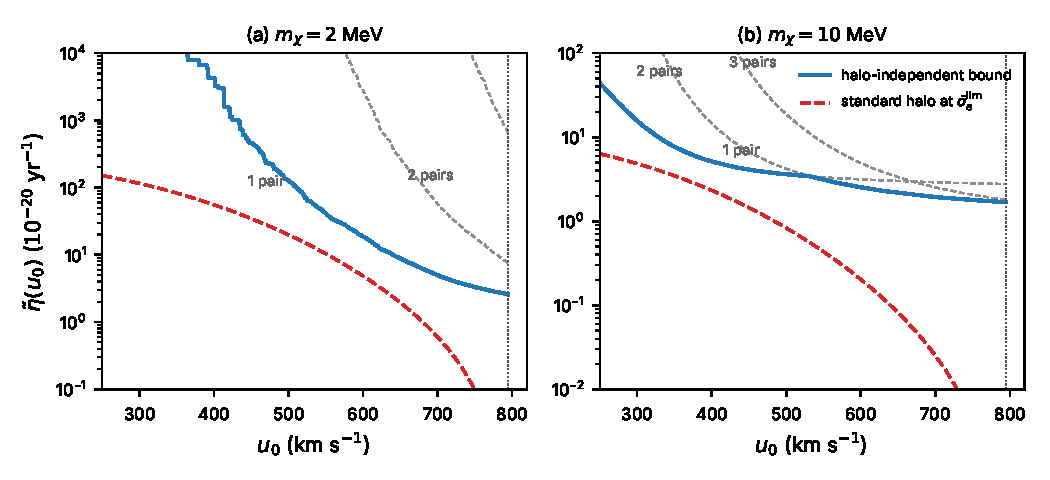
\includegraphics[width=\linewidth]{figures/ch21/fig21_2.pdf}
  \caption{Halo-independent bound on $\tilde\eta(u_0) = \rho_\chi\sigmae\eta(u_0)/\mchi$ for silicon, \cref{eq:21.2-hib} (solid), against $\tilde\eta$ of the standard halo at the cross-section of its own limit (dashed), for (a) $\mchi = \SI{2}{MeV}$ and (b) \SI{10}{MeV}, heavy mediator. Search: one kilogram-year at the reference Earth speed, no events in the one-, two- and three-pair bins, with the bin probabilities of the energy-only cascade of \cref{sec:18.3} (\SI{3.749}{eV} per pair), $N_i^{\mathrm{up}} = \ln 30$ in each bin, jointly at least 90 percent confidence. Gray dashed: single-bin bounds $N_i^{\mathrm{up}}/\mathcal{A}_i(u_0)$, labeled by the number of pairs; the solid curve is their lower envelope. Step columns from the direction-averaged random-phase loss function with local fields of Knapen, Kozaczuk and Lin (\cref{sec:10.2}), from \SI{1.17}{eV}. Standard halo: $v_0 = 238$, $v_{\mathrm{esc}} = \SI{544}{km.s^{-1}}$, $v_{\mathrm{E}}^{\mathrm{ref}} = \SI{250.5}{km.s^{-1}}$, at $\sigmae = \SI{1.12e-40}{cm^2}$ (a) and \SI{1.17e-41}{cm^2} (b). Dotted: $v_{\mathrm{max}} = \SI{794.5}{km.s^{-1}}$.}
  \label{fig:21-hib}
\end{figure}

\begin{workedexample}{One stream saturating a bound}\label{we:21-stream}
Take silicon at $\mchi = \SI{10}{MeV}$, a heavy mediator, the search of \cref{fig:21-hib} and $u_0 = \SI{500}{km.s^{-1}}$. The reduced mass is $\mu_{\chi e} = \SI{486.2}{keV}$, and the prefactor of the column, $M_{\mathrm{det}}t_{\mathrm{exp}}\,\alpha m_e^2/(M_{\mathrm{cell}}\mu_{\chi e}^2)$, is \SI{8.64e22}{yr} for one kilogram-year. Summing the cells of the table with $\vmin \le \SI{500}{km.s^{-1}}$, each weighted with its bin probability, gives
\begin{equation*}
  \mathcal{A}_1 = \SI{3.10e19}{yr} , \qquad \mathcal{A}_2 = \SI{3.48e19}{yr} , \qquad \mathcal{A}_3 = \SI{8.88e18}{yr} ,
\end{equation*}
for the one-, two- and three-pair bins. Divided into $N^{\mathrm{up}} = 3.401$ they give \num{1.10e-19}, \num{9.78e-20} and \SI{3.83e-19}{yr^{-1}}. The two-pair bin is tightest, and
\begin{equation*}
  \tilde\eta(\SI{500}{km.s^{-1}}) \le \frac{3.401}{\SI{3.48e19}{yr}} = \SI{9.78e-20}{yr^{-1}} .
\end{equation*}
The halo that reaches it is one stream at a laboratory speed of \SI{500}{km.s^{-1}}, $1.668\times10^{-3}$ in natural units, with $\Xi$-mass $\xi_1 = u_0N^{\mathrm{up}}/\mathcal{A}_2 = \SI{1.63e-22}{yr^{-1}}$. It leaves 3.03 events in the one-pair bin, 3.40 in the two-pair bin and 0.87 in the three-pair bin: only the two-pair bound is saturated. Its galactic speed lies between \num{249.5} and \SI{750.5}{km.s^{-1}} depending on its direction, and the directions against the Earth's motion are inside the escape speed.

The certificate is $\lambda_2 = 1/\mathcal{A}_2 = \SI{2.88e-20}{yr^{-1}}$ per event, $\lambda_1 = \lambda_3 = 0$, with value $\lambda_2N^{\mathrm{up}} = \SI{9.78e-20}{yr^{-1}}$, equal to the stream's. It is valid because $\mathcal{A}_2(v)/\mathcal{A}_2(u_0)$ never drops below 1 between \num{500} and \SI{794.5}{km.s^{-1}}, where it rises to 2.15.

The standard halo at its own limit, $\sigmae = \SI{1.17e-41}{cm^2}$, set by the one-pair bin, has $\tilde\eta(\SI{500}{km.s^{-1}}) = \SI{2.60e-20}{yr^{-1}}$, a factor 3.76 below the bound. The factor has two parts, read in the two-pair bin that sets the bound. The standard halo leaves only 2.47 events there, because the one-pair bin stops it first, and only 1.27 of them come from particles faster than \SI{500}{km.s^{-1}}; the bin allows $N^{\mathrm{up}} = 3.401$, a factor $3.401/1.266 = 2.69$ above what those particles use. And the fast particles move above \SI{500}{km.s^{-1}}, where the column is larger, so they produce 1.40 times the count of a stream at exactly \SI{500}{km.s^{-1}} with the same $\tilde\eta$. The stream avoids both losses, and $2.69 \times 1.40 = 3.76$.
\end{workedexample}

\subsection{Directional responses in the laboratory}\label{sec:21.2-dir}

A crystal resolves directions. Its response depends on $\hat{\vect{q}}$ in crystal axes, the crystal turns with the Earth, and a stream fixed in the galactic frame sweeps a cone of crystal directions every sidereal day (\cref{sec:11.7}). The stream kernel then depends on the direction of the stream, there is no step column, and the program has to be solved. Take a cubic crystal and a coupling that depends on $|\vect{q}|$ alone. The bin-weighted response is then $\bar s_i[1 + \sum_\ell a^i_\ell Y^{\mathrm{c}}_\ell(\hat{\vect{q}})]$, with the cubic harmonics of \cref{app:C.3}, $\ell = 4, 6, 8, \dots$ The energy delta function confines $\hat{\vect{q}}$ to a circle about the stream direction, at the angle $\arccos(\vmin/v)$, and the average of a harmonic over that circle is $P_\ell(\vmin/v)Y^{\mathrm{c}}_\ell(\hat{\vect{v}})$, \cref{eq:D.46-circle}. The kernel of a stream of velocity $\vect{v}$ in crystal axes is
\begin{equation}
  \mathsf{k}_i(\vect{v}) = \frac{M_{\mathrm{det}}t_{\mathrm{exp}}}{\rho_T\,\sigmae\,v}\int\dd\omega\int\frac{q\,\dd q}{4\pi^2}\,\bar s_i(q,\omega)\Bigl[1 + \sum_{\ell \ge 4}a^i_\ell(q,\omega)\,P_\ell\Bigl(\frac{\vmin}{v}\Bigr)Y^{\mathrm{c}}_\ell(\hat{\vect{v}})\Bigr]\Theta\bigl(v - \vmin(q,\omega)\bigr) ,
  \label{eq:21.2-multipole}
\end{equation}
before the average over the exposure (\cref{app:D.46}). Pairs with $\vmin$ close to $v$ are reached only by momentum transfers along the stream, $P_\ell \to 1$, and carry the full anisotropy of the response. Pairs with $\vmin \ll v$ are reached on a wide circle, and their anisotropy is reduced by $P_\ell(\vmin/v)$, which for $\ell \ge 4$ is at most 0.375 in magnitude as $\vmin/v \to 0$. The anisotropy of the kernel is therefore largest near the onset speed of each bin, where every reachable pair has $\vmin \approx v$.

The exposure average turns $Y^{\mathrm{c}}_\ell(\hat{\vect{v}})$ into its mean over the crystal directions that the stream visits. With $\vect{v}_{\mathrm{E}}$ fixed, a stream of laboratory speed $v$ and declination $\delta_{\mathrm{dec}}$ visits, over one sidereal day, the directions of \cref{eq:1.2-local} at all hour angles, and the mean depends on $\delta_{\mathrm{dec}}$, the latitude and the orientation of the crystal only. Streams with all right ascensions at a given $\delta_{\mathrm{dec}}$ therefore have the same kernel, and the program may place a stream at whichever right ascension the galactic support allows. That support, $|\vect{v} + \vect{v}_{\mathrm{E}}| \le v_{\mathrm{esc}}$, allows the declination $\delta_{\mathrm{dec}}$ at speed $v$ for some right ascension if $v^2 + |\vect{v}_{\mathrm{E}}|^2 - 2v|\vect{v}_{\mathrm{E}}|\cos(\delta_{\mathrm{dec}} + \delta_{\mathrm{E}}) \le v_{\mathrm{esc}}^2$, with $\delta_{\mathrm{E}} = 47.5^\circ$ the declination of $\vect{v}_\odot$ (\cref{sec:1.2}); the cosine is that of the smallest angle between $-\vect{v}$ and $\vect{v}_{\mathrm{E}}$ over right ascension. At $v_{\mathrm{max}}$ only $\delta_{\mathrm{dec}} = -\delta_{\mathrm{E}}$ remains, a stream that moves opposite to the Earth and arrives from the direction toward which the Sun moves. The program reduces to two variables, the speed and the declination of the stream.

\Cref{lim:21.2a} solves it for silicon at \SI{2}{MeV}, where every momentum transfer lies in the range of the model response of \cref{sec:11.7}. The isotropic part of the kernel comes from the loss function of \cref{fig:21-hib}. The ratios $a_\ell$ for $\ell = 4, 6, 8$ come from the cubic-harmonic components of the independent-particle structure factor of the empirical-pseudopotential model of \cref{sec:11.7}, applied at the same $(q,\omega)$. They are a model, with a gap of \SI{0.82}{eV} and no local fields, so the plot tests the method rather than measures silicon. The detector sits at \ang{45} north with $[001]$ vertical, $[100]$ east and $[010]$ north, the orientation of \cref{we:11-daily}, and records the search of \cref{fig:21-hib} in its one- and two-pair bins, integrated over sidereal time; the three-pair bin, open only above \SI{612}{km.s^{-1}} at this mass, never binds.

\begin{limitbox}[Speed-only bound against a directional response][lim:21.2a]
For a response averaged over the directions of $\vect{q}$ and a laboratory-frame stream~\cite[Eqs.~(A1)--(A2)]{fox2011integrating}: $\tilde\eta(u_0) \le \min_iN_i^{\mathrm{up}}/\mathcal{A}_i(u_0)$, \cref{eq:21.2-hib}. The formula ignores the anisotropy of the crystal; the plot shows how far the bound of the directional program departs from it.
\par\smallskip
{\centering
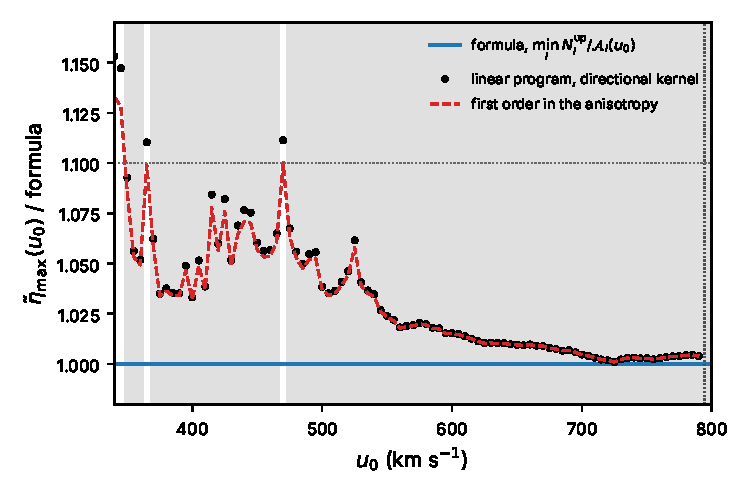
\includegraphics[width=\linewidth]{figures/ch21/limit21_2a.pdf}
\captionof{figure}{Largest $\tilde\eta(u_0)$ allowed by a silicon search over all halos, divided by the formula of the box (solid line at 1), against $u_0$. Dots: the fuller result, the linear program over galactic-frame streams with the direction-dependent kernel \cref{eq:21.2-multipole} of a crystal at \ang{45} north ($[001]$ up, $[100]$ east), integrated over the sidereal day, sampled from \SI{340}{km.s^{-1}} in steps of \SI{5}{km.s^{-1}}. Grid: \SI{2.5}{km.s^{-1}} in speed and \ang{2} in declination, with $|\vect{v}_{\mathrm{E}}| = \SI{250.5}{km.s^{-1}}$ toward declination \ang{47.5} and $v_{\mathrm{esc}} = \SI{544}{km.s^{-1}}$. Dashed: first order in the anisotropy, the formula divided by the smallest daily kernel of the tightest bin among the declinations allowed at $u_0$. $\mchi = \SI{2}{MeV}$, heavy mediator, one kilogram-year with no events in the one- and two-pair bins of the cascade of \cref{sec:18.3}, $N_i^{\mathrm{up}} = \ln 30$. Isotropic response: the random-phase loss function with local fields of Knapen, Kozaczuk and Lin; anisotropy: the $\ell = 4, 6, 8$ ratios of the empirical-pseudopotential model of \cref{sec:11.7} (a model). Gray: the formula lies within 10 percent of the linear program. Dotted: the 10 percent line and $v_{\mathrm{max}}$.}\label{fig:21-limit-hib}
\par}
\smallskip
Within \SI{20}{km.s^{-1}} of the one-pair onset, where every reachable pair sees the full anisotropy of the response, the formula falls short of the bound by up to 13 percent on the sampled speeds, and only the program gives a valid bound.
\end{limitbox}

The daily average removes most of the anisotropy. In the model the kernel of a stream fixed in crystal axes drops to 0.34 of its angle average in the least favorable direction. The sidereal mean of $Y^{\mathrm{c}}_4$, however, ranges only over $[-0.16, 0.07]$, against $[-0.43, 0.64]$ for $Y^{\mathrm{c}}_4$ itself. Over the declinations allowed at a given speed the daily kernel of the one-pair bin varies by $-7.3$ to $+3.1$ percent at \SI{500}{km.s^{-1}} and by $-2.3$ to $+1.7$ percent at \SI{600}{km.s^{-1}}. At every $u_0$ the program puts one stream at speed $u_0$, at the allowed declination where the daily kernel of the tightest bin is smallest, $-84^\circ$ at \SI{600}{km.s^{-1}}. The bound then exceeds the formula by the corresponding fraction: 2.3 percent at \SI{600}{km.s^{-1}}, 1.0 percent at \SI{700}{km.s^{-1}}, and no more than 4.6 percent anywhere above \SI{560}{km.s^{-1}}. The first-order estimate reproduces the program to 0.2 percent there and to 1.4 percent everywhere, because the optimum stays a single stream on a single bin. Below \SI{560}{km.s^{-1}} the ratio lies between 1.05 and 1.09 down to \SI{400}{km.s^{-1}}, because the pairs that enter the column near $u_0$ have $\vmin \approx u_0$ and see the full anisotropy, and at \SI{340}{km.s^{-1}}, \SI{15}{km.s^{-1}} above the one-pair onset at \SI{325}{km.s^{-1}}, it reaches 1.13. At \SI{790}{km.s^{-1}} the support leaves only declinations between $-56^\circ$ and $-40^\circ$, and the program lies 0.2 percent above the formula. A search binned in sidereal time keeps a kernel per time bin, close to the crystal-frame kernel for short bins, and its bound has to come from the program. The program then needs a response resolved in the direction of $\vect{q}$.

\subsection{Grids, certificates and leakage}\label{sec:21.2-leak}

A program solved on a grid of streams bounds the true optimum from below, since the grid can only restrict the halo, and its dual is a certificate only at the grid points. Between them the dual function can dip below zero. If the dip is at most $\delta_{\mathrm{cert}}$ on the support of $\mathsf{f}$, the dual still bounds every halo, at a price (\cref{app:D.46}):
\begin{equation}
  \int\mathsf{f}\,\dd\Xi \le \sum_i\lambda_iN_i^{\mathrm{up}} + \frac{\delta_{\mathrm{cert}}\,N_{\mathrm{tot}}}{\kappa_{\mathrm{v}}} ,
  \label{eq:21.2-defect}
\end{equation}
with $N_{\mathrm{tot}} = \sum_iN_i^{\mathrm{up}}$ and $\kappa_{\mathrm{v}}$ the smallest, over the support of $\mathsf{f}$, of the largest bin kernel, the visibility of \cref{eq:C.12-mass}. The second term is the violation times the largest halo mass the bins still allow on the support of $\mathsf{f}$. With $\delta_{\mathrm{cert}} = L_hh$, the Lipschitz constant of the dual function (the largest rate at which it changes per unit velocity) times the covering radius of the grid (the largest distance from a point of the support to the nearest grid point), it is the discretization bracket \cref{eq:C.12-leak}.

For the program of \cref{lim:21.2a} at $u_0 = \SI{600}{km.s^{-1}}$ a coarse and a fine grid agree in $\tilde\eta_{\max}$ to six digits, while the Lipschitz bracket is about 50 percent wide. The response is used on cells of \SI{0.01}{eV} by \SI{50}{eV} in momentum, and the kernel jumps whenever a cell's $\vmin$ crosses the speed of the stream, so a finite-difference Lipschitz constant measures the table, not the physics. The same structure gives an exact test. The isotropic part of a tabulated kernel is $\mathcal{A}_i(v)/v$ with $\mathcal{A}_i$ a step function, so the dual function changes its form only at the finitely many cell speeds $\vmin$; between them it is smooth. Evaluating the dual at those break speeds, with a Lipschitz bound only for the smooth anisotropic part $P_\ell(\vmin/v)$ between them, certifies it on the continuum.

A truncated response can also make a kernel negative, and then the mass bound behind \cref{eq:21.2-defect} fails for the computed kernel itself. Silicon gives the standard case. Outside the off-shell window, the Dyson convention of \cref{sec:8.6} splits the electronic response into a zero-phonon part and a phonon-dressed part whose sum is positive and whose parts need not be (\cref{eq:8.6-dyson}). The zero-phonon pair enters the cascade with the energy $\omega$, the phonon-dressed pair with $\omega - \omega_{\mathrm{ph}}$, and where the bin probability changes with energy the two are assigned to different bins. The bin-weighted response is then negative wherever one part is, but only where the bin probability changes within $\omega_{\mathrm{ph}}$. Seeding the phonon-dressed pair with the bin probability of its zero-phonon partner gives a kernel that is never negative, and \cref{eq:21.2-defect} applies to it with the difference of the two kernels added to $\delta_{\mathrm{cert}}$, weighted by $\lambda_i$. Suppose the number of pairs is stochastically ordered in the seed energy, so that the probability of at least $n$ pairs does not decrease with the energy for any $n$, as in the cascade of \cref{sec:18.3}. Then the total variation of each bin probability is at most 2, and the integral over energy of its change under a shift $\omega_{\mathrm{ph}} \le \omega_{\mathrm{max}}$ is at most $2\omega_{\mathrm{max}}$, one strip at each side of the bin (\cref{eq:D.46-tv}). Relative to the signal of a bin of width $\Delta_i$, the integral of its probability over energy,
\begin{equation}
  \frac{\text{misassigned weight in bin }i}{\text{signal in bin }i} \le \frac{2\,\omega_{\mathrm{max}}}{\Delta_i}\,\varrho^{\mathrm{leak}}_i ,
  \label{eq:21.2-fsleak}
\end{equation}
with $\varrho^{\mathrm{leak}}_i$ the largest phonon-dressed response over the bin, widened by $\omega_{\mathrm{max}}$ at each side, divided by the average of the total weighted with the bin probability, a number read off the computed response. For silicon, with the highest phonon at $\omega_{\mathrm{max}} = \SI{63.7}{meV}$ (\cref{sec:11.3}) and the two- and three-pair bins of the cascade of \cref{sec:18.3}, whose widths $\Delta_i$ are 3.60 and \SI{3.69}{eV}, close to $\varepsilon_{\mathrm{eh}} = \SI{3.749}{eV}$, the factor $2\omega_{\mathrm{max}}/\Delta_i$ is at most 0.035; the wider one-pair bin, \SI{4.98}{eV}, gives 0.026. The leakage is a few percent of $\varrho^{\mathrm{leak}}_i$ per bin. In the likelihood of \cref{sec:21.4} it is a normalization uncertainty of the bin with that width, and it enters the band of the limit.

\section{The kinematic edge}\label{sec:21.3}

A silicon detector that counts single electrons has no electron-recoil rate below the phonon-assisted onset, \SI{0.3374}{MeV} for free pairs (\cref{sec:13.1}), and just above it the rate grows as the $13/2$ power of the distance in mass (\cref{eq:13.9-medge}). In the model of \cref{fig:21-edge} the limit on $\sigmae$ is $1.6\times10^7$ times weaker \SI{0.001}{MeV} above the onset than at \SI{0.35}{MeV}, and still 4.6 times weaker \SI{0.010}{MeV} above it. Every mass up to \SI{0.010}{MeV} above the onset is tested only by particles within \SI{12}{km.s^{-1}} of $v_{\mathrm{max}}$, a fraction $6.0\times10^{-5}$ of the standard halo. The steep power, the position of the edge and its height therefore carry the halo model as much as the target. We will derive the power for any channel and any truncation of the halo, and work out which combinations of gap, threshold and halo parameters a limit near its edge measures.

\subsection{The rate kernel near its onset}\label{sec:21.3-kernel}

For a response averaged over the directions of $\vect{q}$, the rate is the speed integral $\mathcal{R} = (\rho_\chi/\mchi\rho_T)\int\dd v\, F_\chi(v)\,\varGamma(v)$ of \cref{sec:21.1-eta}. The kernel $\varGamma(v)$ of \cref{eq:21.1-gammav} vanishes below the onset speed $v_{\mathrm{on}}(\mchi)$ (\cref{sec:21.1-functional}), and the edge is decided by how it starts there. A particle of mass $\mchi$ and speed $v$ reaches the pair $(q,\omega)$ when $\vmin(q,\omega) \le v$, that is when $\omega \le qv - q^2/2\mchi$ (\cref{eq:1.3-vmin}). Let $E_{\mathrm{th}}(q)$ be the onset of the direction-averaged response at fixed $q = |\vect{q}|$, as in \cref{sec:13.9-onset}. We generalize the definition of \cref{sec:13.3} from the phonon-assisted loss function to any channel: the response rises above the onset as $x^{p_{\mathrm{on}}}$, with $x = \omega - E_{\mathrm{th}}(q)$. At fixed $q$ the energy integral then runs from $x = 0$ to the largest energy above the onset that the stream reaches,
\begin{equation*}
  x_{\mathrm{max}}(q; v) = qv - \frac{q^2}{2\mchi} - E_{\mathrm{th}}(q) ,
\end{equation*}
which is the $x_{\mathrm{max}}$ of \cref{sec:13.9-onset} with $v_{\mathrm{max}}$ replaced by $v$. The integral contributes $x_{\mathrm{max}}^{p_{\mathrm{on}}+1}/(p_{\mathrm{on}}+1)$ times the smooth factors of the channel: $F_{\mathrm{DM}}^2$, the powers of $q$ and the strength of the response.

The onset speed $v_{\mathrm{on}}(\mchi)$ is the speed at which the largest $x_{\mathrm{max}}$ reaches zero. Setting $v = v_{\mathrm{max}}$ and solving for the mass instead defines the edge mass of the channel,
\begin{equation}
  m_{\mathrm{edge}} = \min_q \frac{q^2}{2\,[qv_{\mathrm{max}} - E_{\mathrm{th}}(q)]} ,
  \label{eq:21.3-medge}
\end{equation}
which is \cref{eq:13.1-mPAdef} and \cref{eq:13.1-mZP} written for any onset. It reduces to $m_{\mathrm{min}}$ of \cref{eq:1.3-mmin} when $E_{\mathrm{th}}$ does not depend on $q$. Let $q^*$ be the optimal momentum transfer. Since $\partial x_{\mathrm{max}}/\partial v = q$, a stream slightly faster than $v_{\mathrm{on}}$ reaches $x_{\mathrm{max}}(q^*) = q^*(v - v_{\mathrm{on}})$ at the optimum, and near it
\begin{equation*}
  x_{\mathrm{max}}(q; v) \simeq q^*(v - v_{\mathrm{on}}) - \frac{(q - q^*)^2}{2\mchi} ,
\end{equation*}
where, as in \cref{sec:13.9-onset}, the curvature of $E_{\mathrm{th}}(q)$ is dropped against $1/\mchi$. That holds at the phonon-assisted onset; at the zero-phonon edge, where the onset rises steeply in $q$, the curvature changes the prefactor $\varGamma_{\mathrm{on}}$ below but not the exponent, which needs only a positive total curvature. The range of $q$ with $x_{\mathrm{max}} > 0$ has a width proportional to $(v - v_{\mathrm{on}})^{1/2}$, and the integral of $x_{\mathrm{max}}^{p_{\mathrm{on}}+1}$ over it is $(2\mchi)^{1/2}[q^*(v - v_{\mathrm{on}})]^{p_{\mathrm{on}}+3/2}B(\tfrac12, p_{\mathrm{on}}+2)$, with $B$ the Euler beta function. The kernel therefore starts as
\begin{equation}
  \varGamma(v) \simeq \varGamma_{\mathrm{on}}\,(v - v_{\mathrm{on}})^{p_{\mathrm{on}} + 3/2} , \qquad v \to v_{\mathrm{on}}^+ ,
  \label{eq:21.3-kernel}
\end{equation}
with a coefficient $\varGamma_{\mathrm{on}}$ that collects the strength of the response at the onset, $F_{\mathrm{DM}}^2(q^*)$ and the powers of $q^*$ and $\mchi$. The power $p_{\mathrm{on}} + 3/2$ counts $p_{\mathrm{on}} + 1$ from the energy integral and $\tfrac12$ from the width in $q$.

The $\tfrac12$ becomes 1 when $x_{\mathrm{max}}(q)$ has a corner at its maximum. If $x_{\mathrm{max}} \simeq x_{\mathrm{max}}(q^*) - s_\pm|q - q^*|$ with slopes $s_\pm$ on the two sides, the width in $q$ is linear in $v - v_{\mathrm{on}}$ and the power is $p_{\mathrm{on}} + 2$. A corner arises when the onset itself has a kink at $q^*$, or when the range of $q$ ends there. The second is the case of the free nuclear recoil with a detector threshold. Its response is the line $\omega = q^2/2M$, a delta function at fixed $q$, so the energy integral is a constant, which is the case $p_{\mathrm{on}} = -1$. The threshold cuts the range of momentum transfers at $q_{\mathrm{th}} = (2ME_{\mathrm{th}})^{1/2}$, and near the edge the optimum sits at that cut. The kernel of the free nuclear recoil therefore starts linearly, with power $-1 + 2 = 1$.

\subsection{The escape tail of the halo}\label{sec:21.3-tail}

The other factor of the speed integral, $F_\chi(v)$, vanishes at $v_{\mathrm{max}}$, and how it vanishes depends on how the galactic distribution goes to zero at the escape speed. The standard halo of \cref{tab:1-shm} is cut by hand (\cref{eq:1.2-fgal}), so the distribution in the galactic frame stays finite up to $v_{\mathrm{esc}}$ and then drops to zero. Equilibrium distribution functions built for the density profiles of simulated halos go to zero smoothly instead. Lisanti and co-workers write such a family as~\cite[Eq.~(1)]{lisanti2011dark}
\begin{equation*}
  f_{\mathrm{gal}}(u) \propto \left[\exp\!\left(\frac{v_{\mathrm{esc}}^2 - u^2}{k_{\mathrm{tail}}\,v_0^2}\right) - 1\right]^{k_{\mathrm{tail}}}\Theta(v_{\mathrm{esc}} - u) ,
\end{equation*}
which near the escape speed behaves as $(v_{\mathrm{esc}} - u)^{k_{\mathrm{tail}}}$~\cite[Eq.~(11)]{lisanti2011dark}. The \emph{tail exponent} $k_{\mathrm{tail}}$ is zero for the sharp cut of the standard halo and one for the King model, $f_{\mathrm{gal}} \propto \ee^{-u^2/v_0^2} - \ee^{-v_{\mathrm{esc}}^2/v_0^2}$~\cite[Eq.~(12)]{lisanti2011dark}. Their fits to the velocity distributions of simulated galactic halos prefer $k_{\mathrm{tail}}$ between 1.5 and 3.5~\cite[Sect.~II, Eq.~(10), and Fig.~3]{lisanti2011dark}. Near the escape speed, then, $f_{\mathrm{gal}} \simeq f_{\mathrm{esc}}\,y^{k_{\mathrm{tail}}}$ with $y = v_{\mathrm{esc}} - u$ and a constant $f_{\mathrm{esc}}$; for the standard halo $f_{\mathrm{esc}} = \ee^{-v_{\mathrm{esc}}^2/v_0^2}/N_{\mathrm{esc}}$, the height of the normalized distribution at the cut.

The laboratory speeds near $v_{\mathrm{max}} = v_{\mathrm{esc}} + v_{\mathrm{E}}$ come from a small cap of velocity space. The fastest particle has its galactic velocity antiparallel to $\vect{v}_{\mathrm{E}}$, so take the unit vector $\hat{\vect{e}} = -\vect{v}_{\mathrm{E}}/v_{\mathrm{E}}$ and write a laboratory velocity as $\vect{v} = (v_{\mathrm{max}} - s)\hat{\vect{e}} + \vect{v}_\perp$, with $s$ and $|\vect{v}_\perp|$ small. To second order in them the laboratory speed and the galactic speed are
\begin{equation*}
  v \simeq v_{\mathrm{max}} - s + \frac{v_\perp^2}{2v_{\mathrm{max}}} , \qquad
  u = |\vect{v} + \vect{v}_{\mathrm{E}}| \simeq v_{\mathrm{esc}} - s + \frac{v_\perp^2}{2v_{\mathrm{esc}}} .
\end{equation*}
A particle with $v \ge v_{\mathrm{max}} - \delta$ that is bound to the halo therefore has $0 \le y \le \delta - a_\perp v_\perp^2$, with $a_\perp = 1/2v_{\mathrm{esc}} - 1/2v_{\mathrm{max}} = v_{\mathrm{E}}/(2v_{\mathrm{esc}}v_{\mathrm{max}})$: a lens of depth $\delta$ and radius $(\delta/a_\perp)^{1/2}$. At fixed $\vect{v}_\perp$ the volume element is $\dd s = \dd y$, and the fraction of particles in the lens is
\begin{equation*}
  \int\!\dd^2v_\perp\int_0^{\delta - a_\perp v_\perp^2}\!\dd y\, f_{\mathrm{esc}}\,y^{k_{\mathrm{tail}}}
  = \frac{\pi f_{\mathrm{esc}}\,\delta^{k_{\mathrm{tail}}+2}}{a_\perp(k_{\mathrm{tail}}+1)(k_{\mathrm{tail}}+2)} .
\end{equation*}
Its derivative with respect to $\delta$ is the speed distribution at $v = v_{\mathrm{max}} - \delta$:
\begin{equation}
  F_\chi(v) \simeq F_{\mathrm{esc}}\,(v_{\mathrm{max}} - v)^{k_{\mathrm{tail}}+1} , \qquad
  F_{\mathrm{esc}} = \frac{2\pi f_{\mathrm{esc}}\,v_{\mathrm{esc}}v_{\mathrm{max}}}{(k_{\mathrm{tail}}+1)\,v_{\mathrm{E}}} ,
  \label{eq:21.3-tail}
\end{equation}
valid for $v_{\mathrm{max}} - v \ll v_{\mathrm{E}}, v_{\mathrm{esc}}$. Dividing by $v \simeq v_{\mathrm{max}}$ and integrating once more, $\eta(\vmin) \propto (v_{\mathrm{max}} - \vmin)^{k_{\mathrm{tail}}+2}$. For $k_{\mathrm{tail}} = 0$ this is the quadratic edge of \cref{eq:1.3-edge}, with its coefficient $A_\eta = \pi v_{\mathrm{esc}}\ee^{-v_{\mathrm{esc}}^2/v_0^2}/(v_{\mathrm{E}}N_{\mathrm{esc}}) = F_{\mathrm{esc}}/2v_{\mathrm{max}}$, so the lens reproduces the expansion of the closed form. For the smooth members the power law needs one more condition: the bracket of $f_{\mathrm{gal}}$ is linear in $y$ only for $y \ll k_{\mathrm{tail}}v_0^2/2v_{\mathrm{esc}}$, which is \SI{52}{km.s^{-1}} for the King model.

A smooth tail empties the lens. With the same $v_0$ and $v_{\mathrm{esc}}$, the $6.0\times10^{-5}$ of the standard halo within \SI{12}{km.s^{-1}} of $v_{\mathrm{max}}$, which decide every silicon mass up to \SI{0.010}{MeV} above the onset, become $4.7\times10^{-6}$ in the King model and $3.7\times10^{-8}$ for $k_{\mathrm{tail}} = 2.5$.

\subsection{The edge power law}\label{sec:21.3-power}

Both factors of the speed integral now start as powers, one at $v_{\mathrm{on}}$ and one at $v_{\mathrm{max}}$, and the integral is a beta function. Write $\delta_{\mathrm{on}} = v_{\mathrm{max}} - v_{\mathrm{on}}(\mchi)$ for the window of speeds that contribute. Inserting \cref{eq:21.3-kernel,eq:21.3-tail},
\begin{equation*}
  \begin{aligned}
  \mathcal{R} &\simeq \frac{\rho_\chi}{\mchi\rho_T}\,F_{\mathrm{esc}}\,\varGamma_{\mathrm{on}}\int_{v_{\mathrm{on}}}^{v_{\mathrm{max}}}\dd v\,(v_{\mathrm{max}} - v)^{k_{\mathrm{tail}}+1}(v - v_{\mathrm{on}})^{p_{\mathrm{on}}+3/2} \\
  &= \frac{\rho_\chi}{\mchi\rho_T}\,F_{\mathrm{esc}}\,\varGamma_{\mathrm{on}}\,B\bigl(k_{\mathrm{tail}}+2,\, p_{\mathrm{on}}+\tfrac52\bigr)\,\delta_{\mathrm{on}}^{\,p_{\mathrm{on}}+k_{\mathrm{tail}}+7/2} .
  \end{aligned}
\end{equation*}
The window is linear in the distance from the edge mass. The edge mass of \cref{eq:21.3-medge}, as a function of $v_{\mathrm{max}}$, changes by $\dd m_{\mathrm{edge}}/\dd v_{\mathrm{max}} = -q^{*3}/[2(q^*v_{\mathrm{max}} - E_{\mathrm{th}}(q^*))^2] = -2m_{\mathrm{edge}}^2/q^*$, since only the explicit dependence counts at the minimum. A mass $\mchi$ just above $m_{\mathrm{edge}}$ is therefore at its own edge for the speed $v_{\mathrm{on}} = v_{\mathrm{max}} - \delta_{\mathrm{on}}$ with
\begin{equation*}
  \delta_{\mathrm{on}} \simeq \frac{q^*}{2m_{\mathrm{edge}}^2}\,(\mchi - m_{\mathrm{edge}}) .
\end{equation*}
For a $q$-independent onset, $q^* = m_{\mathrm{min}}v_{\mathrm{max}}$ and this is the window $(v_{\mathrm{max}}/2)(\mchi - m_{\mathrm{min}})/m_{\mathrm{min}}$ of \cref{sec:1.3-edge}; at the phonon-assisted onset of silicon, \cref{eq:13.1-mPA} gives $q^* = m_{\mathrm{min}}^{\mathrm{PA}}(v_{\mathrm{max}} \pm u_\nu)$, with $u_\nu$ the group velocity of the phonon at $\vect{Q}^*$, equal to $m_{\mathrm{min}}^{\mathrm{PA}}v_{\mathrm{max}}$ up to $u_\nu/v_{\mathrm{max}} \sim 3\times10^{-3}$.

\begin{keyresult}[Edge power law]
Let the direction-averaged response of a channel rise as $x^{p_{\mathrm{on}}}$ above its onset, and let the galactic distribution of the halo vanish as $(v_{\mathrm{esc}} - u)^{k_{\mathrm{tail}}}$ at the escape speed. If the largest energy above the onset, $x_{\mathrm{max}}$, has a smooth maximum in $q$, the rate near the edge mass $m_{\mathrm{edge}}$ of \cref{eq:21.3-medge} is
\begin{equation}
  \mathcal{R}(\mchi) \propto (\mchi - m_{\mathrm{edge}})^{\,p_{\mathrm{on}} + k_{\mathrm{tail}} + 7/2} .
  \label{eq:21.3-power}
\end{equation}
If $x_{\mathrm{max}}$ has a corner, the power is $p_{\mathrm{on}} + k_{\mathrm{tail}} + 4$. The response contributes $p_{\mathrm{on}} + 1$, the width in $q$ one half (one at a corner), the halo $k_{\mathrm{tail}} + 1$, and the overlap of the two onsets one more. The power holds for either mediator, as long as $F_{\mathrm{DM}}$ is smooth at $q^* \neq 0$.
\end{keyresult}

For the standard halo, $k_{\mathrm{tail}} = 0$, \cref{eq:21.3-power} is \cref{eq:13.9-medge}. For the King model the silicon edge steepens from $13/2$ to $15/2$, and over the range preferred by simulated halos to between 8 and 10. The free nuclear recoil with a sharp threshold has a linear kernel and the power $3 + k_{\mathrm{tail}}$.

The power also sets how close to the edge an exposure reaches, the distance that \cref{sec:21.1-floor} left open. A background-free exposure excludes a mass at which it predicts more than 2.3 events (\cref{eq:1.5-N90}). Near the edge the predicted number is proportional to $M_{\mathrm{det}}t_{\mathrm{exp}}\sigmae(\mchi - m_{\mathrm{edge}})^{n}$, with the exposure $M_{\mathrm{det}}t_{\mathrm{exp}}$ and $n$ the power of \cref{eq:21.3-power}. At fixed $\sigmae$ the lowest excluded mass therefore lies at a distance from the edge proportional to $(M_{\mathrm{det}}t_{\mathrm{exp}}\sigmae)^{-1/n}$. At the free-pair edge of silicon, $n = 13/2$, ten times the exposure brings the excluded mass a factor $10^{-2/13} = 0.70$ closer to the edge; with the King tail the factor is 0.74.

\Cref{tab:21-edge} collects the powers of the silicon electron-recoil edges and the free nuclear recoil. The phonon-assisted entries use the onset exponents of \cref{sec:13.3,sec:13.8}. For the zero-phonon edge of \cref{sec:13.9-edges} the exponents follow from the counting rule of \cref{sec:13.3}: an isolated quadratic minimum in $D$ free variables gives $x^{D/2 - 1}$, and a vertex that vanishes linearly at the minimum adds one power. At fixed $|\vect{q}|$ a free zero-phonon pair has three free variables, the components of the hole's crystal momentum. The average over the two angles of $\hat{\vect{q}}$ adds two more, since each of the 24 equivalent optima of the first edge is an isolated minimum with curvatures $\beta_\theta$ and $\beta_z$ (\cref{sec:13.9-edges}). With $D = 5$ the pair would start as $x^{3/2}$. The first zero-phonon line, however, is second class: its vertex vanishes in the mirror plane and grows linearly with the distance from it (\cref{sec:13.9-glide}), so $p_{\mathrm{on}} = 5/2$. The Coulomb attraction lowers the onset exponent of a continuum at fixed $\vect{q}$ by one half, from $x^{1/2}$ to a step, as \cref{eq:13.8-edge} does for the phonon-assisted continuum, and the excitonic zero-phonon continuum has $p_{\mathrm{on}} = 2$. The $1s$ line is a delta function at fixed $\vect{q}$; the two angles turn it into a step and the vertex zero into $x^1$. Since the phonon-assisted rate is already open at \SI{0.405}{MeV}, these powers describe how the zero-phonon rate adds to the total, a kink in the rate rather than the edge of the limit.

\begin{table}[tbp]
  \caption{Powers of the rate in the dark-matter mass, $\mathcal{R} \propto (\mchi - m_{\mathrm{edge}})^{n}$, at the edges of silicon, for the sharp-cut standard halo ($k_{\mathrm{tail}} = 0$); a halo with tail exponent $k_{\mathrm{tail}}$ adds $k_{\mathrm{tail}}$ to every entry (\cref{eq:21.3-power}). Masses in MeV, with the halo of \cref{tab:1-shm}; $p_{\mathrm{on}}$ is the onset exponent of the direction-averaged response at fixed $|\vect{q}|$; the fourth column says whether $x_{\mathrm{max}}(q)$ has a smooth maximum or a corner at $q^*$ (\cref{eq:21.3-power}). The zero-phonon edges lie above the phonon-assisted onset, where they add a kink to the total rate. The nuclear-recoil row is for a \SI{10}{eV} threshold.}
  \label{tab:21-edge}
  \centering\small
  \begin{tabular}{@{}llccc@{}}
    \toprule
    Edge & $m_{\mathrm{edge}}$ & $p_{\mathrm{on}}$ & $x_{\mathrm{max}}$ at $q^*$ & $n$ \\
    \midrule
    Phonon-assisted, free pair (transverse acoustic) & 0.3374 & 3 & smooth & $13/2$ \\
    Phonon-assisted, excitonic continuum & 0.3374 & $5/2$ & smooth & 6 \\
    Phonon-assisted, exciton replica & 0.3332 & $3/2$ & smooth & 5 \\
    Zero-phonon, first edge, free pair & 0.405--0.408 & $5/2$ & smooth & 6 \\
    Zero-phonon, first edge, excitonic continuum & 0.405--0.408 & 2 & smooth & $11/2$ \\
    Zero-phonon, first edge, $1s$ line & 0.402--0.405 & 1 & smooth & $9/2$ \\
    Free nuclear recoil, sharp threshold & 137 & $-1$ & corner & 3 \\
    \bottomrule
  \end{tabular}
\end{table}

\Cref{fig:21-edge}(b) checks \cref{eq:21.3-power} in the model of \cref{sec:13.9-onset}: the computed transverse acoustic onset on the valley axis, a loss function $Cx^3$ and the family of halos above. The local power of the rate is $p_{\mathrm{on}} + k_{\mathrm{tail}} + 7/2$ to 0.002 up to \SI{3e-4}{MeV} above the onset for $k_{\mathrm{tail}} = 0$, 1 and 2.5. For the standard halo it drifts to 6.54 at \SI{0.005}{MeV} and 6.61 at \SI{0.02}{MeV}, as the curvature of the speed distribution enters; a light mediator leaves the power at 6.500 near the onset. The model loss function is the idealization. The computed one follows $x^3$ only for $x < \SI{1.3}{meV}$ (\cref{fig:13-paloss}), and since the largest energy above the onset grows as $x_{\mathrm{max}}^* = \tfrac12 v_{\mathrm{max}}^2(\mchi - m_{\mathrm{edge}})$, \SI{3.5}{meV} per \SI{0.001}{MeV}, the power is exact only within \SI{4e-4}{MeV} of the onset. At the zero-phonon edge, $x_{\mathrm{max}}^* = (q^{*2}/2m_{\mathrm{edge}}^2)(\mchi - m_{\mathrm{edge}})$ is \SI{5.3}{meV} per \SI{0.001}{MeV}; the $1s$ power holds while $x_{\mathrm{max}}^*$ stays below the exciton binding of \SI{14.7}{meV}, within \SI{0.0028}{MeV} of the line, and the continuum powers until neighboring optima merge \SI{49}{meV} above the edge (\cref{sec:13.9-rates}), \SI{0.009}{MeV} above it. The halo side is never the limitation at these masses: \SI{0.01}{MeV} above the onset the window is $\delta_{\mathrm{on}} = \SI{11.8}{km.s^{-1}}$, far inside the \SI{173}{km.s^{-1}} scale of the correction in \cref{eq:1.3-edge} and the \SI{52}{km.s^{-1}} range of the King tail.

\begin{figure}[tbp]
  \centering
  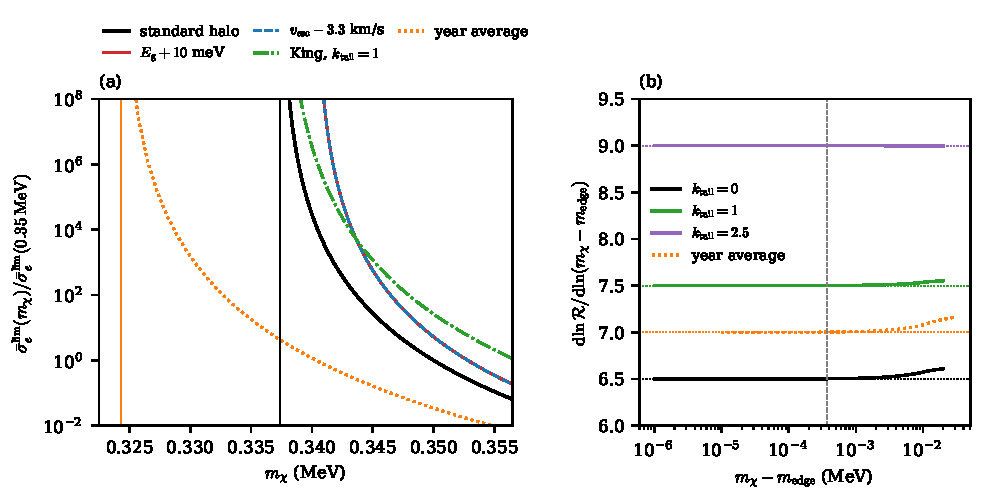
\includegraphics[width=\linewidth]{figures/ch21/fig21_3.pdf}
  \caption{The low-mass edge of a silicon electron-recoil limit. Model: direction-averaged loss function $Cx^3$ above the transverse acoustic onset on the valley axis ($m_{\mathrm{edge}} = \SI{0.33738}{MeV}$, PBE force constants of \cref{sec:5.2}, $\Eg = \SI{1.17}{eV}$), heavy mediator, background-free counting at fixed exposure, so that the limit is proportional to $1/\mathcal{R}$. (a)~Limit on $\sigmae$ relative to its value at \SI{0.35}{MeV}. Black: standard halo ($v_0 = 238$, $v_{\mathrm{esc}} = 544$, $v_{\mathrm{E}} = \SI{250.5}{km.s^{-1}}$). Red: gap raised by \SI{10}{meV}. Blue dashed, on top of the red curve: escape speed lowered by \SI{3.3}{km.s^{-1}} instead. Green dash-dotted: King model ($k_{\mathrm{tail}} = 1$) with the same $v_0$ and $v_{\mathrm{esc}}$. Orange dotted: an exposure spread uniformly over a year, with $v_{\mathrm{E}}$ between 237.4 and \SI{266.4}{km.s^{-1}}. Vertical lines: the edge at the reference speed and the June edge, \SI{0.3243}{MeV}. (b)~Local power of the rate, $\dd\ln\mathcal{R}/\dd\ln(\mchi - m_{\mathrm{edge}})$, for halos with tail exponents $k_{\mathrm{tail}} = 0$, 1 and 2.5 of the family of Lisanti and co-workers~\cite[Eq.~(1)]{lisanti2011dark} with the same $v_0$, $v_{\mathrm{esc}}$, $v_{\mathrm{E}}$, and for the year average ($m_{\mathrm{edge}}$ its June value). Dotted: the powers $p_{\mathrm{on}} + k_{\mathrm{tail}} + 7/2$ of \cref{eq:21.3-power} and $p_{\mathrm{on}} + 4$ for the year average. Dashed: the mass at which $x_{\mathrm{max}}^*$ reaches \SI{1.3}{meV}, the end of the $x^3$ range of the computed loss function.}
  \label{fig:21-edge}
\end{figure}

\subsection{Degeneracies at the edge}\label{sec:21.3-degeneracy}

Near its edge a limit is set by three numbers: the edge mass, the power and the height of the rate. Each is a combination of target and halo parameters, and parameters that enter the same combination cannot be told apart by the limit.

The edge mass depends on the onset $E_{\mathrm{th}}(q)$ and on $v_{\mathrm{max}} = v_{\mathrm{esc}} + v_{\mathrm{E}}$, and on nothing else. For a $q$-independent onset it depends on them only through $E_{\mathrm{th}}/v_{\mathrm{max}}^2$, the rule $\delta\ln m_{\mathrm{min}} = \delta\ln E_{\mathrm{th}} - 2\,\delta\ln v_{\mathrm{max}}$ of \cref{sec:1.3-edge}. The phonon-assisted onset of silicon depends on $q$, but \cref{eq:13.1-mPA} gives $m_{\mathrm{min}}^{\mathrm{PA}} = 2E_{\mathrm{on}}/(v_{\mathrm{max}}^2 - u_\nu^2)$ with the onset energy $E_{\mathrm{on}} = \Eg + \omega_\nu(\vect{Q}^*)$, and $u_\nu^2/v_{\mathrm{max}}^2 \sim 10^{-5}$. To that accuracy the edge measures the single ratio $E_{\mathrm{on}}/v_{\mathrm{max}}^2$. A one percent error in the onset energy $E_{\mathrm{on}}$, whether it comes from the gap, from the phonon energy that the onset adds or from the energy of a threshold of $n$ pairs, moves the edge exactly as a \SI{0.5}{\percent} change of $v_{\mathrm{max}}$, \SI{4.0}{km.s^{-1}}, does. Turned around, the escape-speed uncertainty of $\pm\SI{25}{km.s^{-1}}$ (\cref{sec:1.2}) moves the edge by $-6.0$ and $+6.6$ percent, as an error of $-71$ or $+78$~meV in the onset energy would, and the annual cycle of $v_{\mathrm{E}}$ by $-3.9$ and $+3.4$ percent.

The height of the rate is a product, $F_{\mathrm{esc}}\varGamma_{\mathrm{on}}$ in the speed integral above. The reference cross-section and the strength of the response at the onset sit in $\varGamma_{\mathrm{on}}$. The height $f_{\mathrm{esc}}$ of the galactic distribution at the cut and the geometric factor $v_{\mathrm{esc}}v_{\mathrm{max}}/v_{\mathrm{E}}$ of the lens sit in $F_{\mathrm{esc}}$. A null result near the edge bounds only the product. The dispersion $v_0$ enters the edge only here, through $f_{\mathrm{esc}}$: for the standard halo $\partial\ln A_\eta/\partial v_0 = 2v_{\mathrm{esc}}^2/v_0^3 - \partial\ln N_{\mathrm{esc}}/\partial v_0 = +\SI{3.2}{\percent}$ per km\,s$^{-1}$, so the uncertainty of $\pm\SI{6}{km.s^{-1}}$ (\cref{sec:1.2}) scales the rate near the edge by 1.21 and 0.83 at fixed edge mass. The escape speed enters both the edge mass and the height, but in the height its effect nearly cancels. At a fixed edge mass, lowering $v_{\mathrm{esc}}$ raises $A_\eta$ by \SI{1.76}{\percent} per km\,s$^{-1}$, since the cut moves into denser parts of the Maxwellian. It also lowers the powers of $v_{\mathrm{max}}$ in the rate. With the $q^3$ of \cref{eq:10.2-rate}, the energy integral of \cref{sec:13.9-onset} and $q^* = \mchi v_{\mathrm{max}}$, the rate at fixed $\mchi - m_{\mathrm{edge}}$ and fixed edge mass, with the gap moved together with $v_{\mathrm{esc}}$, scales as $A_\eta v_{\mathrm{max}}^{2p_{\mathrm{on}}+8}$ for a heavy mediator. For $p_{\mathrm{on}} = 3$ the factor $v_{\mathrm{max}}^{14}$ changes by \SI{1.76}{\percent} per km\,s$^{-1}$ as well, and the two changes cancel. A light mediator removes four powers of $v_{\mathrm{max}}$ through $F_{\mathrm{DM}}^2 \propto q^{*-4}$ and leaves \SI{0.5}{\percent} per km\,s$^{-1}$.

The power is a sum, $p_{\mathrm{on}} + k_{\mathrm{tail}}$, and the sum is all that a counting experiment can measure. The two exponents do enter the spectrum separately. At fixed $\omega$ the integral over $q$ of $\eta \propto (v_{\mathrm{max}} - \vmin)^{k_{\mathrm{tail}}+2}$, with $v_{\mathrm{max}} - \vmin = (x_{\mathrm{max}}(q) - x)/q$, runs over a range of width $\propto (x_{\mathrm{max}}^* - x)^{1/2}$ and gives
\begin{equation*}
  \frac{\dd\mathcal{R}}{\dd\omega} \propto (\omega - E_{\mathrm{on}})^{p_{\mathrm{on}}}\,(\omega_{\mathrm{top}} - \omega)^{k_{\mathrm{tail}} + 5/2} , \qquad \omega_{\mathrm{top}} = E_{\mathrm{on}} + x_{\mathrm{max}}^* ,
\end{equation*}
for an onset that is flat near $q^*$. The response shapes the bottom of the spectrum and the halo its top. The whole spectrum, however, is \SI{3.5}{meV} wide per \SI{0.001}{MeV} above the edge, while a silicon detector that counts pairs puts every deposit between $\Eg$ and $2\Eg$ into one bin (\cref{sec:1.5}). The bin integrates the spectrum, and with it the two exponents into their sum.

Two handles distinguish the target from the halo. The first is a second edge with a different mixture. At the zero-phonon edge the onset rises steeply with the distance of $\vect{q}$ from the valley, and the envelope theorem, by which only the explicit dependence of a minimized function on a parameter counts at its minimum (\cref{sec:21.3-power}), applied to \cref{eq:13.1-mZP} leads to $\partial\ln m_{\mathrm{min}}^{\mathrm{ZP}}/\partial\ln\Eg = \Eg/(q^*v_{\mathrm{max}} - E^*)$ and $\partial\ln m_{\mathrm{min}}^{\mathrm{ZP}}/\partial\ln v_{\mathrm{max}} = -q^*v_{\mathrm{max}}/(q^*v_{\mathrm{max}} - E^*)$, with $E^*$ the pair energy at the optimum and a rigid shift of the conduction bands. At the joint minimum of \cref{sec:13.9-edges}, $|\vect{q}^*| = \SI{1.33}{keV}$ and $E^* = \SI{1.355}{eV}$, these are 0.54 and $-1.62$, against 1 and $-2$ at the phonon-assisted onset. Two edges of one crystal measure the gap and $v_{\mathrm{max}}$ separately, in principle, although the zero-phonon edge appears only as a kink of the rate.

The second handle is time. Over the year $v_{\mathrm{max}}$ moves between 781 and \SI{810}{km.s^{-1}} (\cref{eq:1.2-vmax}) while the gap stays put, and near the edge the rate responds with the full power of \cref{eq:21.3-power}. An exposure spread over the year has the time-averaged rate. Near the largest Earth speed, on 2 June, the edge mass varies quadratically in time, $m_{\mathrm{edge}}(t) \simeq m_{\mathrm{edge}}^{\mathrm{June}} + \tfrac12\ddot m\,(t - t_{\mathrm{June}})^2$, and the time integral of $(\mchi - m_{\mathrm{edge}}(t))^{n}$ over the interval in which it is positive, of width $\propto (\mchi - m_{\mathrm{edge}}^{\mathrm{June}})^{1/2}$, adds one half to the power. The year-averaged edge sits at the June value, $m_{\mathrm{edge}}^{\mathrm{June}} = \SI{0.3243}{MeV}$ for the free-pair onset, \SI{3.9}{\percent} below the edge at the reference speed, with the power $p_{\mathrm{on}} + k_{\mathrm{tail}} + 4$ (\cref{fig:21-edge}(b)). At \SI{0.010}{MeV} above the reference edge the averaged rate is 62 times the rate at the reference speed, and at \SI{0.020}{MeV} still 8.5 times. Near the edge a limit computed at a fixed Earth speed is therefore a statement about that day (\cref{sec:21.1-floor}).

\begin{workedexample}{How a \SI{10}{meV} gap shift moves the silicon edge}\label{we:21-gapshift}
Ten meV is smaller than either energy that separates the silicon onsets, the exciton binding of \SI{14.7}{meV} and the transverse acoustic phonon at $\vect{Q}^*$, about \SI{15}{meV} (\cref{sec:13.1}). That phonon is softer than the \SI{18.27}{meV} replica of optical absorption, because the dark matter supplies part of the momentum and $\vect{Q}^*$ is shorter than the valley wavevector. Raise the gap by $\delta E = \SI{10}{meV}$, with the halo of \cref{tab:1-shm}.

\emph{Edge.} By \cref{eq:13.1-mPA}, $\delta m_{\mathrm{edge}} = 2\,\delta E/v_{\mathrm{max}}^2 = 2 \times \SI{0.010}{eV}/(7.02\times10^{-6}) = \SI{0.00285}{MeV}$. The model of \cref{fig:21-edge} puts the shift at \SI{0.00283}{MeV}, \SI{0.84}{\percent} of the edge, slightly less because the larger $q^*$ shortens $\vect{Q}^*$ and lowers the phonon energy that the onset adds.

\emph{Limit.} At a mass $\delta m$ above the old edge, \cref{eq:21.3-power} multiplies the rate by $(1 - \delta m_{\mathrm{edge}}/\delta m)^{13/2}$. At $\delta m = 0.005$, 0.010 and \SI{0.020}{MeV} this is 0.0044, 0.115 and 0.371; the model gives 0.0043, 0.114 and 0.368. The limit weakens by factors of 231, 8.8 and 2.7. The power law holds here although the masses lie outside the $x^3$ range of the computed loss function, because the factor is a ratio of two rates with the same shape.

\emph{The halo that mimics it.} The same edge follows from a lower $v_{\mathrm{max}}$, by $(v_{\mathrm{max}}/2)\,\delta E/E_{\mathrm{on}}$ with $E_{\mathrm{on}} = \tfrac12 m_{\mathrm{edge}}v_{\mathrm{max}}^2 = \SI{1.1848}{eV}$, that is \SI{3.35}{km.s^{-1}}; solving the model for the escape speed gives \SI{3.32}{km.s^{-1}}. Above the common edge the two rates agree to \SI{0.04}{\percent} for a heavy mediator, the cancellation of the height derived above, and differ by \SI{1.7}{\percent} for a light one. No limit can tell a \SI{10}{meV} gap error from a \SI{3.3}{km.s^{-1}} error in the escape speed, less than a seventh of its uncertainty.

\emph{The zero-phonon edge.} The same gap shift moves $m_{\mathrm{min}}^{\mathrm{ZP}}$ by $m_{\mathrm{min}}^{\mathrm{ZP}}\,\delta E/(q^*v_{\mathrm{max}} - E^*) = \SI{0.4077}{MeV} \times 0.010/2.170 = \SI{0.00188}{MeV}$, \SI{0.46}{\percent}, while the \SI{3.3}{km.s^{-1}} halo shift moves it by $1.62 \times \SI{0.42}{\percent} = \SI{0.68}{\percent}$, or \SI{0.00277}{MeV}. Measured from the phonon-assisted onset, the zero-phonon edge comes \SI{0.00095}{MeV} closer under the gap shift and only \SI{0.00006}{MeV} closer under the halo shift.
\end{workedexample}

\section{Theory uncertainties in a limit}\label{sec:21.4}

A silicon detector that records no event above a one-pair threshold in a kilogram-year excludes, at \SI{3}{MeV} and for a heavy mediator, every cross-section above $\SI{1.24e-41}{cm^2}$, if the rate is the central value of \cref{we:10-band3}. With the rate computed at the random-phase level, without local fields, the same zero excludes everything above $\SI{9.23e-42}{cm^2}$, a limit 1.35 times stronger. The central rate is itself uncertain by a factor of 1.48 at one standard deviation. Which number should the experiment publish, and how wide is the uncertainty on it?

\subsection{Poisson limits with a known background}\label{sec:21.4-poisson}

A counting experiment observes $N_{\mathrm{obs}}$ events where its background is expected to give $N_{\mathrm{bkg}}$. The classical upper limit at confidence level $\mathrm{CL}$ is the signal $N^{\mathrm{up}}$ at which data as low as those observed occur with probability $1 - \mathrm{CL}$,
\begin{equation}
  \sum_{n=0}^{N_{\mathrm{obs}}}P\bigl(n\,\big|\,N^{\mathrm{up}} + N_{\mathrm{bkg}}\bigr) = 1 - \mathrm{CL} ,
  \label{eq:21.4-classical}
\end{equation}
with $P$ the Poisson probability \cref{eq:1.5-poisson}, as in \cref{sec:1.5-limit}. For no events the sum has one term, and $N^{\mathrm{up}} = \ln[1/(1 - \mathrm{CL})] - N_{\mathrm{bkg}}$, which is $2.303 - N_{\mathrm{bkg}}$ at \SI{90}{\percent}. The background lowers the limit even though nothing was seen: with $N_{\mathrm{bkg}} = 1$ the limit is 1.303, and for $N_{\mathrm{bkg}} > 2.303$ the interval is empty. An empty interval is a correct frequentist statement, since no events on a background above 2.303 occur in fewer than \SI{10}{\percent} of experiments, but it says nothing about the signal. With one event on a background of one the classical limit is 2.890, and with two on a background of two it is 3.322.

Feldman and Cousins removed the empty intervals by changing the order in which outcomes enter the construction~\cite[Sect.~IV\,A]{feldman1998unified}. At each trial signal $N_{\mathrm{sig}}$ they rank the outcomes $n$ by the likelihood ratio
\begin{equation}
  \mathsf{R}_{\mathrm{FC}}(n) = \frac{P(n\,|\,N_{\mathrm{sig}} + N_{\mathrm{bkg}})}{P\bigl(n\,|\,\max(0, n - N_{\mathrm{bkg}}) + N_{\mathrm{bkg}}\bigr)} ,
  \label{eq:21.4-fc}
\end{equation}
the probability of $n$ at the trial signal over its probability at the best signal that is not negative~\cite[Eq.~(4.1)]{feldman1998unified}. Outcomes are accepted in decreasing order of $\mathsf{R}_{\mathrm{FC}}$ until their summed probability reaches $\mathrm{CL}$, and the interval for $N_{\mathrm{obs}}$ is the set of trial signals whose accepted outcomes contain it. The interval is never empty, and it turns from an upper limit into a two-sided interval as $N_{\mathrm{obs}}$ grows without the experimenter choosing when. Its \SI{90}{\percent} upper ends are 2.44 for no events and no background, 1.61 and 1.08 for no events on a background of one and of three, and 3.36 for one event on a background of one~\cite[Table~IV]{feldman1998unified}. Without background the classical limit is the smaller of the two, since the ordered construction reserves some probability for two-sided intervals that an upper limit does not need. The book quotes classical upper limits, the $N_{90}$ of \cref{sec:1.5}.

The classical and the Feldman--Cousins limit both become a cross-section limit through \cref{eq:1.5-limit}, with $N^{\mathrm{up}}$ in place of $N_{90}$. A search with several bins could quote the smallest of its per-bin limits, but the joint confidence of the smallest per-bin limit is lower than the confidence of each bin unless the confidence levels are corrected by the union bound of \cref{sec:21.2-program}. A likelihood uses all bins at once, and the theory uncertainties enter through it.

\subsection{Theory and detector nuisance parameters}\label{sec:21.4-like}

A search records counts $N_{\mathrm{obs},j}$ in bins $j$ of the measured quantity, pair number for a charge detector, phonon energy for a calorimeter. Its expected signal in bin $j$ is $N_{\mathrm{sig},j} = \sigmae\,M_{\mathrm{det}}t_{\mathrm{exp}}\,r_j(\mchi;\vartheta)$, with $r_j$ the rate per unit cross-section into the bin, computed from \cref{eq:8.7-handoff} with the response $S(\vartheta)$ of \cref{eq:8.8-M} in place of $S$ and one parameter $\vartheta_k$ for each theory uncertainty of the response (\cref{sec:8.8}). The rate $r_j$ generalizes the $r(\mchi)$ of \cref{sec:1.5} to one bin and to nonzero $\vartheta$. With a known background $N_{\mathrm{bkg},j}$, the Poisson probabilities of \cref{eq:1.5-poisson} and a standard normal constraint on each $\vartheta_k$, the likelihood of one exposure is
\begin{equation}
  \mathsf{L}(\sigmae,\vartheta) = \prod_j P\bigl(N_{\mathrm{obs},j}\,\big|\,N_{\mathrm{sig},j}(\sigmae,\vartheta) + N_{\mathrm{bkg},j}\bigr)\;\prod_k\ee^{-\vartheta_k^2/2} .
  \label{eq:8.8-like}
\end{equation}
In statistics each $\vartheta_k$ is a \emph{nuisance parameter}: it changes the expected counts but is not the quantity being measured. The nuisance parameters are removed by profiling~\cite[Eq.~(7)]{cowan2011asymptotic}, \cref{eq:C.14-profile} of \cref{app:C.14}: at each $\sigmae$ every $\vartheta_k$ takes the value that maximizes $\mathsf{L}$. To first order in $\vartheta$, a normalization uncertainty $(1 + \delta_k)^{\vartheta_k} \simeq 1 + \vartheta_k\ln(1 + \delta_k)$ is the Gaussian offset of \cref{app:C.14} with the width $\sigma_\vartheta = \ln(1 + \delta_k)$, and the widths add in quadrature as in \cref{eq:C.14-quadrature}.

One bin with no events and no background shows how much a theory uncertainty costs a limit. With $N(\vartheta) = N_{\mathrm{nom}}(1 + \delta)^\vartheta$, \cref{eq:8.8-like} gives $-2\ln\mathsf{L} = 2N(\vartheta) + \vartheta^2$ up to a constant. The best fit, at $N_{\mathrm{nom}} = 0$ and $\vartheta = 0$, has the value zero. At fixed $N_{\mathrm{nom}}$ the profile condition $2kN(\hat{\hat\vartheta}) + 2\hat{\hat\vartheta} = 0$, with $k = \ln(1 + \delta)$, gives $\hat{\hat\vartheta} = -kN(\hat{\hat\vartheta})$. The nuisance parameter is pulled toward less signal, since no events were seen, and the profiled statistic is $\mathsf{t}_{\mathrm{p}} = 2u + k^2u^2$, with $u = N(\hat{\hat\vartheta})$. The asymptotic thresholds of \cref{app:C.14} fail at zero counts, and for this illustration we set the threshold to the value $\mathsf{t}^* = 2N_{90} = 4.61$ at which the statistic without nuisance parameter reproduces the exact limit $N_{90} = 2.303$ of \cref{eq:1.5-N90}. Solving $\mathsf{t}_{\mathrm{p}} = \mathsf{t}^*$ for $u$ and using $N_{\mathrm{nom}} = u\,\ee^{k^2u}$ gives the factor by which the limit grows,
\begin{equation}
  \frac{N_{\mathrm{nom}}^{\mathrm{lim}}}{N_{90}} = \frac{2w\,\ee^{w}}{k^2\mathsf{t}^*} = 1 + \frac{k^2\mathsf{t}^*}{4} + O(k^6) , \qquad w = \bigl(1 + k^2\mathsf{t}^*\bigr)^{1/2} - 1 .
  \label{eq:8.8-cost}
\end{equation}
The cost is of second order in the size of the truncation: \SI{1.0}{\percent} for $\delta = 0.1$, \SI{8}{\percent} for $\delta = 0.3$ and \SI{19}{\percent} for $\delta = 0.5$. Quoting instead the worst case within one standard deviation, $\vartheta = -1$, costs $1 + \delta$, of first order: \SI{10}{\percent}, \SI{30}{\percent} and \SI{50}{\percent}. The profiled limit and the worst case are different statements, a likelihood and an envelope, and a result must say which it reports. The power form of \cref{eq:8.8-M} matters here as well. A linear form $1 + \vartheta\delta$ can switch the signal off entirely at $\vartheta = -1/\delta$, at the cost of a term $\vartheta^2 = 1/\delta^2$ in the likelihood, and for $\delta > (\mathsf{t}^*)^{-1/2} = 0.47$ that term is below the threshold: the profile then excludes nothing.

With several bins the data begin to constrain the nuisance parameters themselves. A normalization uncertainty is degenerate with $\sigmae$ and is never constrained by the counts. A tilt or a threshold shift changes the shape of the expected spectrum, and a measured spectrum with enough events can prefer one value of $\vartheta_k$ over another, a preference that an envelope of fixed width cannot express. Since $\vartheta_k$ is shared by every target and experiment that uses the same truncation, a combination of searches fits one common value for it (\cref{sec:21.5}).

The detector adds nuisance parameters of its own. Its efficiency $f_{\mathrm{det},j}$ for events of bin $j$, its background and its energy scale are known from calibrations, and each calibration becomes a nuisance parameter $\vartheta^{\mathrm{det}}_d$ with a standard-normal constraint. The expected counts become
\begin{equation}
  N_{\mathrm{sig},j} = \sigmae\,M_{\mathrm{det}}t_{\mathrm{exp}}\,f_{\mathrm{det},j}(\vartheta^{\mathrm{det}})\,r_j(\mchi;\vartheta) , \qquad N_{\mathrm{bkg},j} = N_{\mathrm{bkg},j}(\vartheta^{\mathrm{det}}) ,
  \label{eq:21.4-Nsig}
\end{equation}
and $\mathsf{L}$ gains the factor $\prod_d\exp[-(\vartheta^{\mathrm{det}}_d)^2/2]$. The efficiency is a normalization. The energy scale is a threshold shift: through the pair energy $\varepsilon_{\mathrm{eh}}$ it moves the edges of every bin above one pair. The background normalization acts on $N_{\mathrm{bkg},j}$ alone, and it is the one nuisance parameter that the data constrain even when the signal is zero. The split of a pair into the zero-phonon and phonon-dressed sectors adds one more: once both are seeded with the zero-phonon pair distribution (\cref{sec:21.2-leak}), their difference is a normalization of at most $0.035\,\varrho^{\mathrm{leak}}_i$ of a silicon bin (\cref{eq:21.2-fsleak}).

The theory nuisance parameters come from the uncertainty budgets that close each channel, \cref{tab:10-nuisances,tab:11-nuisances,tab:12-nuisances,tab:13-nuisances,tab:14-nuisances,tab:15-nuisances,tab:16-nuisances}, and the basis column of each table decides how a row enters. A row becomes a $\vartheta_k$ with its template in the power form \cref{eq:8.8-M} when it is sized by a computed or modeled next order, by a small-parameter estimate or by a spread between calculations. A row known only between bounds has no central value, and the limit is set at the end of the bound that gives the weaker limit. Two rows are of this kind: the density--current cross term of a velocity coupling in silicon, at least 16 times the static-electron value at \SI{10}{MeV} (\cref{sec:10.4}), and the final states of the germanium $3d$ shell (\cref{sec:10.6}). The tabulation spread of silicon (\cref{sec:10.10}) is a bound of another kind, a bound on the width of a spread rather than on a value: the independent-particle ratio bounds from above how far the screened rate of either table lies from a converged rate, and the sign of this deviation is not known. The tabulation spread enters as a standard-normal nuisance parameter whose width is that bound, a prior that can only overstate the band. A named row without a size gets no width: the limit is reported at the nominal value with the omission stated, by the rule of \cref{sec:8.8}. An evaluation error, finally, such as the free recoil used below the impulse onset (\cref{sec:11.9}) or a Bethe--Salpeter loss function with resonant poles only (\cref{sec:10.10}), is corrected before the limit is set, since no theory uncertainty of the correct calculation covers it.

The halo stays out of this likelihood. Its parameters are common to every experiment, are fixed by convention (\cref{sec:1.5-inputs}) and are varied in a band of their own, the $\pm\SI{25}{km.s^{-1}}$ of $v_{\mathrm{esc}}$ and $\pm\SI{6}{km.s^{-1}}$ of $v_0$ of \cref{sec:1.2}. Near the edge the gap uncertainty and the escape speed act through the one combination $E_{\mathrm{on}}/v_{\mathrm{max}}^2$ (\cref{sec:21.3-degeneracy}), and there the gap and the escape speed are varied together.

Three numbers describe a limit with nuisance parameters: the nominal limit, with every $\vartheta$ at zero; the profiled limit, with every $\vartheta$ removed by profiling, \cref{eq:C.14-profile}; and the theory band, the range over which the limit moves when the nuisance parameters range over their constraints. The profiled limit needs a construction, since at the counts of a null search no asymptotic threshold applies (\cref{app:C.14}). The book uses the Neyman construction with the nuisance parameters at their conditional best fit. At each trial cross-section the statistic \cref{eq:C.14-profile}, set to zero where the best fit exceeds the trial value, ranks the possible outcomes. The construction evaluates the probability of the outcomes ranked at least as extreme as the observed one with every $\vartheta$ at $\hat{\hat\vartheta}$, its best fit to the observed counts at that cross-section. The limit is the cross-section at which this probability falls to $1 - \mathrm{CL}$. The constraint terms are held fixed, since a theory uncertainty has no auxiliary measurement that a repeated experiment would repeat. The construction is therefore a hybrid of a frequentist count and a fixed constraint; its coverage over the values of $\vartheta$ is not guaranteed, and without nuisance parameters it returns the classical limit. All three numbers follow from how far the limit moves per unit of each nuisance parameter (\cref{app:D.47}):
\begin{keyresult}[Theory band and profiled limit]
For data without an excess, the sensitivity of the limit to nuisance parameter $k$ is
\begin{equation}
  \beta_k \equiv \frac{\partial\ln\sigmae^{\mathrm{lim}}}{\partial\vartheta_k} = -\sum_ja_j\ln\bigl(1 + \bar\delta_{k,j}\bigr) ,
  \label{eq:21.4-beta}
\end{equation}
with $\bar\delta_{k,j}$ the template of \cref{eq:8.8-M} averaged over the signal in bin $j$ and $a_j$ the share with which bin $j$ pulls on the statistic at the nominal limit, its share of the signal when no event is seen (\cref{eq:D.47-weights}). For independent standard-normal $\vartheta_k$ the limit lies, at one standard deviation, in the theory band
\begin{equation}
  \sigmae^{\mathrm{lim}}\,\ee^{-\sigma_\beta} \le \sigmae^{\mathrm{lim}}(\vartheta) \le \sigmae^{\mathrm{lim}}\,\ee^{\sigma_\beta} , \qquad \sigma_\beta^2 = \sum_k\beta_k^2 ,
  \label{eq:21.4-band}
\end{equation}
and the profiled limit $\sigmae^{\mathrm{lim,p}}$ of the construction above lies above the nominal one by
\begin{equation}
  \ln\frac{\sigmae^{\mathrm{lim,p}}}{\sigmae^{\mathrm{lim}}} = \frac{\sigma_\beta^2\,\mathsf{t}'}{2} + O(\sigma_\beta^4) ,
  \label{eq:21.4-profile}
\end{equation}
where $\mathsf{t}'$ is the slope of the statistic $\mathsf{t}$ of \cref{app:C.14} with respect to $\ln\sigmae$ at the nominal limit. For one bin the relation is exact.
\end{keyresult}
\noindent For one bin, $\beta_k = -\ln(1 + \bar\delta_k)$: the band of the limit is the band of the rate turned upside down, and $\sigma_\beta$ is the $\sigma_{\ln\mathcal{R}}$ of \cref{we:10-band3}. To this order, any number of nuisance parameters acts as one of logarithmic width $\sigma_\beta$ along the direction of $\beta$ (\cref{app:D.47}). With no events $\mathsf{t}' = 2N^{\mathrm{up}}$, and the profiled limit lies exactly a factor $\ee^{\sigma_\beta^2N^{\mathrm{up}}}$ above the nominal one: 1.427 for $\sigma_\beta = 0.393$ without background, where $N^{\mathrm{up}} = N_{90}$, and 1.223 on a background of one, where $N^{\mathrm{up}} = 1.303$. A fixed threshold calibrated to the classical limit, the illustration of \cref{eq:8.8-cost}, gives half of this exponent. A published limit must say which construction it reports, as it must say whether it quotes a profile or an envelope.

\Cref{fig:21-band} applies the band and the profiled limit across masses to the silicon electron-recoil limit of a kilogram-year with no event above a one-pair threshold, with the four theory uncertainties of \cref{we:10-band3} evaluated at each mass. The band is widest at the light end, a factor of 3.4 at \SI{1}{MeV} for a heavy mediator, where the tabulation spread carries \SI{91}{\percent} of the variance; it is 1.48 at \SI{3}{MeV} and 1.43 at \SI{10}{MeV}. The tabulation spread, which comes from small $q$, dominates up to \SI{3.59}{MeV}, and the attraction dominates above, since heavier particles reach larger momentum transfers. Below the dominant uncertainty the ranking moves as well: the shift of the band energies passes the attraction below \SI{1.14}{MeV}, as the spectrum crowds toward the edge, and the local fields above $2q_0$ pass the tabulation spread above \SI{7.04}{MeV}. For a light mediator, weighted toward small $q$, the tabulation spread dominates up to \SI{10}{MeV}. For a heavy mediator the random-phase limit without local fields is stronger than the central one by 1.10 at \SI{1}{MeV} and 1.46 at \SI{10}{MeV}. At \SI{10}{MeV} it lies below the band, because the step it skips, to local fields, has been computed and is no part of the band.
\begin{figure}[tbp]
  \centering
  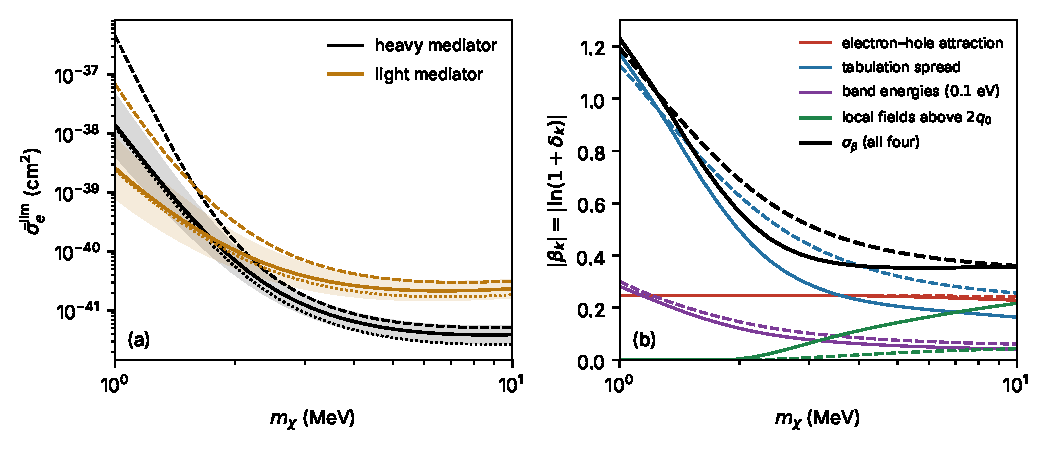
\includegraphics[width=\linewidth]{figures/ch21/fig21_4.pdf}
  \caption{A silicon electron-recoil limit with its theory band. Search: \SI{1}{kg.yr}, every event with at least one pair ($\omega \ge \SI{1.17}{eV}$), no event observed, no background, classical \SI{90}{\percent} limit $N_{90} = 2.303$; standard halo, $\rho_\chi = \SI{0.3}{GeV.cm^{-3}}$. (a) Nominal limit (solid) from the random-phase loss function with local fields of the Knapen--Kozaczuk--Lin tables, whose scissor sets the bands at the measured gap at zero temperature, the band \cref{eq:21.4-band} of the nominal limit (shaded), the profiled limit (dashed; Neyman construction with the nuisance parameter at its conditional best fit, $\ee^{\sigma_\beta^2N_{90}}$) and the limit at the random-phase level without local fields (dotted), for a heavy (black) and a light mediator (ochre). (b) Sensitivities $|\beta_k|$ of the four uncertainties of \cref{we:10-band3}, heavy (solid) and light mediator (dashed). The attraction template is $\delta_{\mathcal{X}} = +0.28$ for $\omega \le \SI{10.5}{eV}$ and zero above, which overstates it above \SI{3}{MeV}, where the compensating weight of the $f$-sum rule enters the window. The other three are the tabulation spread (ratio of the independent-particle rates of the Essig et al.\ and Knapen--Kozaczuk--Lin tables), band energies shifted by \SI{0.1}{eV}, and the random-phase value in place of local fields above $2q_0 = \SI{7.46}{keV}$. Black: their quadrature sum $\sigma_\beta$. Below \SI{1}{MeV} the first energy bins of one table make the spread unreliable. Above \SI{10}{MeV} the momentum range of the other, \SI{22.5}{keV}, truncates the heavy-mediator rate.}
  \label{fig:21-band}
\end{figure}

\begin{workedexample}{The band of a silicon limit from the random-phase level}\label{we:21-rpaband}
Take $\mchi = \SI{3}{MeV}$, a heavy mediator, \SI{1}{kg.yr} of silicon, a one-pair threshold, no event and no background, so that $N^{\mathrm{up}} = N_{90} = 2.303$ and $\sigmae^{\mathrm{lim}} = N_{90}\times\SI{e-37}{cm^2}/\mathcal{R}$, with $\mathcal{R}$ the rate per kilogram-year at $\sigmae = \SI{e-37}{cm^2}$ (\cref{eq:1.5-limit}). The tables place the conduction bands at the measured gap of \SI{1.17}{eV} at zero temperature, and the rate is counted from it (\cref{sec:10.10}).

\emph{The random-phase level.} With the random-phase loss function of the tables, $\mathcal{R} = \num{2.494e4}$ and $\sigmae^{\mathrm{lim}} = \SI{9.23e-42}{cm^2}$.

\emph{The computed step.} The local fields have been computed, and they move the central value, not the band. They lower the rate to \num{1.855e4}, a factor 1.345, and the nominal limit is $\SI{1.24e-41}{cm^2}$.

\emph{The band.} The four uncertainties of \cref{we:10-band3} have, by \cref{eq:21.4-beta} with one bin, $\beta_{\mathcal{X}} = -0.247$ (attraction), $-0.289$ (tabulation spread), $+0.078$ (band energies) and $-0.064$ (local fields above $2q_0$). Their quadrature sum is $\sigma_\beta = 0.393$, and \cref{eq:21.4-band} gives
\begin{equation*}
  \SI{8.38e-42}{cm^2} \le \sigmae^{\mathrm{lim}}(\vartheta) \le \SI{1.84e-41}{cm^2} .
\end{equation*}
The attraction and the tabulation spread carry \SI{93}{\percent} of $\sigma_\beta^2$. Taken one at a time to $\vartheta_k = \pm1$, the four move the limit by factors of 1.28, 1.34, 1.08 and 1.07. The random-phase limit lies in the lower part of the band, at 0.74 of the nominal value against the lower edge at 0.675.

\emph{The profiled limit.} With no events \cref{eq:21.4-profile} is exact, the factor is $\ee^{\sigma_\beta^2N_{90}} = 1.427$, and $\sigmae^{\mathrm{lim,p}} = \SI{1.77e-41}{cm^2}$.

\emph{The detector.} Suppose the efficiency is calibrated to \SI{10}{\percent}, a normalization with $\beta = -\ln 1.10 = -0.095$. Then $\sigma_\beta = 0.404$, the band widens from a factor 1.481 to 1.498, and the profiled factor grows from 1.427 to 1.457. At this calibration the detector adds about one percent to the band and two percent to the profiled limit.
\end{workedexample}

\subsection{One-sided nuisance parameters and excluded cells}\label{sec:21.4-onesided}

A template whose sign is known calls for a constraint that respects it, $\vartheta_k \ge 0$ with the weight $\ee^{-\vartheta_k^2/2}$ on that side, a half-normal constraint. The cost of a half-normal constraint depends on the direction in which the template moves the signal. If $\vartheta_k > 0$ raises the signal, so that $\beta_k < 0$, the statistic at fixed nuisance parameters, \cref{eq:D.47-tfix}, increases with $\vartheta_k$ at every cross-section, and so does the constraint term. The profile then sets $\vartheta_k = 0$ at every cross-section, the parameter costs nothing, and the limit at $\vartheta_k = 0$ is the conservative end of its band. The attraction of \cref{we:21-rpaband} is of this kind: it raises the rate near the gap in every calculation of \cref{sec:10.5}. Only the three other nuisance parameters, with $\sigma_\beta = 0.306$, are then profiled: the profiled factor falls from 1.427 to 1.240 and $\sigmae^{\mathrm{lim,p}} = \SI{1.54e-41}{cm^2}$. The attraction can only strengthen the limit, by 1.28 at $\vartheta_{\mathcal{X}} = 1$. If $\vartheta_k > 0$ lowers the signal, the unconstrained minimum of the profile already lies at $\vartheta_k > 0$, since data without an excess prefer less signal, and the one-sided constraint costs as much as a two-sided one. Linear spin-wave theory, for example, overstates the one-magnon weight of NiO by an estimated $\Delta S/|\vect{S}| = \SI{7.8}{\percent}$ (\cref{sec:14.1}), and that template, of known sign, lowers the signal. Both statements need the template to have one sign in every bin and the bins to be free of excess, so that every weight $a_j$ is positive.

Some cells of the $(\vect{q},\omega)$ plane have no controlled central value, and a limit can be set without them. Removing nonnegative signal from bins without an excess lowers the statistic at every cross-section, so the limit can only rise (\cref{app:D.47}); for one bin it rises by $1/(1 - f)$, with $f$ the removed share. Near the pair-breaking edge of aluminum the conserving loss function changes with the mean free path by more than \SI{10}{\percent} below $y = \omega/\Delta_{\mathrm{BCS}} = 3$, and those energies are excluded (\cref{sec:15.2-nuisance}). At \SI{1}{keV} with a light mediator they hold \SI{20}{\percent} of the rate for the bulk gap and \SI{37}{\percent} for the film gap (\cref{we:15-alrate}), and excluding them weakens the limit by 1.25 and 1.59. For a crystal with a mean free path of at least \SI{10}{\micro m} the clean loss function holds there, and the cells can be restored. The silicon Migdal rate has a region of this kind as well: the coherent zero-phonon response between \SI{0.75}{keV} and $2q_{\mathrm{BZ}}$ is not sized (\cref{tab:12-nuisances}). It carries \SI{33}{\percent} of the rate at \SI{2}{MeV} and \SI{7}{\percent} at \SI{3}{MeV}, so excluding it costs factors of 1.49 and 1.08, and below \SI{1}{MeV}, where it carries nearly all of the rate, no Migdal limit survives the exclusion. In a bin with an excess the argument fails, and removing signal there can strengthen a limit; such a bin needs the full likelihood.

\subsection{The dominant uncertainty of each channel}\label{sec:21.4-dominant}

\Cref{tab:21-dominant} reads the uncertainty budgets of the chapters along the other axis and gives, for each channel at a reference point, the rows that dominate its band. The dominant rows are missing calculations or missing data. The silicon electron recoil lacks a finite-momentum Bethe--Salpeter calculation and a converged independent-particle table, the phonon-assisted window its finite-$q$ form factor and pair-channel screening, the Migdal rate its coherent region and off-diagonal local fields, and NiO its anisotropy. The data that are missing are the cold absorption edge of silicon, the background tensor of ZrTe$_5$ and the gap of an aluminum film. Near the edge of every channel the threshold rows dominate: a gap shift of \SI{10}{meV} weakens a silicon limit \SI{0.005}{MeV} above the edge by a factor of 231 (\cref{we:21-gapshift}).
\begin{table}[tbp]
  \caption{Dominant theory uncertainties of the limit in each channel, read from the uncertainty budgets of the channel chapters. Sizes are factors or shifts of the rate, and hence, for one bin, of the limit. Basis as in those tables: ``computed'', ``model'', ``est.''\ (parametric estimate), ``spread'' (published calculations at the same order), ``data'' (spread of measured inputs), ``bound'' (only an inequality is known), ``unsized''. The last column gives the section, table or figure where the rows are treated.}
  \label{tab:21-dominant}
  \centering\scriptsize\setlength{\tabcolsep}{3pt}
  \begin{tabular}{@{}>{\raggedright\arraybackslash}p{0.20\linewidth}>{\raggedright\arraybackslash}p{0.14\linewidth}>{\raggedright\arraybackslash}p{0.40\linewidth}>{\raggedright\arraybackslash}p{0.09\linewidth}>{\raggedright\arraybackslash}p{0.10\linewidth}@{}}
    \toprule
    Channel & Reference point & Dominant uncertainties & Basis & Section \\
    \midrule
    Electron recoil, Si, density coupling & 1--\SI{3.6}{MeV}, heavy mediator; up to \SI{10}{MeV}, light & tabulation spread: $\times3.2$ at \SI{1}{MeV}, $\times1.34$ at \SI{3}{MeV} (heavy), $\times1.29$ at \SI{10}{MeV} (light); band energies \SI{0.1}{eV}: $\times0.75$ at \SI{1}{MeV} & spread & \cref{sec:10.10}; \SI{1}{MeV}: \cref{fig:21-band} \\
    Electron recoil, Si, density coupling & 3.6--\SI{10}{MeV}, heavy mediator & electron--hole attraction $\times1.28$, $\times1.26$ at \SI{10}{MeV} (known sign); local fields above $2q_0$ $\times1.24$ at \SI{10}{MeV} & model; spread & \cref{sec:10.10} \\
    Electron recoil, velocity couplings & \SI{10}{MeV} & density--current cross term: rate at least 16 (independent particles), about 29 (screened) times the static-electron formula & bound & \cref{sec:10.4} \\
    Core electrons, Ge $3d$ & about \SI{30}{MeV} & crystal final states: $3d$/valence 0.07 against 0.69 & bound & \cref{sec:10.6} \\
    Phonon-assisted electron recoil, Si & 0.333--\SI{0.43}{MeV} & finite-$q$ form factor, factor 3; screening relative to the optical calibration, pair channel not sized; cold absorption data, rate $\times9$ at \SI{0.36}{MeV} & est.; unsized; data & \cref{tab:13-nuisances} \\
    Migdal effect, Si & up to \SI{3}{MeV}; above & coherent zero-phonon response from \SI{0.75}{keV} to $2q_{\mathrm{BZ}}$, \SI{33}{\percent} of the rate at \SI{2}{MeV}; off-diagonal local fields, $\times1.2$ to 1.4, lower end not bounded & unsized; model & \cref{tab:12-nuisances} \\
    Nuclear recoil, Si, multiphonon & \SI{30}{MeV}, $\omega_{\mathrm{th}} = \SI{100}{meV}$ & computed phonon frequencies against measured, \SI{0.24}{\percent}; free recoil in place of the crystal response (evaluation error) $-\SI{6.8}{\percent}$ & computed & \cref{sec:11.9} \\
    Polar phonons, GaAs & single phonon & $Z^*/\varepsilon_\infty$: \SI{2}{\percent} from the measured splitting; a semilocal $\varepsilon_\infty$ moves the rate by \SI{37}{\percent} & data; computed & \cref{sec:11.9} \\
    Magnons, NiO & near \SI{3}{MeV}; lightest masses & one-magnon weight high by \SI{7.8}{\percent} (known sign) against the two-magnon continuum, $+\SI{7.3}{\percent}$ at other energies; magnetic anisotropy near the lightest masses & est.; model & \cref{tab:14-nuisances} \\
    Superconductor, Al & \SI{1}{keV}, light mediator & gap of the sensor, bulk against film: $\times1.23$; edge remainder $-2$ to $+\SI{9}{\percent}$; $y < 3$ excluded, $\times1.25$ (bulk) or $\times1.59$ (film) on the limit & data; computed & \cref{tab:15-nuisances} \\
    Dirac material, ZrTe$_5$ & 20--\SI{1000}{keV}, light mediator & background dielectric tensor: reach band $\times2.8$ & data & \cref{we:16-band} \\
    \bottomrule
  \end{tabular}
\end{table}

For the silicon electron recoil at \SI{3}{MeV} two calculations would remove \SI{93}{\percent} of the variance: a finite-momentum Bethe--Salpeter calculation and an independent-particle table that passes the $f$-sum test at small $q$ (\cref{sec:10.10-open}). With the band energies and the local fields above $2q_0$ left, the band of \cref{we:21-rpaband} would shrink from a factor of 1.48 to 1.11.

\section{Combining and recasting limits}\label{sec:21.5}

Two silicon crystals cut from one wafer and read by identical sensors differ by more than two orders of magnitude in their event rate between 3 and \SI{38}{eV}, because one of them is glued to its holder (\cref{sec:19.6-lee}). The lowest pair bins of a charge detector carry a dark rate, charge that leaks across the gap without any deposit (\cref{sec:1.5-quanta}). No model predicts either rate to the accuracy that a background subtraction needs, so the Poisson limit with a known background of \cref{sec:21.4} cannot be applied to them as it stands. A limit is also rarely the last use of a measurement. A second experiment wants to add its exposure to the first, and a later calculation of the response, such as the background screening of a Dirac material (\cref{sec:16.1}), changes the expected signal after the limit has been published. We will set limits that hold for any background, combine searches in one likelihood whose theory nuisances are shared, and derive when a published limit can be recast to a new response without the data.

\subsection{Limits with an unknown background}\label{sec:21.5-unknown}

If part of the background may be unknown, the only expectation that can safely be assumed for it is zero. Counting every observed event as signal then gives the classical limit of \cref{sec:1.5}: the 90 percent upper limit $N_{\mathrm{sig}}^{\mathrm{lim}}$ solves $P(N \le N_{\mathrm{obs}}\,|\,N_{\mathrm{sig}}) = 0.10$ with the Poisson probabilities \cref{eq:1.5-poisson}, which gives 2.303, 3.890, 5.322 and 6.681 for zero to three events. The limit holds whatever the background is. The distribution function $P(N \le n\,|\,\mu)$ falls monotonically with the mean, since its derivative with respect to $\mu$ is $-P(N = n\,|\,\mu)$, so a signal that leaves a probability below 0.10 for so few events leaves even less once a background $N_{\mathrm{bkg}} \ge 0$ is added to it. The price is that every event, background or not, weakens the limit.

Using the shape of the expected signal gives a stronger limit. At fixed $\mchi$ the spectrum $\dd N_{\mathrm{sig}}/\dd E$ in the measured variable $E$ is known up to the factor $\sigmae$, and a background of a different shape crowds its events where the signal is small, typically near threshold. Yellin's maximum-gap method uses this~\cite{yellin2002finding}. Measure each position by the expected signal count below it, $x(E) = \int^E(\dd N_{\mathrm{sig}}/\dd E')\,\dd E'$. In this variable the signal events of any spectrum are spread uniformly with unit density over $[0, N_{\mathrm{sig}}]$, and the size of a gap between two adjacent events, or between an event and an end of the range, is the signal count expected inside it. For a signal-only experiment the probability that the largest gap is smaller than $x$ depends only on $x$ and $N_{\mathrm{sig}}$~\cite[Eq.~(2)]{yellin2002finding}:
\begin{equation}
  C_0(x, N_{\mathrm{sig}}) = \sum_{k=0}^{m}\Bigl[(kx - N_{\mathrm{sig}})^k - k\,(kx - N_{\mathrm{sig}})^{k-1}\Bigr]\frac{\ee^{-kx}}{k!} , \qquad m = \lfloor N_{\mathrm{sig}}/x\rfloor ,
  \label{eq:21.5-C0}
\end{equation}
written in the form that stays finite when $N_{\mathrm{sig}}/x$ is an integer; Yellin's printed form has the factor $1 + k/(N_{\mathrm{sig}} - kx)$ in place of the bracket, which is the same function away from those points. The 90 percent limit is the cross-section at which the observed largest gap has $C_0 = 0.90$. At fixed mass the fraction $g$ of the expected signal inside the largest gap does not depend on $\sigmae$, so $N_{\mathrm{sig}}^{\mathrm{lim}}$ solves $C_0(gN_{\mathrm{sig}}, N_{\mathrm{sig}}) = 0.90$. With no events the only gap is the whole range, $g = 1$. Then only $k = 0$ and $k = 1$ contribute, the $k = 1$ term is $-\ee^{-N_{\mathrm{sig}}}$, and $C_0 = 1 - \ee^{-N_{\mathrm{sig}}}$ recovers $N_{90} = 2.303$ of \cref{eq:1.5-N90}. The method stays valid with any background: added events can only split gaps, never widen them, so the observed largest gap is no larger than the signal alone would have left, and the limit errs on the conservative side.

How much the shape buys depends on where the events fall. One event that leaves 90 percent of the expected signal on one side gives $g = 0.90$ and $N_{\mathrm{sig}}^{\mathrm{lim}} = 2.836$, against 3.890 from counting. The same event in the middle of the signal, $g = 0.5$, gives 7.78, twice the counting limit; the two methods break even at $g = 0.761$. Two events that both lie in the lowest tenth of the expected signal, where a background rising toward threshold would put them, give $g = 0.90$ and again 2.836, against 5.322 from counting, while two events that cut the signal into thirds give 13.8. The maximum gap gains where the background sits apart from the signal and loses heavily where events are spread through it, and since the method is fixed before the data are seen, an experiment chooses it for the background it expects.

When the events are dense, a gap may be the wrong interval. The optimum-interval method generalizes it~\cite[Sect.~III]{yellin2002finding}. Let $C_n(x, N_{\mathrm{sig}})$ be the probability that, in a signal-only experiment, every interval containing at most $n$ events has an expected count no larger than $x$. It too depends only on $x$ and $N_{\mathrm{sig}}$; it is computed by Monte Carlo and equals \cref{eq:21.5-C0} for $n = 0$. We evaluate $C_n$ for the observed events on every interval bounded by events or by the ends of the range, $(N_{\mathrm{obs}} + 1)(N_{\mathrm{obs}} + 2)/2$ intervals, each with its own $n$ and $x$, and take the largest value, $C_{\mathrm{Max}}$. The 90 percent limit is the cross-section at which $C_{\mathrm{Max}}$ equals the value that 90 percent of signal-only experiments stay below, again from Monte Carlo. That calibration accounts for the interval having been chosen after the data were seen. Both methods need an ordered, continuous variable such as a phonon energy. Integer pair counts leave the events of one bin unordered, and for them the binned analog is a Poisson limit per bin, combined as in \cref{sec:21.5-recast}.

Neither method has a likelihood, since the unknown background has none, and so a theory nuisance cannot be profiled in it: \cref{eq:C.14-profile} needs $\mathsf{L}$. A normalization nuisance scales $N_{\mathrm{sig}}$ at fixed shape, and the band it puts on the limit is the envelope, $(1 + \delta_k)^{\pm1}$, of first order in $\delta_k$, where a likelihood would have charged the second-order cost of \cref{eq:21.4-profile}. A tilt also changes the fractions $g$, because the gaps are measured in expected counts, and the limit must be recomputed with the tilted spectrum at $\vartheta_k = \pm1$.

\subsection{Combining searches with shared nuisances}\label{sec:21.5-combine}

The counts of two exposures are independent, so their Poisson likelihoods multiply (\cref{eq:C.14-poisson}). A combination of experiments $X = \mathrm{A}, \mathrm{B}, \dots$ is one likelihood, the product of the single-exposure likelihoods \cref{eq:8.8-like},
\begin{equation}
  \mathsf{L}\bigl(\sigmae, \vartheta, \vartheta^{\mathrm{det}}\bigr) = \prod_X\mathsf{L}^{(X)}\bigl(\sigmae, \vartheta, \vartheta^{\mathrm{det},(X)}\bigr) .
  \label{eq:21.5-comb}
\end{equation}
Every theory nuisance $\vartheta_k$ appears once and acts in every factor, while the detector nuisances $\vartheta^{\mathrm{det},(X)}$, an efficiency, a background normalization or an energy calibration, are one set per experiment with constraints of their own (\cref{sec:21.4}). The theory nuisances are shared because a truncation is a property of the calculation (\cref{sec:8.8}), and every experiment that uses the same computed response inherits the same error. With one $\vartheta_k$ per experiment the profile could pull them in opposite directions and fit a difference between the experiments that no calculation can produce. It also pays the constraint once for each, as if the errors were independent, and so understates the cost of the truncation.

Before the product, the signal of every experiment is recomputed from one response at one truncation label, since published signal models from different codes differ by more than many of the truncations do. The tabulation spread of \cref{sec:21.4-like} enters \cref{eq:21.5-comb} as one more shared nuisance, not as an error of each experiment. Conventions that differ between publications, the local density, the halo parameters and the pair-creation model that turns energy into pair bins, are choices, not uncertainties, and they are removed by the recomputation, not profiled. Every search on Earth sees the same halo, so if its parameters are varied, one set of them acts on all factors, and near the edge they enter only through the combinations of \cref{sec:21.3-degeneracy}. And searches in different materials share the halo and the nuisance of each truncation that is computed the same way for both, with templates $\delta_k$ of their own and one $\vartheta_k$ (\cref{sec:8.8}). The limit is then set from \cref{eq:21.5-comb} as from a single likelihood (\cref{sec:21.4}).

\begin{workedexample}{Combining two silicon exposures}\label{we:21-combine}
Take $\mchi = \SI{10}{MeV}$, a heavy mediator, the standard halo of \cref{sec:1.2} and the one-pair bin of the cascade of \cref{sec:18.3}, the bin that sets the standard-halo limit at this mass in \cref{sec:21.2-iso}. The tabulated silicon response of \cref{sec:10.1} gives $r = \SI{9.14e41}{kg^{-1}.yr^{-1}.cm^{-2}}$ in this bin, that is 0.914 events per kg-year at $\sigmae = \SI{e-42}{cm^2}$. Exposure A has $M_{\mathrm{det}}t_{\mathrm{exp}} = \SI{1}{kg.yr}$, no events and no background. Exposure B has \SI{4}{kg.yr}, three events and a known background of 2.5 events. Both use the same response, which carries one normalization nuisance, $(1 + \delta)^{\vartheta}$ with $\delta = 0.25$, the size of the largest truncations of the silicon rate at \SI{10}{MeV} in \cref{tab:10-nuisances}.

\emph{Construction.} The limit is the Neyman construction of \cref{sec:21.4-like}. For each $\sigmae$ we sum the Poisson probabilities of all outcomes $(N_{\mathrm{A}}, N_{\mathrm{B}})$ up to 60 events each whose statistic \cref{eq:C.14-profile} is at least the observed one, with the nuisance at its conditional best fit $\hat{\hat\vartheta}$ to the observed counts and the constraint term held fixed. The 90 percent limit is the $\sigmae$ at which that probability is 0.10.

\emph{Without the nuisance.} Exposure A alone excludes $2.303/0.914 = \SI{2.52e-42}{cm^2}$, and B alone $\SI{1.14e-42}{cm^2}$; its three events above a background of 2.5 cost less than its fourfold exposure gains. Together they exclude $\SI{0.809e-42}{cm^2}$, 0.32 of A and 0.71 of B. At the combined limit A expects 0.74 signal events and B 2.96.

\emph{One shared nuisance.} With \cref{eq:21.5-comb} and one $\vartheta$ the limit is $\SI{0.897e-42}{cm^2}$, a factor 1.109 above the combination without it. The profile pulls the nuisance to $\hat{\hat\vartheta} = -0.46$, toward less signal, in both factors at once.

\emph{One nuisance per exposure.} Treated as two independent parameters, the nuisances settle at $-0.17$ (A) and $-0.29$ (B), and the limit is $\SI{0.851e-42}{cm^2}$, a factor 1.051. Splitting the nuisance halves its cost, and the limit is too strong by \SI{5}{\percent}. The worst case within one standard deviation, $\vartheta = -1$, would cost the full factor 1.25.

\emph{One exposure.} For A alone the shared construction gives a closed form. With no events only the outcome $N_{\mathrm{A}} = 0$ has a statistic as large as the observed one, so the limit is reached when the profiled expectation $u = N_{\mathrm{nom}}(1 + \delta)^{\hat{\hat\vartheta}}$ satisfies $\ee^{-u} = 0.10$, $u = N_{90}$. The profile condition of \cref{sec:8.8}, $\hat{\hat\vartheta} = -ku$ with $k = \ln(1 + \delta)$, then gives $N_{\mathrm{nom}} = N_{90}\,\ee^{k^2N_{90}}$, a cost of 1.12 for $\delta = 0.25$, which is \cref{eq:21.4-profile} with $\sigma_\beta = k$ and $\mathsf{t}' = 2N_{90}$.
\end{workedexample}

\subsection{Recasting a published limit}\label{sec:21.5-recast}

A published limit $\sigmae^{\mathrm{lim}}(\mchi)$ was computed with the rates $r_j^{\mathrm{pub}}(\mchi)$ per unit cross-section in the bins $j$ of its analysis. A later calculation replaces them by $r_j^{\mathrm{new}}(\mchi)$, and we write the ratio as the recast factor of bin $j$,
\begin{equation}
  K^{\mathrm{rc}}_j(\mchi) = \frac{r_j^{\mathrm{pub}}(\mchi)}{r_j^{\mathrm{new}}(\mchi)} .
  \label{eq:21.5-K}
\end{equation}
If $K^{\mathrm{rc}}_j = K^{\mathrm{rc}}$ in every bin, the correction preserves the shape of the expected signal at each mass. Every expected count is then $N_{\mathrm{sig},j} = \sigmae M_{\mathrm{det}}t_{\mathrm{exp}}r_j^{\mathrm{new}} = (\sigmae/K^{\mathrm{rc}})M_{\mathrm{det}}t_{\mathrm{exp}}r_j^{\mathrm{pub}}$. Any procedure that depends on $\sigmae$ only through the expected counts, which includes a Poisson limit per bin, a profile likelihood over many bins and Yellin's two methods, returns the limit $K^{\mathrm{rc}}\sigmae^{\mathrm{lim}}$. The recast is then exact without the data.

If $K^{\mathrm{rc}}_j$ varies from bin to bin, the correction tilts the expected spectrum, and the recast needs the procedure. One procedure can be recast exactly: a limit defined as the smallest of single-bin limits, $\sigmae^{\mathrm{lim}} = \min_jN_j^{\mathrm{up}}/(M_{\mathrm{det}}t_{\mathrm{exp}}r_j^{\mathrm{pub}})$, with the upper counts $N_j^{\mathrm{up}}$ of the bins published. Replacing $r_j^{\mathrm{pub}}$ by $r_j^{\mathrm{new}}$ in that minimum is the new limit. If only the curve is public, the new limit is still bracketed. Each new single-bin limit is $K^{\mathrm{rc}}_j$ times the old one, and every old one is at least $\sigmae^{\mathrm{lim}}$, so the new minimum is at least $(\min_jK^{\mathrm{rc}}_j)\,\sigmae^{\mathrm{lim}}$. The bin $j^*$ that set the published limit still offers $K^{\mathrm{rc}}_{j^*}\sigmae^{\mathrm{lim}}$, so the new minimum is at most that. A profile likelihood over several bins and the optimum interval have no such form. Their limits depend on how the counts are spread over bins or events and on all the $r_j$ together, and no function of the published curve and the $K^{\mathrm{rc}}_j$ reproduces them. Recasting them needs the binned likelihood, or the event list.

\begin{keyresult}[Recasting a limit to a new response]
With the recast factors \cref{eq:21.5-K}, a published limit $\sigmae^{\mathrm{lim}}(\mchi)$ becomes
\begin{equation}
  \sigmae^{\mathrm{lim,new}}(\mchi) =
  \begin{cases}
    K^{\mathrm{rc}}(\mchi)\,\sigmae^{\mathrm{lim}}(\mchi) & \begin{tabular}[t]{@{}l@{}}if $K^{\mathrm{rc}}_j = K^{\mathrm{rc}}$ for all $j$\\(any procedure),\end{tabular}\\[2pt]
    \min_j N_j^{\mathrm{up}}\big/\bigl(M_{\mathrm{det}}t_{\mathrm{exp}}\,r_j^{\mathrm{new}}(\mchi)\bigr) & \begin{tabular}[t]{@{}l@{}}if the limit is a minimum over bins\\with $N_j^{\mathrm{up}}$ public\end{tabular}
  \end{cases} ,
  \label{eq:21.5-recast}
\end{equation}
and both forms are exact. For a minimum over bins known only through its curve,
\begin{equation}
  \min_jK^{\mathrm{rc}}_j \le \frac{\sigmae^{\mathrm{lim,new}}}{\sigmae^{\mathrm{lim}}} \le K^{\mathrm{rc}}_{j^*} \le \max_jK^{\mathrm{rc}}_j ,
  \label{eq:21.5-bracket}
\end{equation}
with $j^*$ the bin that set the published limit. A correction that varies between bins cannot be recast from the curve of a profile-likelihood or optimum-interval limit.
\end{keyresult}

A minimum over bins carries a cost in confidence. If each of $n$ independent bins is set at 90 percent, the minimum excludes a true signal whenever any one bin does, and it covers with probability $0.9^n$: 0.81 for two bins and 0.73 for three. The union bound of \cref{sec:21.2-program} restores the stated level. A minimum over bins is recastable exactly only with this correction included in the published $N_j^{\mathrm{up}}$.

Halo conventions show both cases of \cref{eq:21.5-recast}. Take a silicon limit at \SI{10}{MeV} with the search of \cref{sec:21.2-iso}: one kg-year, empty one-, two- and three-pair bins of the cascade and $N_j^{\mathrm{up}} = \ln 30$. It was computed with the halo of Essig et al., $v_0 = 230$, $v_{\mathrm{esc}} = 600$, $v_{\mathrm{E}} = \SI{240}{km.s^{-1}}$ and $\rho_\chi = \SI{0.4}{GeV.cm^{-3}}$~\cite[App.~B]{essig2016direct}, and we recast it to the halo of \cref{app:A.8}. The density enters every rate as a factor, $K^{\mathrm{rc}} = 0.4/0.3 = 1.333$ in every bin, and recasts exactly with any procedure. The velocity distribution does not: at fixed density its recast factors are 0.953, 0.903 and 0.866 in the three bins. The old halo, with smaller $v_0$ and $v_{\mathrm{E}}$, has fewer fast particles in its bulk, and the higher bins need faster particles. With the density the factors are 1.271, 1.204 and 1.154. The published limit, \SI{2.93e-42}{cm^2}, was set by the one-pair bin, and the exact recast is \SI{3.72e-42}{cm^2}, a factor 1.271. From the curve alone, with the binding bin unknown, \cref{eq:21.5-bracket} gives 1.154 to 1.271. At \SI{2}{MeV} the factors are 1.156, 1.432 and 4.0 with the density (0.867, 1.074 and 3.0 without it). The higher bins now draw on the tail, which the old halo extends to $v_{\mathrm{max}} = \SI{840}{km.s^{-1}}$ against 794.5; the three-pair bin opens only above \SI{614}{km.s^{-1}}, and the binding one-pair bin gives 1.156.

The same rule decides how far a theory band can be recast. A normalization nuisance has one $\delta_k$ in every bin, and its band moves with the central limit. A tilt or a threshold shift has bin-dependent templates, and its band needs the per-bin limits or the likelihood, as the central value of any other tilted correction does. \Cref{tab:21-recast} sorts the corrections met in this book.

\begin{table}[tbp]
  \caption{Recast factors \cref{eq:21.5-K} of the corrections met in this book, and what a recast from a published curve needs. ``Common'' means the same factor in every bin at fixed $\mchi$, recastable exactly with any procedure. ``Bin-dependent'' means exact only for a single bin or for a minimum over bins with its upper counts public, and bracketed by \cref{eq:21.5-bracket} otherwise.}
  \label{tab:21-recast}
  \centering\small\setlength{\tabcolsep}{4pt}
  \begin{tabular}{@{}p{0.34\linewidth}p{0.20\linewidth}p{0.38\linewidth}@{}}
    \toprule
    Correction & Factor & Recast \\
    \midrule
    Local density $\rho_\chi$ & common & $\rho_\chi^{\mathrm{pub}}/\rho_\chi^{\mathrm{new}}$, exact \\
    Normalization nuisance (\cref{sec:8.8}) & common & $(1 + \delta_k)^{-\vartheta_k}$, exact, band included \\
    Background in the total $\varepsilon$, isotropic Dirac cone (\cref{sec:16.1}) & common & $\varepsilon_{\mathrm{bg}}^2$ for $\sigmae$, $\varepsilon_{\mathrm{bg}}^{1/2}$ for $\zeta$, exact \\
    Halo velocity distribution ($v_0$, $v_{\mathrm{esc}}$, $v_{\mathrm{E}}$) & bin-dependent & higher bins move most; at the edge through $E_{\mathrm{on}}/v_{\mathrm{max}}^2$ (\cref{sec:21.3}) \\
    Screening and local fields, tilt nuisances (\cref{sec:10.10}) & bin-dependent & templates per bin \\
    Gap or threshold shift & bin-dependent & moves the edge, \cref{we:21-gapshift} \\
    Anisotropic background tensor (\cref{sec:16.1-zrte5}) & depends on $\hat{\vect{q}}$ & ratio of event integrals per mass \\
    Relativistic density row of a boosted flux (\cref{sec:10.9}) & depends on speed & rate ratio $R$, limit $\times R^{-1/2}$ \\
    \bottomrule
  \end{tabular}
\end{table}

An exact recast of any procedure needs what its likelihood contains, and a publication that provides it can be reused without approximation: per bin the observed count, the expected background with its covariance, the exposure and efficiency, the response of the detector from deposited energy to bin with its nuisances, and the upper count with its confidence convention; the halo convention and the truncation label of the signal model; and the likelihood itself in machine-readable form.

\subsection{Dirac and boosted-flux recasts}\label{sec:21.5-corrected}

The published reaches of Dirac materials screen the dark-photon field by the Dirac electrons alone, and the total dielectric function adds the background $\varepsilon_{\mathrm{bg}}$ of the remote bands (\cref{sec:16.1}). For an isotropic cone the published loss function is $\varepsilon_{\mathrm{bg}}^2$ times the true one at every $(\vect{q}, \omega)$, and the published absorption rate $\varepsilon_{\mathrm{bg}}$ times the true one (\cref{eq:16.1-ratio}). The factor is common to every bin and every mass, so by \cref{eq:21.5-recast} the corrected reach is the published curve times $\varepsilon_{\mathrm{bg}}^2$ in $\sigmae$, and times $\varepsilon_{\mathrm{bg}}^{1/2}$ in the mixing $\zeta$, since the absorption rate grows as $\zeta^2$. Nothing else multiplies it: the published $|\varepsilon_{\mathrm{pub}}|^2$ already contains the renormalization of the Dirac charge, $|1 + \varepsilon_{\mathrm{D}}/\varepsilon_{\mathrm{bg}}|^{-2}$, with $\varepsilon_{\mathrm{D}}$ the polarization of the Dirac electrons (\cref{sec:16.1,app:D.41}). \Cref{fig:21-dirac-recast}a recasts the ideal material of Hochberg et al., with $\varepsilon_{\mathrm{bg}} = 40$~\cite{hochberg2018detection}. The minimum of its gapped curve, \SI{3.4e-46}{cm^2} near \SI{9}{keV}, becomes \SI{5.4e-43}{cm^2}, as in \cref{we:16-factor}, and at \SI{114}{keV} the gapless curve moves from \SI{5.5e-45}{cm^2} to \SI{8.8e-42}{cm^2}.

\begin{figure}[tbp]
  \centering
  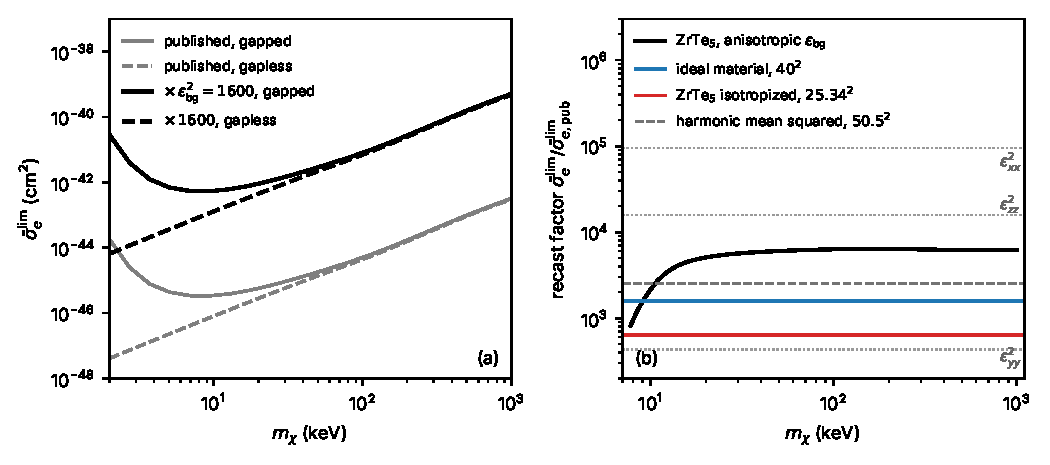
\includegraphics[width=\linewidth]{figures/ch21/fig21_5.pdf}
  \caption{Recasting published Dirac-material reaches to the total dielectric function; light mediator, three events in one kg-year, no background. (a) The ideal Dirac material of Hochberg et al.~\cite{hochberg2018detection} ($v_{\mathrm{D}} = 4\times10^{-4}$, $\varepsilon_{\mathrm{bg}} = 40$, $g_{\mathrm{deg}} = 2$, cutoff \SI{0.2}{keV}): published curves (gray), gapped ($\Delta_{\mathrm{D}} = \SI{2.5}{meV}$, solid) and gapless (dashed), read from the reference's figure. Black: the same curves times $\varepsilon_{\mathrm{bg}}^2 = 1600$, exact for any procedure because the factor is the same at every $(\vect{q},\omega)$. (b) Recast factor, the ratio of the corrected to the published reach, against $\mchi$. Black: the ratio of the published-rule to the total-$\varepsilon$ event integral at each mass for ZrTe$_5$ (\cref{sec:16.1-zrte5}). It uses the anisotropic background tensor $\varepsilon_{\mathrm{bg},ii} = 308.4$, 20.75, 126.1 and the measured-structure row of Geilhufe et al.~\cite{geilhufe2020dirac} ($\Delta_{\mathrm{D}} = \SI{11.8}{meV}$), the book's halo and the rate averaged over orientations of the crystal. Flat lines: $40^2 = 1600$ (blue) and $25.34^2 = 642$ for the isotropized ZrTe$_5$ of Hochberg et al. (red), both exact; the square of the harmonic mean of the tensor, $50.5^2 = 2554$ (gray dashed); the on-axis factors $\varepsilon_{\mathrm{bg},ii}^2 = 431$, $1.6\times10^4$ and $9.5\times10^4$ (gray dotted).}
  \label{fig:21-dirac-recast}
\end{figure}

An anisotropic crystal has no common factor. Its published rule divides each component of the Dirac polarization by its own $\varepsilon_{\mathrm{bg},ii}$, the total dielectric function adds the background along $\hat{\vect{q}}$, and their ratio depends on the direction of $\vect{q}$ and on $(q, \omega)$ (\cref{eq:D.41-ratio}). The published ZrTe$_5$ reach is, however, a single count, three events with no background, and a single bin is the case $n = 1$ of a minimum over bins: the recast is exact once both event integrals are computed at each mass. Their ratio is 5100 to 6400 between \SI{20}{keV} and \SI{1}{MeV} (\cref{fig:21-dirac-recast}b). Toward the threshold it falls, to 2200 at \SI{10}{keV} and 820 at \SI{7.7}{keV}, because only momentum transfers near the $y$ axis, with the lowest threshold, \SI{7.1}{keV}, and the smallest background constant, remain kinematically allowed there, and along that axis the factor is $\varepsilon_{\mathrm{bg},yy}^2 = 431$. No constant reproduces the curve: the square of the harmonic mean of the tensor, the natural isotropic guess, is low by a factor of two to two and a half above \SI{20}{keV} and high near threshold.

A boosted flux changes the counting itself. Dark matter accelerated by cosmic rays acquires its speed through the same coupling that the detector measures, so the flux is proportional to $\sigmae$ and the expected count to $\sigmae^2$, as the published analysis of silicon and germanium states~\cite{liang2025plasmon}. With $N^{\mathrm{up}}$ fixed, a change of the detection rate per particle by a ratio $R$ moves the lower edge of the excluded region by $R^{-1/2}$. For the exact density row of a relativistic particle, \cref{eq:10.9-Drel}, the ratios are those of \cref{sec:10.9-boosted}: the heavy-mediator limit is unchanged, the shift of $\sigmae$ for a massless mediator is below one percent for $\mchi \ge \SI{10}{keV}$, and below about \SI{3}{keV} it is undetermined. Settling it, with the transverse row and its Cherenkov pole included, is the recast that \cref{sec:10.9-open} leaves open and \cref{app:E.16} specifies.

\section{Next targets}\label{sec:21.7}

CsI has a heavy-mediator single-phonon rate per unit mass 3.73 times that of silicon, on elastic constants measured at \SI{4.2}{K}, and 1.56 times that of TeO$_2$, the leader of the eleven crystals ranked in \cref{sec:17.6}. The lead salts have electron-recoil floors up to 4.4 times below germanium's. Neither family was in that pool: no CsI crystal has been read by a phonon sensor at millikelvin temperatures, and a lead compound carries the $^{210}$Pb of its lead, whose $\beta$ spectrum puts some 700 events per kilogram, day and keV below \SI{1}{keV} for every becquerel per kilogram. A ranking of responses answers which crystal gives the most rate per unit mass. An experimentalist choosing the target of the next experiment also needs to know what each leader still has to demonstrate, which measurement would change the order, and on what the probabilities rest. We combine the response-level rankings of \cref{sec:17.6} with the pair energies of \cref{sec:18.4}, the readout verdicts of \cref{sec:20.5} and the internal backgrounds of the crystals into a guide with one row per channel, \cref{tab:21-guide}.

\subsection{Candidate pools and detector readiness}\label{sec:21.7-pools}

The \emph{full pool} holds 42 crystals: 23 of the 24 crystals of the target table of Griffin and collaborators~\cite[Table~I]{griffin2020multichannel}, all but InSb, the three SiC polytypes, and the targets of the preceding chapters that have the inputs of at least one figure of merit. Four requirements decide whether a crystal can be the target of a cryogenic experiment now. The crystal operates at millikelvin temperatures after thermal cycling, without a phase transition between \SI{300}{K} and \SI{10}{mK} and without absorbing water from the air. At least \SI{1}{g} of detector-grade crystal can be grown, or an array of instrumented crystals of at least \SI{0.1}{g} each adds up to a gram. A sensor has been read on its surface at millikelvin temperatures. And its intrinsic rate below \SI{1}{keV} is at most one event per kilogram, day and keV. A crystal for which all four are documented is a \emph{survivor}. A crystal for which one or more is not documented, though none is shown to be impossible, is a \emph{conditional survivor}. Only positive evidence removes a crystal from the full pool. That evidence exists for two candidates, KTaO$_3$ and InSb, whose natural $^{40}$K and $^{115}$In give intrinsic rates far above the fourth requirement (\cref{sec:21.7-backgrounds}).

The survivor pool is the eleven crystals of \cref{sec:17.6}: silicon, germanium, GaAs, diamond, sapphire, LiF, NaF, CaWO$_4$, TeO$_2$, Li$_2$MoO$_4$ and $\gamma$-LiAlO$_2$. The other 31 are conditional. Membership records what has been documented for a crystal, not its physics, and it changes with one demonstration. GaAs entered when a \SI{4.3}{g} crystal was operated at about \SI{10}{mK} with a thermistor readout~\cite{melchiorre2025first}. Diamond entered through the array route: two crystals of \SI{0.175}{g} each, grown by chemical vapor deposition and read by tungsten transition-edge sensors, one with a threshold of \SI{16.8}{eV}~\cite{angloher2023light}. Six such crystals make a gram, each with its own readout channel and threshold, and their surface-to-volume ratio is $(1/0.175)^{1/3} = 1.79$ times that of a single gram crystal, which raises any surface background in proportion. The survivor leader of a channel is the best target that the record supports today. The full-pool leader says what a demonstration would gain: if it differs from the survivor leader, the missing demonstration of the full-pool leader is worth as much as its lead.

The rankings of the full pool use the method and widths of \cref{sec:17.6} unchanged. For the conditional crystals the gaps are those of the target table, a room-temperature gap shifted upward by an amount drawn uniformly between 0.03 and \SI{0.10}{eV}, and the SiC gaps are room-temperature values of the SiC target table~\cite[Table~I]{griffin2021sic}. Their elastic tensors are computed ones from the same database as in \cref{sec:17.6}~\cite{choudhary2018elastic}, with the width 0.086, except two that are measured: aluminum at zero temperature and CsI at \SI{4.2}{K}~\cite{vallin1964elastic}, width 0.02. Their polar band integrals come from \cref{eq:11.2-diatomic} with computed Born charges, $\varepsilon_\infty$ and highest optical energies~\cite[Table~I]{griffin2020multichannel}, or from the measured dielectric constants of the SiC polytypes~\cite[Table~I]{griffin2021sic}.

We add one channel that \cref{sec:17.6} did not rank: the threshold in quanta, measured by the pair energy $\varepsilon_{\mathrm{eh}}$. A lower pair energy turns the same deposit into more pairs and puts the one- and two-pair bins of a charge readout at lower energy (\cref{sec:18.3}). Where a pair energy has been measured, the guide uses the measurement: silicon \SI{3.749}{eV} at \SI{123}{K}~\cite{rodrigues2021absolute}, GaAs about \SI{4.2}{eV} at room temperature~\cite[Fig.~1]{nielsen2026first} raised by $1.70 \times \SI{0.10}{eV}$ for the shift of its gap on cooling (the slope $\partial\varepsilon_{\mathrm{eh}}/\partial\Eg$ of the cascade at fixed constant, \cref{sec:18.4}), diamond and the SiC polytypes as in \cref{fig:18-limit-c}, and germanium as discussed below. For every other crystal the pair energy is the estimate of the cascade of \cref{sec:18.4} at the tabulated gap and highest optical phonon energy. Inside the validated range of \cref{sec:18.4-range} we give it a logarithmic width 0.105, the root mean square of the residuals of the seven crystals with measured values; outside it the width is doubled to 0.21, a convention, since no measurement anchors these crystals.

Germanium has no pair energy measured directly at millikelvin temperatures. Its pair energy at \SI{77}{K} is \SI{2.96}{eV}, the value \cref{sec:18.4} tests the cascade against. The one value quoted at millikelvin temperatures, $(3.37 \pm 0.01)$~eV, comes from a fit by Wei, Wang and Mei to the ratio of phonon to ionization energy measured in EDELWEISS detectors as a function of bias, $E_{\mathrm{p}}/E_{\mathrm{Q}} = a + eV_{\mathrm{bias}}/\varepsilon_{\mathrm{eh}}$, in which the relative conversion efficiency $a = 0.85$ of primary and Luke phonons is fitted together with $\varepsilon_{\mathrm{eh}}$~\cite[Sect.~2.1.4]{wei2016average}. The value rests on the assumption that one constant $a$ describes the phonon collection at every bias, the quantity whose detector dependence \cref{sec:20.5} found open. We use 3.37~eV with the width 0.015 of the spread between this fit and their resolution-based value of 3.32~eV. Either value puts germanium ahead of silicon.

Every probability in the guide is conditional on the provenance widths of \cref{sec:17.6-widths}. The guide reads every row at independent method errors, $r_{\mathrm{mat}} = 0$ in \cref{eq:17.6-zmethod}, and prints the value at $r_{\mathrm{mat}} = 1$ beside it.

\subsection{The guide to next targets}\label{sec:21.7-guide}

\Cref{tab:21-guide} is the guide. The survivor leaders and their values, except in the pair-energy row, are those of \cref{tab:17-rank}.

\begin{table}[tbp]
  \caption{The guide to next targets. Leaders of the full pool (42 crystals) and of the survivor pool (eleven crystals, \cref{sec:21.7-pools}). Full-pool leader: median with 68\% interval, and probability of ranking first at independent method errors with the value at $r_{\mathrm{mat}} = 1$ in parentheses; the values of the survivor leaders are in \cref{tab:17-rank}. Every probability is conditional on the provenance widths of \cref{tab:17-widths} and on the widths of the pair energies stated in \cref{sec:21.7-pools}; it is not the probability that a crystal is the better target. Missing demonstration: the requirements of \cref{sec:21.7-pools} not documented for the leader. Edges at $\omega_{\mathrm{th}} = \SI{1}{meV}$; $v_{\mathrm{max}} = 2.650\times10^{-3}$.}
  \label{tab:21-guide}
  \centering\scriptsize\setlength{\tabcolsep}{3pt}
  \begin{tabular}{@{}>{\raggedright\arraybackslash}p{0.14\linewidth}>{\raggedright\arraybackslash}p{0.24\linewidth}>{\raggedright\arraybackslash}p{0.12\linewidth}>{\raggedright\arraybackslash}p{0.22\linewidth}>{\raggedright\arraybackslash}p{0.20\linewidth}@{}}
    \toprule
    Channel; figure of merit & Full-pool leader & Survivor leader & Missing demonstration & Deciding measurement \\
    \midrule
    Electron-recoil floor; $2\Eg/v_{\mathrm{max}}^2$ & PbSe, \SI{0.0484}{MeV} [0.0479, 0.0489]; 1.000 (1.000); PbTe and PbS next & Ge & lead salts: a crystal of at least \SI{0.1}{g} read at mK; $^{210}$Pb below \SI{1.38}{mBq} per kg of compound & $^{210}$Pb activity of the lead available for growth; low-temperature gap of GaSb \\
    Threshold in quanta; $\varepsilon_{\mathrm{eh}}$ & PbTe, \SI{1.52}{eV} [1.24, 1.87]; 0.482 (1.000); one tier with PbSe (0.414) and PbS (0.102) & Ge, \SI{3.37}{eV} [3.32, 3.42]; then Si 3.75, GaAs 4.37 & lead salts: as above; one measured pair energy of a lead salt & pair energy of germanium measured at mK with the phonon collection calibrated separately \\
    Heavy-mediator single phonon; $c_{\mathrm{NR1}}(\mathrm{Si})/c_{\mathrm{NR1}}$ & CsI, 3.73 [3.65, 3.80]; 0.962 (0.976); measured \SI{4.2}{K} tensor & TeO$_2$, computed tensor & CsI: an encapsulated crystal cycled to mK and read by a phonon sensor & measured elastic constants of TeO$_2$; measured $^{123}$Te capture rate \\
    Nuclear edge; $m_{\mathrm{min}}^{\mathrm{ac}}$ with $c_{\mathrm{LA,max}}$ & no resolved leader: h-BN, \SI{2.95}{keV} [2.72, 3.21]; 0.656 (0.728); one tier with diamond (0.181), polyethylene (0.119), cubic BN (0.043) & diamond, measured tensor & diamond: six crystals of \SI{0.175}{g}, each with its own threshold and low-energy-excess rate, and a phonon threshold near \SI{1}{meV} (shown: \SI{16.8}{eV}); h-BN: mass, mK and readout & measured elastic constants of h-BN, polyethylene and cubic BN \\
    Polar rate; $\mathcal{I}_{\mathrm{pol}}/\rho_T$ & LiF, 19.0 [15.5, 23.3]; 0.918 (0.931) & LiF & LiF: the $^6$Li neutron-activation background, not measured & measured $\varepsilon_0$ and Born charge of LiF at low temperature \\
    Polar reach; $2\omega_{\mathrm{L}}/v_{\mathrm{max}}^2$ & CsI, \SI{2.85}{keV} [2.71, 2.99]; 0.996 (1.000); computed $\omega_{\mathrm{L}}$ & GaAs, measured $\omega_{\mathrm{L}}$ & GaAs: a threshold below its longitudinal phonon, \SI{36.35}{meV}; CsI: as above & low-temperature longitudinal optical frequency of CsI \\
    Migdal; pole factor times $X_{\mathrm{pole}}$ & no resolved leader: NaCl 0.498 (1.000) & no resolved leader: NaF 0.315 (1.000) & -- & $L(\vect{k},\omega)$ of every candidate \\
    \bottomrule
  \end{tabular}
\end{table}

Germanium leads both electron-recoil rows among the survivors, the floor on its measured low-temperature gap and the threshold in quanta with 1.11 times fewer electron volts per pair than silicon. Its lead in quanta holds on the \SI{77}{K} value as well, which is lower still, so the 50~mK fit affects the number and leaves the order unchanged. In the full pool the lead salts lead both rows. PbSe has the lowest floor, on a gap measured at low temperature (\cref{fig:17-rank-floor}). In quanta PbTe, PbSe and PbS share the leading tier. Their pair energies are cascade estimates for crystals whose phonon strengths $\lambda_{\mathrm{AB}}$, the dimensionless ratio of phonon emission to impact ionization in the cascade (\cref{sec:18.4-range}), lie between 230 and 1160, two orders of magnitude outside its validated range, so the tier is real only under the width convention. GaSb, whose estimate lies at the edge of that range, beats germanium's measured value with probability 0.83. At $r_{\mathrm{mat}} = 1$ the three estimates of the lead salts share their error and PbTe ranks first in every draw. No lead salt has been operated at millikelvin with a phonon or charge readout, and every one carries $^{210}$Pb in its bulk (\cref{sec:21.7-backgrounds}).

The heavy-mediator rows separate the two pools most clearly. TeO$_2$ leads the survivors on a computed tensor. CsI, a conditional survivor, leads the full pool on elastic constants measured at \SI{4.2}{K}, from which the Christoffel problem of \cref{sec:17.6} gives $c_{\mathrm{NR1}} = \SI{2.404}{km.s^{-1}}$ and the figure of merit $8.956/2.404 = 3.73$ times silicon. It is ahead of Bi$_2$Se$_3$ and NaI, both computed, with probabilities 0.978 and 0.985, and of TeO$_2$ by a factor 1.56 in the medians, larger than any width. A colder, denser cell, at most \SI{4.5}{\percent} denser than the room-temperature one, raises the figure of merit to 3.81. Against silicon the ratio of the figures of merit gives the ratio of the rates to \SI{10}{\percent} from \SI{97}{keV} up to the zone cap of CsI at \SI{0.32}{MeV} (\cref{fig:17-window}). On its computed highest optical energy, \SI{10.0}{meV}, CsI also leads the polar reach, 3.64 times below GaAs. The same softness gives CsI a poor nuclear edge: from $c_{\mathrm{LA,max}} = \SI{2.46}{km.s^{-1}}$ the edge is \SI{23.1}{keV}, last of the eleven crystals ranked in that row. Two of the four requirements are documented for CsI: crystals far above a gram are grown, and neither caesium-133 nor iodine-127 is radioactive. CsI is slightly hygroscopic, and its operation at millikelvin temperatures after thermal cycling, with a sensor read on it, is not documented. Its entry needs an encapsulated crystal that survives cycling to millikelvin temperatures and a phonon sensor that reads it, deposited on the crystal or on a carrier in thermal contact with it. Its lead then depends on its background: it tolerates $1.56^2 = 2.44$ times TeO$_2$'s background rate density in a background-limited search (\cref{sec:21.7-backgrounds}), and the cosmogenic iodine and caesium isotopes, whose production rates have not been measured for CsI, set that rate.

In the nuclear edge the stiffest crystals lead: diamond leads the survivors on its measured tensor, but in the full pool it shares the leading tier with h-BN, polyethylene and cubic BN, and no leader is resolved. h-BN and polyethylene owe their place to one stiff direction, in the hexagonal plane and along the chains, and their tensors are computed; they reach their edges only for momentum along those directions. LiF leads the polar rate in both pools. The polar reach goes the other way, to soft polar lattices: GaAs among the survivors on its measured longitudinal frequency, CsI in the full pool on a computed one.

The Migdal figure of merit has no leader at independent errors in either pool, for the reason found in \cref{sec:17.6-correlation}, and the light-mediator single-phonon rate ranks no crystals (\cref{tab:17-rank}).

By \cref{sec:20.5}, a leader of an electron-recoil row is read by its charge, through the cascade distribution $P(N_{\mathrm{eh}})$ of \cref{chap:18}, and a leader of a phonon row by its heat, through a collection efficiency that only the detector's kernels fix. A superconducting absorber is read by quasiparticles, with the yield $2\Delta_{\mathrm{BCS}}/E$ below $4\Delta_{\mathrm{BCS}}$ and 0.59 above (\cref{sec:20.4}).

The theory band of a limit (\cref{sec:21.4}) and the ranking of targets answer different questions. An uncertainty that multiplies the rates of every crystal by the same factor, such as the halo or a shared response approximation, moves every limit and no ranking. A ranking moves only through the inputs that differ between crystals, which is why the provenance widths, and not the bands of \cref{tab:21-dominant}, set the probabilities of the guide.

\subsection{Absorption and unranked channels}\label{sec:21.7-other}

Absorption has leaders only mass by mass, the best reach of each decade of \cref{tab:17-abs-decades}. For the dark photon they are zeros of $\varepsilon_1$, where the screening ceiling $L \le 1/(2|\varepsilon_1|)$ is highest: the longitudinal phonon of GaAs, the highest polar branch of sapphire and the plasmon of silicon. All three are survivors. For the axion-like particle with its electron coupling the magnon line of YIG leads from 10~\si{\micro eV} to a meV and clean aluminum from 0.36 to \SI{10.9}{meV}. Neither is a survivor, since the YIG spheres are of millimeter size and no bulk aluminum absorber has been read. The aluminum reach rests on direct pair breaking by the spin current (\cref{sec:15.4-spin}). It holds for a mean free path well above the size of a pair, 1.6 to \SI{2.4}{\micro m}, which only bulk high-purity crystals reach; in a \SI{50}{nm} film the spin channel and the published mapping give comparable reaches.

Magnons, superconductors and the special targets of \cref{chap:16} have no ranking, because no second candidate has the inputs of the same figure of merit. The edge of NiO is set by the magnetic anisotropy that the Heisenberg model leaves out (\cref{sec:14.1}). The scattering rate of aluminum depends more on the gap and mean free path of the absorber actually used than on the choice among loss functions (\cref{sec:15.2}). The one-loop expansion parameter of ZrTe$_5$ is about one, so its rate has no controlled theory at that half-gap (\cref{sec:16.1}). NiO and ZrTe$_5$ lack a gram-scale crystal read at millikelvin temperatures, and aluminum a quasiparticle readout of a bulk absorber.

\subsection{Internal radioactive backgrounds}\label{sec:21.7-backgrounds}

Every figure of merit in the guide ranks signal rates, and a background enters the ranking through a tolerance. Let $b$ be the background rate density in a region of width $\Delta E$. If a search is background limited, the signal must exceed a fixed number of standard deviations of the background count, and its exclusion limit scales as $(b\,\Delta E)^{1/2}/\mathcal{R}$. At the systematics floor, where the background is subtracted only to a fixed fraction, the limit scales as $b\,\Delta E/\mathcal{R}$. Crystal $A$ then keeps its lead over $B$ if $b_A/b_B < (\mathcal{R}_A/\mathcal{R}_B)^2$, or $b_A/b_B < \mathcal{R}_A/\mathcal{R}_B$ at the floor. TeO$_2$ leads CaWO$_4$ in the heavy-mediator rate by 1.22, so it tolerates 1.48 times CaWO$_4$'s background in a background-limited search and 1.22 at the floor. LiF tolerates 3.63 times NaF's background in the polar rate. A lead that rests on a rate factor of order one is reversed by a background ratio of order one. The edges are kinematic and do not move with $b$, but the sensitivity just above them does.

The background that belongs to the crystal itself, and that no shield removes, comes from radioactive nuclei inside it. A $\beta$ emitter spread uniformly through a crystal much larger than the range of its electrons deposits the whole kinetic energy of the electron, and the antineutrino escapes. The spectrum of deposits is then the $\beta$ spectrum, normalized to the activity $\mathcal{A}_{\mathrm{act}}$ per unit mass. For an allowed transition with endpoint $Q_\beta$ it is
\begin{equation}
  n_\beta(T) \propto p_eE_e(Q_\beta - T)^2\,\frac{2\pi y_{\mathrm{S}}}{1 - \ee^{-2\pi y_{\mathrm{S}}}} , \qquad y_{\mathrm{S}} = \frac{\alpha Z_{\mathrm{d}}E_e}{p_e} ,
  \label{eq:21.7-beta}
\end{equation}
with $T$ the kinetic energy of the electron, $E_e = T + m_e$ and $p_e$ its total energy and momentum, $Z_{\mathrm{d}}$ the charge of the daughter nucleus, and the last factor the nonrelativistic Fermi function, which accounts for the Coulomb attraction of the daughter. A unique $n$-th forbidden transition carries in addition the shape factor $\sum_{k=0}^{n}p_e^{2k}q_\nu^{2(n-k)}/[(2k+1)!\,(2n-2k+1)!]$, with $q_\nu = Q_\beta - T$ the momentum of the antineutrino. As $T \to 0$ the factor $p_e$ cancels against the $1/p_e$ of the Fermi function, so the spectrum tends to a constant: the low-energy end of a $\beta$ spectrum is flat. The rate density below \SI{1}{keV} is therefore $\mathcal{A}_{\mathrm{act}}f_\beta$ per keV, with $f_\beta$ the fraction of the spectrum below \SI{1}{keV}. With $Q_\beta = \SI{18.59}{keV}$ for tritium~\cite{iaea2026livechart}, \cref{eq:21.7-beta} gives $f_\beta = 0.0892$. Cosmogenic tritium in silicon is produced at sea level at 124 atoms per kilogram and day. It then contributes 0.169 events per kilogram, day and keV below \SI{1}{keV} after a hundred days and 11.0 at saturation (\cref{app:E.27}). In germanium, at 82 atoms per kilogram and day~\cite{armengaud2017measurement}, the two values are 0.112 and 7.31. Cosmogenic activation is reducible: growth, fabrication and storage underground, and in silicon the out-diffusion of hydrogen, lower it. The other cosmogenic nuclides decay by electron capture, and their L and M lines near 1 and \SI{0.1}{keV} enter the sub-keV region through their L and M fractions. Their production rates have been measured for silicon and germanium~\cite{saldanha2020cosmogenic,armengaud2017measurement} and not for the other survivors.

A lead compound carries a background that no exposure history changes. Its lead contains $^{210}$Pb, half-life 22.2 years, which decays to $^{210}$Bi and, five days later, to $^{210}$Po; in equilibrium the three activities are equal~\cite{iaea2026livechart}. In 84 percent of its decays $^{210}$Pb feeds the level of $^{210}$Bi at \SI{46.5}{keV}, with a $\beta$ endpoint of \SI{17.0}{keV}. The de-excitation of that level, a photon or conversion electrons with their X-rays, is absorbed in the bulk, so these decays deposit at least \SI{46.5}{keV} and never fall below \SI{1}{keV}. The other 16 percent go to the ground state, with $Q_\beta = \SI{63.5}{keV}$. For a daughter as heavy as $^{210}$Bi, $Z_{\mathrm{d}} = 83$, the nonrelativistic factor of \cref{eq:21.7-beta} is crude, and we use instead the traditional relativistic Fermi function of a point charge, with the prefactor 4, evaluated at the nuclear radius $r_A = 1.2A^{1/3}\,\mathrm{fm}$~\cite[Eq.~(6)]{hayen2018high},
\begin{equation}
  F_{\mathrm{Fermi}}(Z_{\mathrm{d}}, T) = 4\,(2p_er_A)^{2(\gamma_{\mathrm{d}} - 1)}\,\ee^{\pi y_{\mathrm{S}}}\,\frac{|\Gamma(\gamma_{\mathrm{d}} + \ii y_{\mathrm{S}})|^2}{\Gamma(1 + 2\gamma_{\mathrm{d}})^2} , \qquad \gamma_{\mathrm{d}} = \sqrt{1 - Z_{\mathrm{d}}^2\alpha^2} ,
  \label{eq:21.7-fermi}
\end{equation}
in place of the last factor of \cref{eq:21.7-beta}, with $y_{\mathrm{S}}$ as there. It gives $f_\beta = 0.0445$. The $^{210}$Bi decay to $^{210}$Po, $Z_{\mathrm{d}} = 84$ and $Q_\beta = \SI{1161}{keV}$, adds $f_\beta = 1.26\times10^{-3}$ with the allowed shape, and the $\alpha$ decay of $^{210}$Po deposits megaelectronvolts. Per becquerel of $^{210}$Pb per kilogram the rate density below \SI{1}{keV} is
\begin{equation}
  \begin{split}
  b_{^{210}\mathrm{Pb}} &= \SI{86400}{s.d^{-1}}\times(0.16 \times 0.0445 + 1.26\times10^{-3})\ \mathrm{keV}^{-1}\times\SI{1}{Bq.kg^{-1}}\\
  &= 724\ \text{per kg, day and keV} .
  \end{split}
  \label{eq:21.7-pb210}
\end{equation}
Of these, 614.7 come from $^{210}$Pb and 109.2, fifteen percent, from $^{210}$Bi. A budget of one event per kilogram, day and keV then needs an activity below \SI{1.38}{mBq} per kilogram of compound: 1.91, 2.23 and \SI{1.60}{mBq} per kilogram of lead in PbSe, PbTe and PbS. The number is an estimate. The relativistic Fermi function raises it by \SI{5}{\percent} over the nonrelativistic 689, mostly through the $^{210}$Bi part, and the first-forbidden transition of $^{210}$Bi, whose shape departs from the allowed one, moves that part further by an amount not computed here. Whether lead of that purity can be obtained and grown into a crystal decides whether the floor of a lead salt is usable, and it is the deciding measurement of the first two rows of \cref{tab:21-guide}.

Primordial nuclei set the only exclusions of the full pool. Natural potassium carries $^{40}$K at \SI{31.7}{Bq} per gram; \SI{89.3}{\percent} of its decays are unique third-forbidden $\beta$ decays with $Q_\beta = \SI{1311}{keV}$~\cite{iaea2026livechart}, for which \cref{eq:21.7-beta} with its shape factor gives $f_\beta = 4.13\times10^{-4}$. KTaO$_3$, \SI{14.6}{\percent} potassium by mass, holds \SI{4.6}{kBq} of $^{40}$K per kilogram and has a $\beta$ rate density of $1.5\times10^5$ per kilogram, day and keV below \SI{1}{keV}. InSb holds \SI{121}{Bq} of $^{115}$In per kilogram, a fourth-forbidden non-unique emitter with $Q_\beta = \SI{497}{keV}$ whose shape is not known; bracketed between the allowed and the unique fourth-forbidden shapes, its rate density lies between $4.8\times10^3$ and $3.9\times10^4$. Both exceed the budget by more than three orders of magnitude, and since only isotopic depletion removes a primordial nucleus, both leave the pool. TeO$_2$ is the opposite case. Its $^{123}$Te is known only to have a half-life above $9.2\times10^{16}$ years~\cite{iaea2026livechart}, so its electron captures are bounded by 693 per kilogram and day, and by the same number per keV if all of them fell in one keV below \SI{1}{keV}. The bound does not decide whether TeO$_2$ meets the budget, and its radioactivity entry stays conditional on a measured capture rate.

Gamma lines of nuclei inside the crystal add a Compton continuum. A photon of energy $E_\gamma$ that scatters once and leaves deposits the electron's recoil energy $T$, and at $T \to 0$ the Klein--Nishina cross-section per electron tends to
\begin{equation}
  \frac{\dd\sigma_{\mathrm{C}}}{\dd T}\bigg|_{T \to 0} = \frac{2\pi r_{\mathrm{cl}}^2m_e}{E_\gamma^2} ,
  \label{eq:21.7-compton}
\end{equation}
with $r_{\mathrm{cl}}$ the classical electron radius; at \SI{1}{keV} the full form for the \SI{1461}{keV} line of $^{40}$K differs from it by $2\times10^{-4}$, and its value there is \SI{1.20e-28}{cm^2.keV^{-1}}. The rate density below \SI{1}{keV} is the photon emission rate times $\nd_e\bar\ell_{\mathrm{esc}}\,\dd\sigma_{\mathrm{C}}/\dd T$ in the thin-target limit, with $\nd_e$ the electron density and $\bar\ell_{\mathrm{esc}}$ the mean path from a point inside the crystal to its surface. For a cube of side $L$ the path from a uniformly distributed interior point in an isotropic direction averages $0.448\,L$, not the mean chord $4V/S = 0.667\,L$ of rays crossing the cube from outside. With $\nd_e = \SI{2e24}{cm^{-3}}$ and $L = \SI{5}{cm}$ a fraction $5.4\times10^{-4}$ of the \SI{1461}{keV} photons deposits in each keV below \SI{1}{keV}. The continuum is flat at low energy like the $\beta$ spectrum, and for an emitter with a $\gamma$ line it adds to the $\beta$ deposits.

\subsection{Open problems}\label{sec:21.7-open}

Three missing inputs limit the guide: the loss functions of the survivors, measured elastic constants, and internal-background rates. The first is the loss function $L(\vect{k},\omega)$ of every survivor near its gap at momenta up to a few keV. Without it the Migdal figure of merit is known only between the plasmon-pole and gap-weighted limits, the prior $X_{\mathrm{pole}}$ stands in for the interband weight, and the row has no resolved leader in either pool.

The second is elastic constants. TeO$_2$, the survivor leader of the heavy-mediator row, and h-BN, polyethylene and cubic BN, which share the leading tier of the full-pool nuclear edge, rest on computed tensors. These carry the method offset that \cref{sec:17.6-correlation} found for the computed family, \SI{4.9}{\percent} on average for silicon, germanium and diamond. For CsI the density of the cold cell is missing.

The third is the internal backgrounds, which the guide has only estimated. The sub-keV rates of $\beta$ emitters use allowed or unique shapes, which are crude for the first-forbidden decay of $^{210}$Bi and unknown for $^{115}$In; the $^{210}$Pb activity of lead that can be grown into a crystal is not known; the $^{123}$Te capture rate is bounded only; and cosmogenic production has been measured for silicon and germanium alone. Until these numbers exist, the radioactivity entries of the guide are conditions, not rates, for every crystal but silicon and germanium.

\subsection{Uncertainty budget of limits and rankings}

\Cref{tab:21-nuisances} is the uncertainty budget that the construction of a limit and of a ranking adds to those of the channels. The halo enters every limit, and near the edge it enters more strongly than any response uncertainty; the statistical construction and the treatment of shared uncertainties move limits by five to forty-five percent; and the rankings rest on width conventions, estimated pair energies and backgrounds that are conditions rather than rates.

{\scriptsize\setlength{\tabcolsep}{3pt}\setlength{\LTcapwidth}{\textwidth}
\begin{longtable}{@{}>{\raggedright\arraybackslash}p{0.25\linewidth}>{\raggedright\arraybackslash}p{0.12\linewidth}>{\raggedright\arraybackslash}p{0.38\linewidth}>{\raggedright\arraybackslash}p{0.09\linewidth}>{\raggedright\arraybackslash}p{0.08\linewidth}@{}}
  \caption{Uncertainty budget of limits and rankings. Classes and bases as in \cref{tab:10-nuisances}. ``Order'' marks an item that acts on a ranking rather than on a rate, ``convention'' a width or a choice fixed by convention. Sizes are for silicon unless stated. The last column gives the section where the item is treated.}
  \label{tab:21-nuisances}\\
  \toprule
  Truncation or input & Type & Size & Basis & Section \\
  \midrule
  \endfirsthead
  \toprule
  Truncation or input & Type & Size & Basis & Section \\
  \midrule
  \endhead
  \bottomrule
  \endfoot
  Reference Earth speed in place of the year average & normali\-zation; tilt in $\mchi$ & $\eta$ within \SI{1}{\percent} to \SI{430.3}{km.s^{-1}}, year average higher by less than \SI{10}{\percent} to \SI{735.6}{km.s^{-1}}; heavy-mediator rate $+\SI{0.9}{\percent}$ at \SI{10}{MeV}, $+\SI{5.6}{\percent}$ at \SI{1}{MeV} & computed & \cref{sec:21.1} \\
  \midrule
  Earth speed at the floor & threshold & June Earth speed lowers the floor by \SI{3.9}{\percent}; a limit uses the exposure average & computed & \cref{sec:21.1} \\
  \midrule
  Halo substructure & normali\-zation; tilt in $\mchi$ & debris flow with 22 percent of the density: $+\SI{8.4}{\percent}$ at \SI{10}{MeV}, $-\SI{16}{\percent}$ at \SI{1}{MeV} & model & \cref{sec:21.1} \\
  \midrule
  Standard halo against every halo & normali\-zation & halo-independent bound weaker by at least 2.00 (\SI{10}{MeV}) and 3.70 (\SI{2}{MeV}), cascade pair bins & computed & \cref{sec:21.2} \\
  \midrule
  Directional response in the halo-independent bound & normali\-zation & program over isotropic formula 1.00--1.13 on the sampled speeds (model anisotropy) & model & \cref{sec:21.2} \\
  \midrule
  Discretized program; final-state assignment & normali\-zation & grid leakage below \SI{0.001}{\percent} at \SI{600}{km.s^{-1}}; misassigned weight at most $0.035\,\varrho^{\mathrm{leak}}_i$ of a bin for a stochastically ordered cascade & computed & \cref{sec:21.2} \\
  \midrule
  Escape tail of the halo & threshold; tilt & edge power 13/2 (standard halo), 15/2 (King), 8--10 (simulated halos); halo fraction within \SI{12}{km.s^{-1}} of $v_{\mathrm{max}}$ from $6.0\times10^{-5}$ to $3.7\times10^{-8}$ & model & \cref{sec:21.3} \\
  \midrule
  Gap or threshold against escape speed at the edge & threshold & \SI{10}{meV} of gap $\equiv -\SI{3.3}{km.s^{-1}}$; limit $\times231$, $\times8.8$, $\times2.7$ at 0.005, 0.010, \SI{0.020}{MeV} above the edge & computed & \cref{sec:21.3} \\
  \midrule
  Year average at the edge & threshold & year-averaged rate over the reference rate 62 at \SI{0.010}{MeV} and 8.5 at \SI{0.020}{MeV} above the reference edge & computed & \cref{sec:21.3} \\
  \midrule
  Theory band of the channel & normali\-zation & silicon, heavy mediator: factor 3.4 (\SI{1}{MeV}), 1.48 (\SI{3}{MeV}), 1.43 (\SI{10}{MeV}); dominant rows per channel in \cref{tab:21-dominant} & computed; model & \cref{sec:21.4} \\
  \midrule
  Statistical construction with a nuisance parameter & normali\-zation & profiled over nominal $\ee^{\sigma_\beta^2N^{\mathrm{up}}}$ with no events, 1.427 at $\sigma_\beta = 0.393$ (Neyman construction, parameter at its conditional best fit); a fixed calibrated threshold charges half the exponent & computed & \cref{sec:21.4} \\
  \midrule
  Excluded cells & normali\-zation & aluminum, $y < 3$ at \SI{1}{keV}: $\times1.25$ (bulk), $\times1.59$ (film); silicon Migdal coherent region: $\times1.49$ at \SI{2}{MeV} & computed & \cref{sec:21.4} \\
  \midrule
  Shared parameter split per exposure & normali\-zation & combined limit $\times1.109$ shared against $\times1.051$ split: about \SI{5}{\percent} too strong & computed & \cref{sec:21.5} \\
  \midrule
  Pair energies outside the validated range & order & logarithmic width 0.21 by convention; lead salts share one tier (0.482, 0.414, 0.102), PbTe 1.000 at $r_{\mathrm{mat}} = 1$; GaSb's estimate beats germanium's measured value with probability 0.83 & convention & \cref{sec:21.7} \\
  \midrule
  Pair energy of germanium at millikelvin & order & \SI{3.37}{eV} from a fit with a fitted phonon-conversion constant, against \SI{2.96}{eV} at \SI{77}{K}; the order against silicon holds for either & est. & \cref{sec:21.7} \\
  \midrule
  $^{210}$Pb in lead compounds & order & 724 per kg, day and keV below \SI{1}{keV} per Bq/kg (relativistic Fermi function, \SI{5}{\percent} above the nonrelativistic value); first-forbidden $^{210}$Bi shape not computed for its \SI{15}{\percent}; activity of available lead not known & est. & \cref{sec:21.7} \\
  \midrule
  Cosmogenic activation of the survivors & order & tritium in silicon 0.169 (100 days at sea level) to 11.0 (saturation) per kg, day and keV below \SI{1}{keV}; production not measured except for silicon and germanium & computed; unsized & \cref{sec:21.7} \\
\end{longtable}}

\section*{Summary}

The rate of any channel is a linear functional of the velocity distribution of the halo, with a nonnegative rate kernel per bin that the master formula fixes at each velocity (\cref{sec:21.1}). For a response averaged over directions the kernel depends on the speed alone, and the rate reduces to an integral of the mean inverse speed $\eta(v_{\mathrm{min}})$. A threshold mass $2E_{\mathrm{th}}/v_{\mathrm{max}}^2$ is a floor, never an edge: the onset depends on the momentum transfer, the rate vanishes at the floor, and the floor moves with the Earth speed. An exposure that includes June reaches \SI{3.9}{\percent} lower for silicon.

A limit valid for every halo is a semi-infinite linear program in a nonnegative measure (\cref{sec:21.2}). For a direction-averaged response its solution is one stream, exactly even with several bins. With the pair bins of the calibrated cascade, dropping the standard halo weakens a silicon limit by at least 2.00 at \SI{10}{MeV} and 3.70 at \SI{2}{MeV}.

Near its low-mass edge a limit follows a power law (\cref{sec:21.3}). The rate rises as $(\mchi - m_{\mathrm{edge}})^{p_{\mathrm{on}} + k_{\mathrm{tail}} + 7/2}$, where $p_{\mathrm{on}}$ is the onset exponent of the response and $k_{\mathrm{tail}}$ that of the escape tail of the halo, so the free-pair edge of silicon rises with the power 13/2 in the standard halo and 8 to 10 in simulated ones. Its position depends on $E_{\mathrm{on}}/v_{\mathrm{max}}^2$ alone, so a gap shift of \SI{10}{meV} is equivalent to $-\SI{3.3}{km.s^{-1}}$ in escape speed and weakens a limit \SI{0.005}{MeV} above the edge by a factor of 231.

The theory uncertainties of each channel enter the likelihood as nuisance parameters and become a band on the limit (\cref{sec:21.4}). In the likelihood of one exposure a profiled nuisance parameter costs a limit at second order in its size, an envelope at first order. Each acts on the limit through its sensitivity $\beta_k$, the band is $\ee^{\pm\sigma_\beta}$, and profiling in the Neyman construction costs $\sigma_\beta^2\mathsf{t}'/2$ in the logarithm, exactly for one bin: a factor 1.427 for the silicon limit at \SI{3}{MeV}. For silicon with a heavy mediator the band is a factor of 3.4 at \SI{1}{MeV}, dominated by the spread of tabulations, and 1.48 at \SI{3}{MeV}, where two calculations would remove \SI{93}{\percent} of its variance.

Without a background model the maximum-gap method uses the shape of the signal (\cref{sec:21.5}). A combination of searches is one likelihood with one set of theory parameters; splitting a shared normalization parameter per exposure makes the combined limit about \SI{5}{\percent} too strong in the example.

Among the eleven survivors germanium leads the electron-recoil floor and the threshold in quanta, TeO$_2$ the heavy-mediator single-phonon rate, diamond the nuclear edge, LiF the polar rate and GaAs the polar reach (\cref{sec:21.7}). The leaders of the full pool of 42 crystals are conditional survivors. The lead salts rest on estimated pair energies and carry bulk $^{210}$Pb, which puts 724 events per kilogram, day and keV below \SI{1}{keV} for every becquerel per kilogram; CsI rests on measured elastic constants but has no demonstrated millikelvin readout.

\printbibliography[heading=subbibliography]
